\documentclass{article} % For LaTeX2e
\usepackage{listings}
\usepackage[svgnames,dvipsnames]{xcolor} % Specify colors by their 'svgnames', for a full list of all colors available see here: http://www.latextemplates.com/svgnames-colors
\usepackage{etoolbox}
\usepackage{nips15submit_e,times}
\usepackage{hyperref}
\usepackage{url}
\usepackage{tcolorbox}
\usepackage{tikz}
\usepackage{pgfplots}
\usepackage{bm}
\usepackage{amsmath,amssymb}
\usepackage{natbib}
\pgfplotsset{compat=1.9}
\usepackage[framemethod=TikZ]{mdframed}% http://ctan.org/pkg/mdframed
\usepackage{graphicx}
\usepackage{caption}
\usepackage{subcaption}

\usepackage{fancyvrb}
\usepackage{placeins}

\usetikzlibrary{bayesnet}
\newcommand{\argmax}[1]{\underset{#1}{\operatorname{arg}\,\operatorname{max}}\;}


\apptocmd\normalsize{%
 \abovedisplayskip=5pt plus 3pt minus 3pt
 \abovedisplayshortskip=0pt 
 \belowdisplayskip=5pt plus 3pt minus 3pt
 \belowdisplayshortskip=0pt
}{}{}

\usetikzlibrary{pgfplots.groupplots}
%opening
%\documentstyle[nips14submit_09,times,art10]{article} % For LaTeX 2.09

\newcommand{\gpmem}{\texttt{gpmem}}
\newcommand{\emu}{{\textrm{emu}}}
\newcommand{\restr}{{\textrm{restr}}}
\newcommand{\true}{{\textrm{true}}}
\newcommand{\rmnew}{{\textrm{new}}}
\newcommand{\past}{{\textrm{past}}}
\newcommand{\prior}{{\textrm{prior}}}
\newcommand{\noisy}{{\textrm{noisy}}}
\newcommand{\noise}{{\textrm{noise}}}

\newcommand{\Acal}{\mathcal{A}}
\newcommand{\R}{\mathbb{R}}

\newcommand{\abf}{\mathbf{a}}
\newcommand{\fbf}{\mathbf{f}}
\newcommand{\rbf}{\mathbf{r}}
\newcommand{\wbf}{\mathbf{w}}
\newcommand{\xbf}{\mathbf{x}}
\newcommand{\ybf}{\mathbf{y}}
\newcommand{\Kbf}{\mathbf{K}}
\newcommand{\Ibf}{\mathbf{I}}

\newcommand{\pn}[1]{\left( #1 \right)}
\newcommand{\bkt}[1]{\left[ #1 \right]}
\newcommand{\br}[1]{\left\{ #1 \right\}}
\newcommand{\abs}[1]{\left\lvert #1 \right\rvert}
\newcommand{\Ebkt}[2][]{\mathbb{E}_{#1}\bkt{#2}}
\newcommand{\mvert}{\ \middle\vert\ }

\newcommand{\paperOrChapter}{paper}

\DeclareMathOperator*{\Cov}{Cov}

% The following is a modified version of what's available on Wikibooks,
% http://en.wikibooks.org/wiki/LaTeX/Source_Code_Listings
  \definecolor{mygreen}{rgb}{0,0.6,0}
  \definecolor{mygray}{rgb}{0.5,0.5,0.5}
  \definecolor{mymauve}{rgb}{0.58,0,0.82}

  \lstset{
    language=LISP,
    comment=[l]{//},
    keywordstyle=\color{black},
    commentstyle=\color{mygreen},
    keywordstyle=[2]\color{RawSienna},
    keywords=[2]{assume,predict,infer,observe,define},
    keywordstyle=[3]\color{black},
    keywords=[3]{then,else,proc,tag,gamma,uniform_continuous,log,make_squaredexp,make_whitenoise,gpmem,mapv,first,repeat,do,mh,one,add_funcs,make_se,lambda,lookup,argmax_of_array,linspace,run,array,pass,mc_argmax,uniform_structure,subset,lte,if,flip,mult_funcs,for,to,get_neal_blackbox,get_neal_data_xs,get_data_xs,size,get_bayesopt_blackbox},
    %basicstyle=\LSTfont,
    literate=%
    *{0}{{{\color{DarkBlue}0}}}1
    {1}{{{\color{DarkBlue}1}}}1
    {2}{{{\color{DarkBlue}2}}}1
    {3}{{{\color{DarkBlue}3}}}1
    {4}{{{\color{DarkBlue}4}}}1
    {5}{{{\color{DarkBlue}5}}}1
    {6}{{{\color{DarkBlue}6}}}1
    {7}{{{\color{DarkBlue}7}}}1
    {8}{{{\color{DarkBlue}8}}}1
    {9}{{{\color{DarkBlue}9}}}1
  }
\title{Probabilistic Programming with Gaussian Process Memoization}


\author{
}

% The \author macro works with any number of authors. There are two commands
% used to separate the names and addresses of multiple authors: \And and \AND.
%
% Using \And between authors leaves it to \LaTeX{} to determine where to break
% the lines. Using \AND forces a linebreak at that point. So, if \LaTeX{}
% puts 3 of 4 authors names on the first line, and the last on the second
% line, try using \AND instead of \And before the third author name.

\newcommand{\fix}{\marginpar{FIX}}
\newcommand{\new}{\marginpar{NEW}}

%\nipsfinalcopy % Uncomment for camera-ready version

\begin{document}


\maketitle

\begin{abstract}
This paper describes the {\em Gaussian process memoizer}, a probabilistic programming technique that uses Gaussian processes to provide a statistical alternative to memorization. Memoizing a target procedure results in a “self-caching” wrapper that remembers previously computed values. Gaussian process memoization additionally produces a statistical emulator based on a Gaussian process whose predictions automatically improve whenever a new value of the target procedure becomes available. This paper also introduces  an efficient implementation, named {\tt gpmem}, that can use kernels given by a broad class of probabilistic programs. The flexibility of {\tt gpmem} is illustrated via three applications: (i) GP regression with hierarchical hyper-parameter learning, (ii) Bayesian structure learning via compositional kernels generated by a probabilistic grammar, and (iii) a bandit formulation of Bayesian optimization with automatic inference and action selection. All applications share a single 50-line Python library and require fewer than 20 lines of probabilistic code each.
\end{abstract}

\section{Introduction}
\acl{GP} (GPs)  are widely used tools in statistics~\citep{barry1986nonparametric}, machine learning~\citep{neal1995bayesian,williams1998bayesian,kuss2005assessing,rasmussen2006gaussian,damianou2013deep}, robotics \citep{ferris2006gaussian}, computer vision~\citep{kemmler2013one}, and scientific computation~\citep{kennedy2001bayesian,schneider2008simulations,kwan2013cosmic}.
% ToDo: get a citation of neal on stats!
They are also central to probabilistic numerics, an emerging effort to develop more computationally efficient numerical procedures, and to Bayesian optimization, a family of meta-optimization techniques that are widely used to tune parameters for deep learning algorithms~\citep{snoek2012practical,gelbart2014bayesian}. 
They have even seen use in artificial intelligence. For example, by searching
over structured kernels generated by a stochastic grammar, the ``Automated
Statistician" system can produce symbolic descriptions of time series
~\citep{duvenaud2013structure} that can be translated into natural
language~\citep{lloyd2014automatic}.



This paper shows how to integrate \acsp{GP} into higher-order
probabilistic programming languages and illustrates the utility of this
integration by implementing it for the Venture platform. The key idea is to use
GPs to implement a kind of “statistical” or “generalizing” memoization. The
resulting higher-order procedure, called {\tt gpmem}, takes a kernel function
and a source function and returns a GP-based statistical emulator for the source
function that can be queried at locations where the source function has not yet
been evaluated. When the source function is invoked, new datapoints are
incorporated into the emulator. In principle, the covariance function for the
GP is also allowed to be an arbitrary probabilistic program. This simple packaging covers the full range of uses of the GP described above, including both statistical applications and applications to scientific computation and uncertainty quantification.

This paper illustrates {\tt gpmem} by embedding it in Venture, a general-purpose, higher-order probabilistic programming platform~\citep{mansinghka2014venture}. Venture has several distinctive capabilities that are needed for the applications in this paper. First, it supports a flexible foreign interface for modeling components that supports the efficient rank-1 updates required by standard GP implementations. Second, it provides inference programming constructs that can be used to describe custom inference strategies that combine elements of gradient-based, Monte Carlo, and variational inference techniques. This level of control over inference is key to state-of-the-art applications of GPs. Third, it supports models with stochastic recursion, a priori unbounded support sets, and higher-order procedures; together, these enable the combination of stochastic grammars with a fast GP implementation, needed for structure learning. Fourth, Venture permits nesting of modeling and inference, which is needed for the use of GPs in Bayesian optimization over general objective functions that may in general themselves be derived from modeling and inference.

To the best of our knowledge, this is the first general-purpose integration of
\acsp{GP} into a probabilistic programming language. Unlike software
libraries such as GPy~\citep{gpy2014}, our embedding allows uses of GPs that go beyond classification and regression to include state-of-the art applications in structure learning and meta-optimization.

This paper presents three applications of gpmem: (i) a replication of results by~\citet{neal1997monte} on outlier rejection via hyper-parameter inference; (ii) a fully Bayesian extension to the Automated Statistician project; and (iii) an implementation of Bayesian optimization via Thompson sampling. The first application can in principle be replicated in several other probabilistic languages embedding the proposal that is described in this paper. The remaining two applications rely on distinctive capabilities of Venture: support for fully Bayesian structure learning and language constructs for inference programming. All applications share a single 50-line Python library and require fewer than 20 lines of probabilistic code each.
% ToDo: the 50 lines are bit understated





\section{Background}
\subsection{Memoization}
Memoization is the practice of storing previously computed values of a function so that future calls with the same inputs can be evaluated by lookup rather than recomputation.
Research on the Church language~\citep{goodman2008church} pointed out that although memoization does not change the semantics of a determinstic program, it does change that of a stochastic program. The authors provide an intuitive example: let $f$ be a function that flips a coin and return ``head'' or ``tails''. The probability that two calls of $f$ are equivalent is 0.5. However, if the function call is memoized, it is 1.

In fact, there is an infinite range of possible caching policies (specifications of when to use a stored value and when to recompute), each potentially having a different semantics.
Any particular caching policy can be understood by random world semantics~\citep{poole1993probabilistic,sato1995statistical} over the stochastic program: each possible world corresponds to a mapping from function input sequence to function output sequence~\citep{mcallester2008random}.
In Venture, these possible worlds are first-class objects, known as {\em traces}~\citep{mansinghka2014venture}.

%Here, the theoretically infinite infinite-dimensional generalization of the Dirichlet Distribution i distribution Generative processes considering  have been introduced for the discrete case where models infinitely valued process is treated computationally as finite. 


%cases where latent values are treated infinite 


\subsection{Venture}
Venture is a compositional language for custom inference strategies that comes with a Scheme-like and a JavaScript-like front-end syntaxes.
Its implementation is based on on three concepts:
  (i) \emph{stochastic procedures} that specify and encapsulate random variables, analogously to conditional probability tables in a Bayesian network;
  (ii) \emph{execution traces} that represent (partial) execution histories and track the conditional dependencies of the random variables occurring therein; and
  (iii) \emph{scaffolds} that partition execution histories and factor global inference problems into sub-problems.
These building blocks provide a powerful and concise way to represent probability distributions, including distributions with a dynamically determined and unbounded set of random variables.
In this \paperOrChapter we will use only the four basic Venture directives: ASSUME, OBSERVE, SAMPLE and INFER.
\begin{itemize}
  \item ASSUME induces a hypothesis space for (probabilistic) models including random variables by binding the result of a supplied expression to a supplied symbol.
  \item Whereas in Scheme an expression is evaluated within an environment, in Venture an expression is evaluated within a (partial) trace of the model program.
    Thus, the value of an expression within a model program is a random variable, whose randomness comes from the distribution on possible execution traces of the program.
    The SAMPLE directive samples the value of the supplied expression within the current model program.
  \item OBSERVE constrains the supplied expression to have the supplied value.
    In other words, all samples taken after an OBSERVE are conditioned on the observed data.
  \item INFER uses the supplied inference program to mutate the execution trace.
    For a correct inference program, this will result approximate sampling from the true posterior on execution traces, conditioned on the model and constraints introduced by ASSUME and OBSERVE.
    The posterior on any random variable can then be approximately sampled by calling SAMPLE to extract values from the trace.
\end{itemize}

INFER is commonly done using the Metropolis--Hastings algorithm (MH)~\citep{metropolis1953equation}.
Many of the most popular MCMC algorithms can be interpreted as special cases of MH~\citep{andrieu2003introduction}.
We can outline the MH algorithm as follows.
The following two-step process is repeated as long as desired (say, for $T$ iterations):
First we sample $x^*$ from a proposal distribution $q$:
\begin{equation}
 x^* \sim q(x^* \mid x^{t});
\end{equation}
then we accept this proposal ($x^{t+1} \leftarrow x ^*$) with probability
\begin{equation}
  \alpha = \min \br{
    1,
    \frac{p(x^*) q(x^{t}\mid x^*)}{p(x^{t}) q(x^* \mid x^{t})}};
\end{equation}
if the proposal is not accepted then we take $x^{t+1} \gets x^t$.

Venture includes a built-in generic MH inference program which performs the above steps on any specified set of random variables in the model program.
In that inference program, partial execution traces play the role of $x$ above.




\subsection{Gaussian Processes}
\ac{GP}s are a Bayesian method for regression. We consider the regression input to be real-valued scalars $x_i$ and the regression output as the value of a function $f$ at $x_i$. The complete training data will be denoted by column vectors $\mathbf{x}$ and $\mathbf{f}$. Unseen test data is denoted with $\mathbf{\hat{x}}$ and $\mathbf{\hat{f}}$.
\ac{GP}s present a non-parametric way to express prior knowledge on the space of all possible functions $f$ modeling
a regression relationship.
Formally, a GP is an infinite-dimensional extension of the multivariate Gaussian distribution.

The collection of random variables $\br{f(x_i)}$ (indexed by $i$) represents the
values of the function $f$ at each location $x_i$.
We drop the index in the following for readability.
We write $f \sim \ac{GP}(m,k)$, where $m$ is the {\em mean function} and $k$ is the {\em covariance function} or {\em kernel}.
That is, $m(x)$ is the prior mean of the random variable $f(x)$, and $k(x,x')$ is the prior covariance of the random variables $f(x)$ and $f(x')$.
Throughout, we write $\Ktheta(\xbf,\xbf^\prime)$ for the prior covariance
matrix determined by a set of hyper-parameters $\thetabf$, $\xbf$ and $\xbf^\prime$, that is, the covariance between the random vectors $\{f(x)\}_{x \in \xbf}$ and $\{f(x')\}_{x' \in \xbf'}$.
We differentiate three different situations, of how  $f$ can be generated with a \ac{GP}:
\begin{enumerate}
\item $\fbf_*$ - we have not seen any training data yet.
    The \ac{GP} samples at any input vector $\xbf_*$ from the prior with
     $\fbf_* \sim \mathcal{N}\big(0,\Ktheta(\xbf_*,\xbf_*)\big)$;
\item $\fbf$ - the observed values for $\fbf:=f(\xbf)$. This is the target value of the value pairs supplied in 
the training data; and
\item $\hat{\fbf}$ - the predictive posterior distribution of test output $\hat\fbf := f(\hat\xbf)$ conditioned on training data $\fbf := f(\xbf)$.
\end{enumerate}We now compute the predictive posterior distribution of test output $\hat\fbf := f(\hat\xbf)$ conditioned on training data $\fbf := f(\xbf)$.  (Here $\xbf$ and $\hat\xbf$ are known constant vectors, and we are conditioning on an observed value of $\fbf$.)  To simplify the calculation, we will assume the prior mean $m$ is identically zero; once the derivation is done, this assumption can be easily relaxed via translation.

The predictive posterior can be computed by first forming the joint density when both training and test data are treated as randomly chosen from the prior, then fixing the value of $\fbf$ to a constant.  To start, let
\[
  \Sigma := \bmat{
    \Ktheta(\xbf, \xbf)     & \Ktheta(\xbf, \hat\xbf)     \\
    \Ktheta(\hat\xbf, \xbf) & \Ktheta(\hat\xbf, \hat\xbf)
  }
  \text{ and }
  \Sigma^{-1} =: \bmat{
    \Mbf_{11} & \Mbf_{12} \\
    \Mbf_{21} & \Mbf_{22}
  }.
\]
We then have
\[
  P(\fbf, \hat\fbf)
  \propto
  \exp\br{
    -\frac12
    \bmat{\fbf^\top & \hat\fbf^\top}
    \bmat{\Mbf_{11} & \Mbf_{12} \\ \Mbf_{21} & \Mbf_{22}}
    \bmat{\fbf \\ \hat\fbf}
  }.
\]
Treating $\fbf$ as a fixed constant, we obtain
\[
  P\pn{\hat\fbf \mvert \fbf}
  \propto
  P(\fbf, \hat\fbf)
  \propto
  \exp\br{
    -\frac12 \hat\fbf^\top \Mbf_{22} \hat\fbf
    - \hbf^\top \hat\fbf
  },
\]
where $\hbf = M_{21} \fbf$ is a constant vector.  Thus $P(\hat\fbf | \fbf)$ is Gaussian,
\begin{equation}\label{eq:pred_posterior}
  P\pn{\hat\fbf \mvert \fbf} \sim \Ncal(\hat\mubf, \hat\Kbf_{\thetabf}),
\end{equation}
with covariance matrix $\hat\Kbf_{\thetabf} = \Mbf_{22}^{-1}$.  To find its mean $\hat\mubf$, we note that $P_{\hat\fbf|\fbf}(\hat\fbf + \hat\mubf)$ is Gaussian with the same covariance as $P(\hat\fbf | \fbf)$, but its exponent has no linear term:
\begin{align*}
  P_{\hat\fbf|\fbf} \pn{\hat\fbf + \hat\mubf \mvert \fbf}
  &\propto
  \exp\br{
    -\frac12 (\hat\fbf + \hat\mubf)^\top \Mbf_{22} (\hat\fbf + \hat\mubf)
    - \hbf^\top (\hat\fbf + \hat\mubf)
  } \\
  &\propto
  \exp\br{
    -\frac12 \hat\fbf^\top \Mbf_{22} \hat\fbf
    - \underbrace{(\hbf + \Mbf_{22} \hat\mubf)^\top}_{\text{must be $0$}} \hat\fbf
  }.
\end{align*}
Thus $\hbf = -\Mbf_{22} \hat\mubf$ and $\hat\mubf = -\Mbf_{22}^{-1} \hbf =
-\Mbf_{22}^{-1} \Mbf_{21} \fbf$.

The partioned inverse equations (\citealp*{barnett1979matrix} following \citealp*{mackay1998introduction}) give
\begin{align*}
  \Mbf_{22} &= \big(\Ktheta(\hat\xbf,\hat\xbf) - \Ktheta(\hat\xbf,\xbf) \Ktheta(\xbf,\xbf)^{-1}
\Ktheta(\xbf,\hat\xbf)\big)^{-1}, \\
  \Mbf_{21} &= -\Mbf_{22} \Ktheta(\hat\xbf,\xbf) \Ktheta(\xbf,\xbf)^{-1}.
\end{align*}
Substituting these in the above gives
\begin{align}
  \hat\Kbf_{\thetabf} &= \Ktheta(\hat\xbf,\hat\xbf) - \Ktheta(\hat\xbf,\xbf)
\Ktheta(\xbf,\xbf)^{-1} \Ktheta(\xbf,\hat\xbf),\label{eq:K_hat} \\
  \hat\mubf &= \Ktheta(\hat\xbf,\xbf) \Ktheta(\xbf,\xbf)^{-1}\fbf.\label{eq:mu_hat}
\end{align}
Together, $\hat\mubf$ and $\hat\Kbf_{\thetabf}$ determine the computation of the predictive posterior
with unseen input data (\ref{eq:pred_posterior}).

Often one assumes the observed regression output is noisily measured, that is,
one only sees the values of $\ybf_\noisy = \mathbf{f}+ \wbf$ where $\wbf$ is
Gaussian white noise with variance $\sigma_\noise^2$. This noise term can be
absorbed into the covariance matrix $\Ktheta(\mathbf{x},\mathbf{x})$ which in the
following, we will write as $\Ktheta$ for readability. The log-likelihood of a \ac{GP} can then be written as:
\begin{equation}
\label{eq:gplogdens}
\log P(\mathbf{f} \mid \xbf) =
-\frac12 \ybf^\top 
\Ktheta^{-1} \ybf
- \frac12\log \abs{\Ktheta}
- \frac{n}{2}\log 2\pi
\end{equation}
where $n$ is the number of data points.
Both log-likelihood and predictive posterior can be computed efficiently using a \ac{SP} in Venture~\citep{mansinghka2014venture}
with an algorithm that resorts to Cholesky factorization\citep[chap. 2]{rasmussen2006gaussian}. 
We write the Cholesky factorization as 
$\mathbf{L} \coloneqq \text{chol}(\Ktheta)$ when
:
\begin{equation}
\Ktheta = LL^\top
\end{equation}
where L is a lower triangular matrix. This allows us to compute the inverse of a covariance matrix as
\begin{equation}
\Ktheta^{-1} = (\mathbf{L}^{-1})^\top (\mathbf{L}^{-1})
\end{equation}
and its determinant as 
\begin{equation}
det(\Ktheta) = det(\mathbf{L})^2
\end{equation}
We compute (\ref{eq:gplogdens}) as
\begin{equation}
\log(P(\mathbf{f}\mid \mathbf{x})\coloneqq - \frac{1}{2} \mathbf{f}^\top \bm{\alpha} - \sum_i \log \mathbf{L}_{ii} - \frac{n}{2} \log 2 \pi
\end{equation}
where 
\begin{equation}
\label{eq:chol_L}
\mathbf{L} \coloneqq \text{chol}(\Ktheta)
\end{equation}
and 
\begin{equation}
\label{eq:alpha}
\bm{\alpha} \coloneqq  \mathbf{L}^\top \backslash(\mathbf{L} \backslash \mathbf{f}). 
\end{equation}
%This results in a computational complexity of $\mathcal{O}(n^3)$ in the number of data points for
%sampling with a complexity of $n^3/6$ for (\ref{eq:chol_L}) an $n^2/2$ for (\ref{eq:alpha}). 
This results in a computational complexity for sampling in the number of data points of $O(n^3/6)$ for (\ref{eq:chol_L}) an $O(n^2/2)$ for (\ref{eq:alpha}). 

Above, we defined the \ac{GP} prior as $\fbf_* \sim \mathcal{N}\big(0,\Ktheta(\xbf_*,\xbf_*)\big)$.
We see that this prior is fully determined by its covariance function.
%%%%%%%%%%%%%%%%%%%%%%%%%%%%%%%%%%%%%%%%%%%%%%%%%%%%%%%%%%%%
%%%%%%%%%%%%%%%%%%%%%%%%%%%%%%%%%%%%%%%%%%%%%%%%%%%%%%%%%%%%
%%%%%%%%%%%%%%%%%%%%%%%%%%%%%%%%%%%%%%%%%%%%%%%%%%%%%%%%%%%%
\subsection{Covariance Functions}
The covariance function (or kernel) of a \ac{GP} governs high-level properties of the observed data such as smoothness or linearity. A linear covariance can be written as:
%%%%%%%%%%%%%%%%%%%%%%%%%%%%%%%%%%%%%%%%%%%%%%%%%%%%%%%%%%%%
\begin{equation}\label{eq:LIN1}
    \text{LIN} =   \sigma_1^2(x x^\prime).
\end{equation}
%%%%%%%%%%%%%%%%%%%%%%%%%%%%%%%%%%%%%%%%%%%%%%%%%%%%%%%%%%%%
We can also express periodicity:
%%%%%%%%%%%%%%%%%%%%%%%%%%%%%%%%%%%%%%%%%%%%%%%%%%%%%%%%%%%%
\begin{equation}\label{eq:PER1}
    \text{PER} =  \sigma_2^2 \exp \bigg( \frac{2 \sin^2 ( \pi (x - x^\prime)/p}{\ell^2} \bigg). 
\end{equation}
%%%%%%%%%%%%%%%%%%%%%%%%%%%%%%%%%%%%%%%%%%%%%%%%%%%%%%%%%%%%
By changing these properties we get completely different prior behavior for sampling $\fbf_*$ from a
\ac{GP} with a linear kernel
%%%%%%%%%%%%%%%%%%%%%%%%%%%%%%%%%%%%%%%%%%%%%%%%%%%%%%%%%%%%
\[
\fbf_* \sim \mathcal{N}\big(0,\text{LIN}(\xbf,\xbf)\big)
\]
%%%%%%%%%%%%%%%%%%%%%%%%%%%%%%%%%%%%%%%%%%%%%%%%%%%%%%%%%%%%
as compared to sampling from the prior predictive with a periodic kernel (as depicted in 
Fig. \ref{fig:composition_tutorial} (c) and (d))
%%%%%%%%%%%%%%%%%%%%%%%%%%%%%%%%%%%%%%%%%%%%%%%%%%%%%%%%%%%%
\[
\fbf_* \sim \mathcal{N}\big(0,\text{PER}(\xbf,\xbf)\big).
\]
%%%%%%%%%%%%%%%%%%%%%%%%%%%%%%%%%%%%%%%%%%%%%%%%%%%%%%%%%%%%
%%%%%%%%%%%%%%%%%%%%%%%%%%%%%%%%%%%%%%%%%%%%%%%%%%%%%%%%%%%%
\begin{figure}
 \centering

     \begin{subfigure}[b]{0.45\textwidth}
        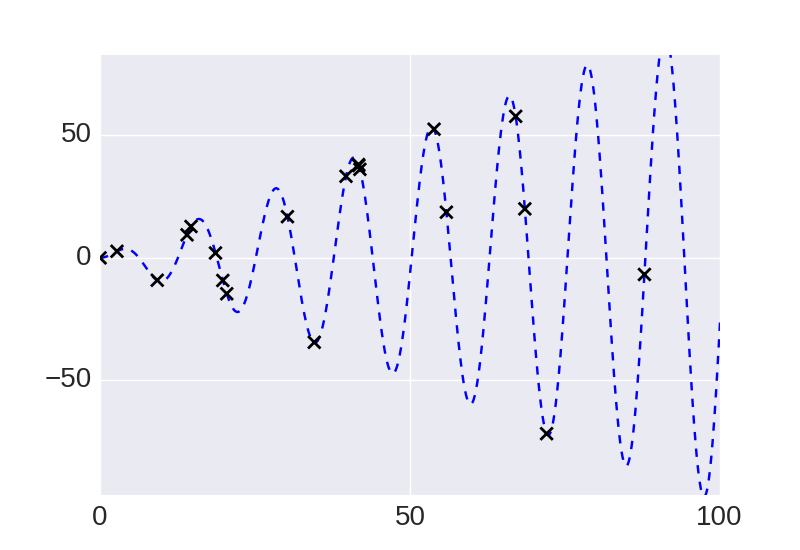
\includegraphics[width=\textwidth]{figs/composition/composition_demo_raw_data.png}
        \caption{Raw Data}
    \end{subfigure}
    ~ %add desired spacing between images, e. g. ~, \quad, \qquad, \hfill etc. 
      %(or a blank line to force the subfigure onto a new line)
    \begin{subfigure}[b]{0.45\textwidth}
\small
     \begin{align*}
    \text{LIN} &=   \sigma_1^2(x x^\prime)\\
    \text{PER} &=  \sigma_2^2 \exp \bigg( \frac{2 \sin^2 ( \pi (x - x^\prime)/p}{\ell^2} \bigg)\\ 
    \text{LIN} \times \text{PER} &=  \sigma_1^2(x x^\prime)\, \sigma_2^2 \exp \bigg( \frac{2 \sin^2 ( \pi (x - x^\prime)/p}{\ell^2} \bigg) 
    \end{align*}\vspace{5mm} 
        \caption{Kernels}
    \end{subfigure}\vspace{4mm} 


Parameterized Kernels:\vspace{3mm} 

     \begin{subfigure}[b]{0.3\textwidth}
      \centering \footnotesize
       $20.1^2(x x^\prime) $ \vspace{2mm}
	\caption{LIN}
    \end{subfigure}
    ~ %add desired spacing between images, e. g. ~, \quad, \qquad, \hfill etc. 
      %(or a blank line to force the subfigure onto a new line)
    \begin{subfigure}[b]{0.3\textwidth}
      \centering \footnotesize
      $19.1^2 \exp \bigg( \frac{2 \sin^2 ( \pi (x - x^\prime)/37.7}{6.3^2} \bigg)$ 
	\caption{PER}
    \end{subfigure}
    ~ %add desired spacing between images, e. g. ~, \quad, \qquad, \hfill etc. 
    %(or a blank line to force the subfigure onto a new line)
    \begin{subfigure}[b]{0.3\textwidth}
    \centering \footnotesize
      $383.9^2 (x x^\prime) \exp \bigg( \frac{2 \sin^2 ( \pi (x - x^\prime)/37.7}{6.3^2} \bigg)$ 
        \caption{LIN $\times$ PER}
    \end{subfigure} \vspace{4mm} 

Prior:

     \begin{subfigure}[b]{0.3\textwidth}
        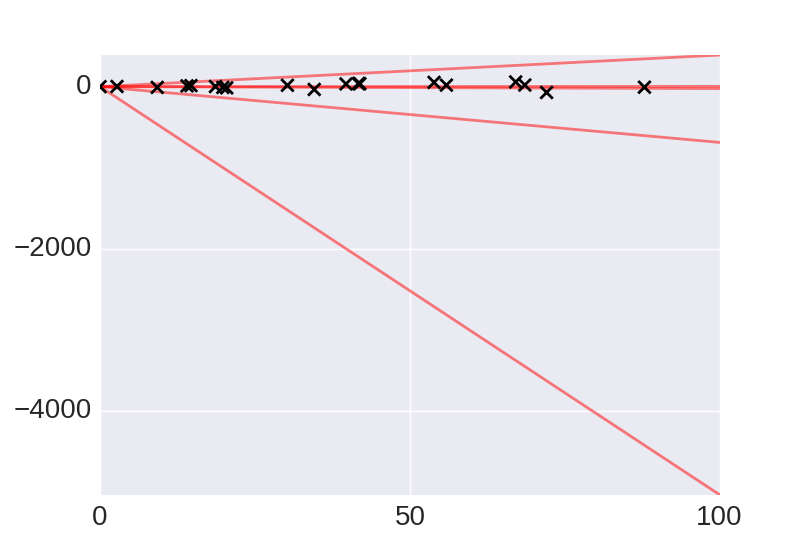
\includegraphics[width=\textwidth]{figs/composition/composition_demo_LIN_prior.png}
        \caption{LIN}
    \end{subfigure}
    ~ %add desired spacing between images, e. g. ~, \quad, \qquad, \hfill etc. 
      %(or a blank line to force the subfigure onto a new line)
    \begin{subfigure}[b]{0.3\textwidth}
        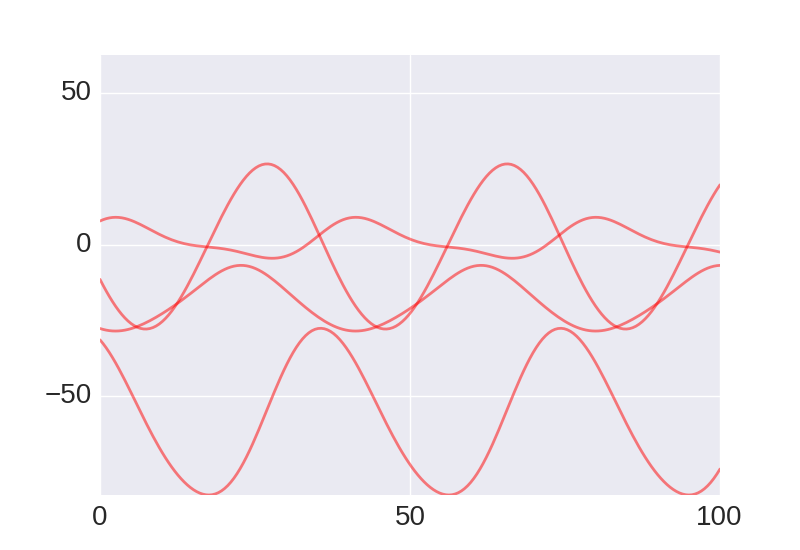
\includegraphics[width=\textwidth]{figs/composition/composition_demo_PER_prior.png}
        \caption{PER}
    \end{subfigure}
    ~ %add desired spacing between images, e. g. ~, \quad, \qquad, \hfill etc. 
    %(or a blank line to force the subfigure onto a new line)
    \begin{subfigure}[b]{0.3\textwidth}
        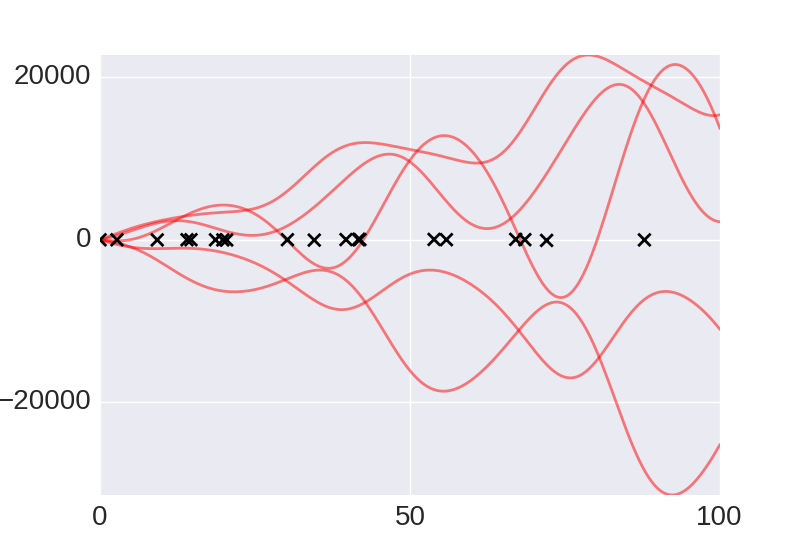
\includegraphics[width=\textwidth]{figs/composition/composition_demo_LINxPER_prior.png}
        \caption{LIN $\times$ PER}
    \end{subfigure} \vspace{4mm} 

Posterior:

 \begin{subfigure}[b]{0.3\textwidth}
        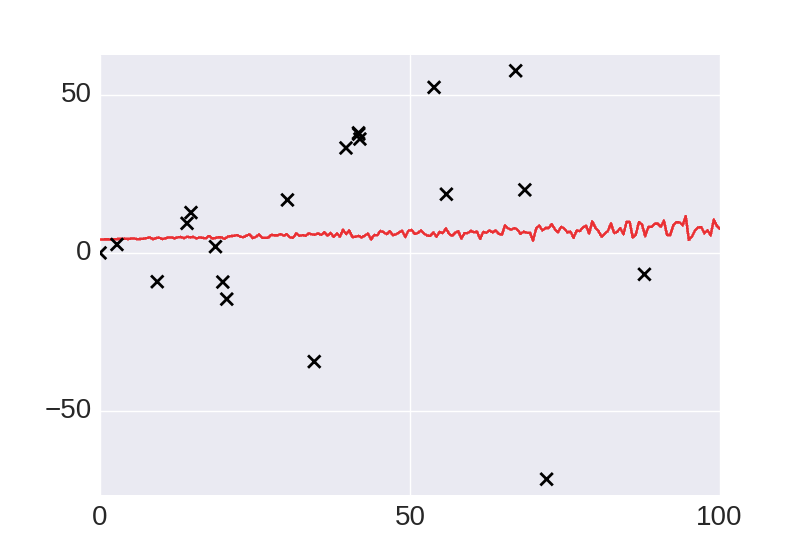
\includegraphics[width=\textwidth]{figs/composition/composition_demo_LIN.png}
        \caption{LIN}
    \end{subfigure}
    ~ %add desired spacing between images, e. g. ~, \quad, \qquad, \hfill etc. 
      %(or a blank line to force the subfigure onto a new line)
    \begin{subfigure}[b]{0.3\textwidth}
        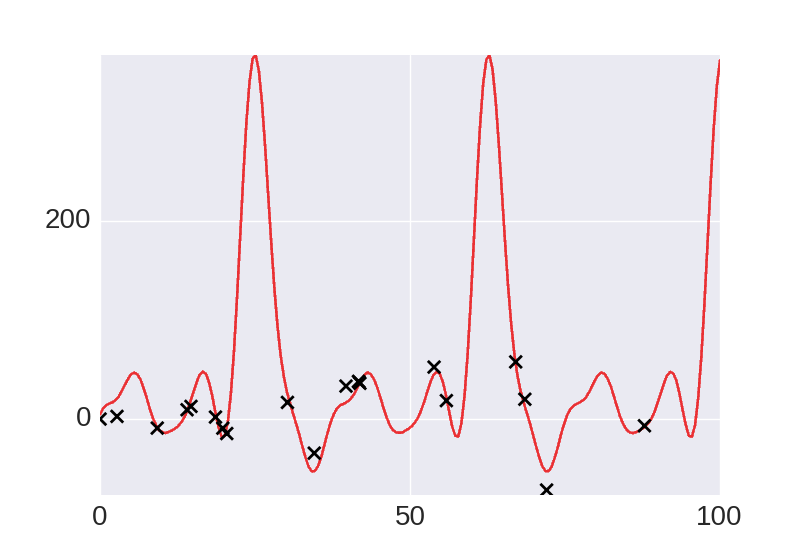
\includegraphics[width=\textwidth]{figs/composition/composition_demo_PER.png}
        \caption{PER}
    \end{subfigure}
    ~ %add desired spacing between images, e. g. ~, \quad, \qquad, \hfill etc. 
    %(or a blank line to force the subfigure onto a new line)
    \begin{subfigure}[b]{0.3\textwidth}
        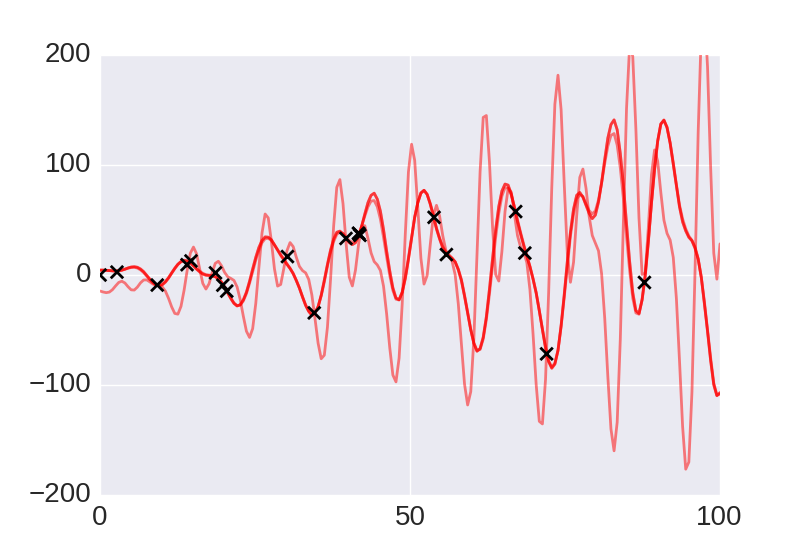
\includegraphics[width=\textwidth]{figs/composition/composition_demo_LINxPER.png}
        \caption{LIN $\times$ PER}
    \end{subfigure}

%20.0739791735
%6.31647597198
%37.7184218042
%19.1051376016

\caption{We depict kernel composition. 
(a) shows raw data (black) generated with a sine function with linearly growing amplitude (blue).
This data is used for all the plots (c-h). 
(b) shows the linear and the periodic base kernel as well as a composition of both. 
The multiplication of the two kernels indicates local interaction. The local interaction we account for in this case is the growing amplitude (a). For each column (c-h) $\bm{\theta}$ is different.(c-e) show samples from the prior
prior predictive $\fbf_*$ where random parameters are used, that is, we sample before any data points are observed.
(f-h) show samples from the predictive posterior $\hat\fbf$, after the data has been observed.}
\label{fig:composition_tutorial}
\end{figure}
%%%%%%%%%%%%%%%%%%%%%%%%%%%%%%%%%%%%%%%%%%%%%%%%%%%%%%%%%%%%
These high-level properties are compositional via addition and multiplication of different covariance functions. 
That means that we can also combine these properties.
By using multiplication of kernels we can model a local interaction of two components, for example 
%%%%%%%%%%%%%%%%%%%%%%%%%%%%%%%%%%%%%%%%%%%%%%%%%%%%%%%%%%%%
\begin{equation}\label{eq:LINxPER}
    \text{LIN} \times \text{PER} =  \sigma_1^2(x x^\prime)\, \sigma_2^2 \exp \bigg( \frac{2 \sin^2 ( \pi (x - x^\prime)/p}{\ell^2} \bigg) 
\end{equation}
%%%%%%%%%%%%%%%%%%%%%%%%%%%%%%%%%%%%%%%%%%%%%%%%%%%%%%%%%%%%
This results in a combination of the higher level properties of linearity and  periodicity.
In Fig \ref{fig:composition_tutorial} (e) we depict samples for $\fbf_*$ that are periodic
with linearly increasing amplitude.
We consider this a local interaction because the actual interaction depends on the similarity
of two data points.
An addition of covariance functions models a global interaction, that is an interaction of two high-level components that is qualitatively not dependent on the input space. An example for this a periodic function with a linear
trend.

Covariance functions come with  free parameters that we call hyper-parameters which we will
refer to as $\bm{\theta}$.
For each kernel type, each $\bm{\theta}$ is different, that is, in (\ref{eq:LIN1}) we have $\thetabf=\{\sigma_1\}$,
in (\ref{eq:PER1}) we have $\bm{\theta}=\{\sigma_2,p,\ell\}$ and in 
(\ref{eq:LINxPER}) we have $\bm{\theta}=\{\sigma_1,\sigma_2,p,\ell\}$.
Adjusting these hyper-parameters changes lower level qualitative attributes such as length
scales ($\ell$) while preserving the higher level qualitative properties of the distribution
such as linearity.
We write the parameterized covariance function as $\mathbf{K}_{\bm{\theta}}(\xbf,\xbf)$ and the
covariance matrix determined by a parameterized covariance function as $\mathbf{K}_{\bm{\theta}}$.

When we observe the data, that is we condition on the input-output pairs $\{\xbf,\fbf\}$ we can sample from the 
predictive posterior $P(\hat\fbf \mid \fbf)$ given $\mathbf{K}_{\bm{\theta}}$ and respectively $\bm{\hat{\mu}}$ and $\hat{\mathbf{K}}_{\bm{\theta}}$.
If we choose suitable parameters, for example by performing inference, we can capture the underlying dynamics of the data well (see Fig. \ref{fig:composition_tutorial} (f-h)) while sampling $\hat{\fbf}$.
Note that goodness of fit is not only limited to the parameters. A too simple qualitative structure
implies unsuitable behaviour, as for example in (Fig. \ref{fig:composition_tutorial} (g)) where additional 
recurring spikes are introduced to account for the changing amplitude of the true function that 
generated the data.







\section{Venture GPs}

The Venture procedure \texttt{make-gp} takes as input a mean function and a covariance function, and outputs a procedure for sampling from a Gaussian process.
In effect, each call to this procedure samples from \eqref{eq:gpsampler} conditioned on the return values of all previous samples.
\texttt{make-gp} allows us to perform GP inference in Venture with only a few lines of code.
We can concisely express a wide variety of GPs: simple smoothing with fixed hyper-parameters, or a prior on hyper-parameters, or a custom covariance function.
Inference on hyper-parameters can be performed using Venture's built-in MH operator or a custom inference strategy.

Venture code to create and sample from a GP with a smoothing kernel and hyperparameters is shown in Listing \ref{alg:gpNeal}.
\begin{minipage}{\linewidth}
\small
\belowcaptionskip=-10pt
\begin{lstlisting}[frame=single,mathescape,label=alg:gpNeal,basicstyle=\selectfont\ttfamily]
// HYPER-PARAMETERS
assume sf = tag('hyper, gamma(1,1)))
assume l = tag('hyper, gamma(1,1)))

// COVARIANCE FUNCTION
assume se = make_squaredexp(sf, l)

// MAKE GAUSSIAN PROCESS
assume gp = make_gp( 0, se)

// INCORPORATE OBSERVATIONS
observe gp(array x[1],...x[n])= array(y[1],...,y[n])

// INFER HYPER-PARAMETERS
infer mh('hyper, one, 1)))

\end{lstlisting}
\end{minipage}


The first two lines declare the hyper-parameters.
We tag both of them to belong to the ``scope'' \texttt{'hyper}.
These tags are supplied to the inference program (in this case, MH) to specify on which random variables inference should be done.
In this \paperOrChapter, we use MH inference throughout.
Scopes may be further subdivided into blocks, on which block proposals can be made.
In this \paperOrChapter we do not use block proposals; MH inference is done on one variable at a time.

The ASSUME directives describe the GP model: \texttt{sf} and \texttt{l} (corresponding to $\sigma$ and $\ell$) are drawn from independent $\Gamma(1,3)$ distributions.
The squared exponential covariance function can be defined outside the Venture code in a conventional programming language (e.g. Python) and imported as a foreign SP.
In that way, the user can define custom covariance functions using his or her language and libraries of choice, without having to port existing code into Venture's modelling language.
In the above, the factory function \texttt{make-se}, which produces a squared exponential function with the supplied hyperparameters, is imported from Python (we have omitted the Python code).
In the next line \texttt{make-se} is used to produce a covariance function \texttt{SE}, whose (random) hyperparameters are \texttt{l} and \texttt{sf}.
Finally, we declare \texttt{GP} to be a Gaussian process with mean zero and covariance function \texttt{SE}.










\subsection{Gaussian process memoization: \gpmem}
{\bf TODO} write

\subsection{A Bayesian interpretation}
We illustrate and compare Bayesian and frequentist view points on GP with a simple example (Fig. \ref{fig:BayesVSFreq}). We show how in a simple model, two outliers can bias a maximum a posteriori inference. The data where generated with:
\begin{equation}
\label{eq:line1}
y = 2x + 15
\end{equation}
and outliers are generated with a parallel line:
\begin{equation}
\label{eq:line2}
\hat{y} = 2x + 40.
\end{equation}
We add some small amount of white noise. We generate eight data points with (\ref{eq:line1}) and two with (\ref{eq:line2}). Since we suspect the underlying data generating mechanism to be linear, we fit a linear kernel with a constant covariance as intercept and some white noise:
\begin{equation}
\mathbf{K} = \text{LIN} + \text{C} + \text{WN}.
\end{equation}
where we upper case matrix notation denotes the covariance matrix of the complete training data. Omitting the scaling parameter for the linear kernel, there are two hyperparameters to learn, that is the noise variance and the hyper-parameter for the constant function. Maximum a posteriori inference fits the single one best line and accounts for the outliers with a large noise scaling parameter. MH does better. It assigns a small amount of probability mass to a different scaling parameter and a larger constant. The resulting prediction (indicating with the predictive mean in figure \ref{fig:BayesVSFreq}) is closer to the true underlying function.   

\begin{figure}
        \centering
        \begin{subfigure}[b]{0.49\textwidth} \centering
              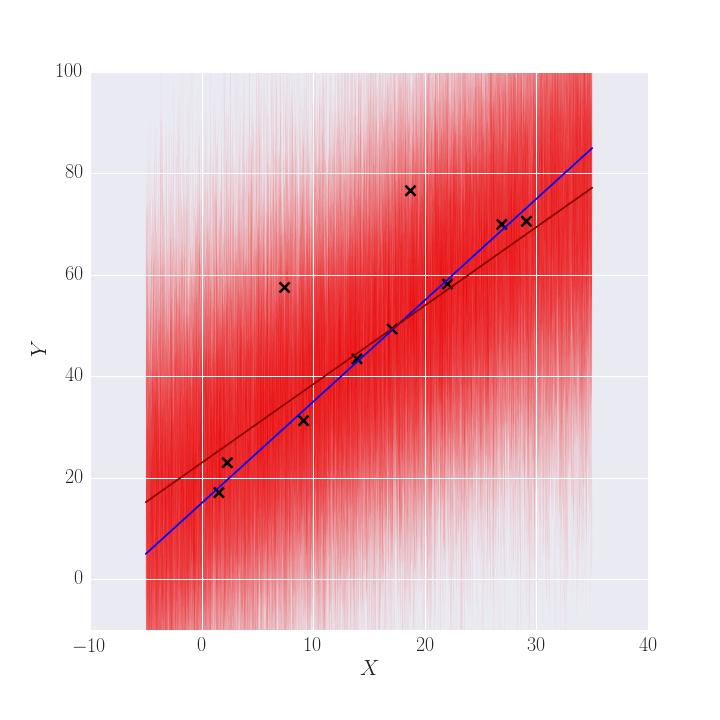
\includegraphics[height=7.5cm]{figs/MAP_linear.png}
              \caption{MAP}
                \label{fig:maplin}
        \end{subfigure}%
        \begin{subfigure}[b]{0.49\textwidth} \centering
            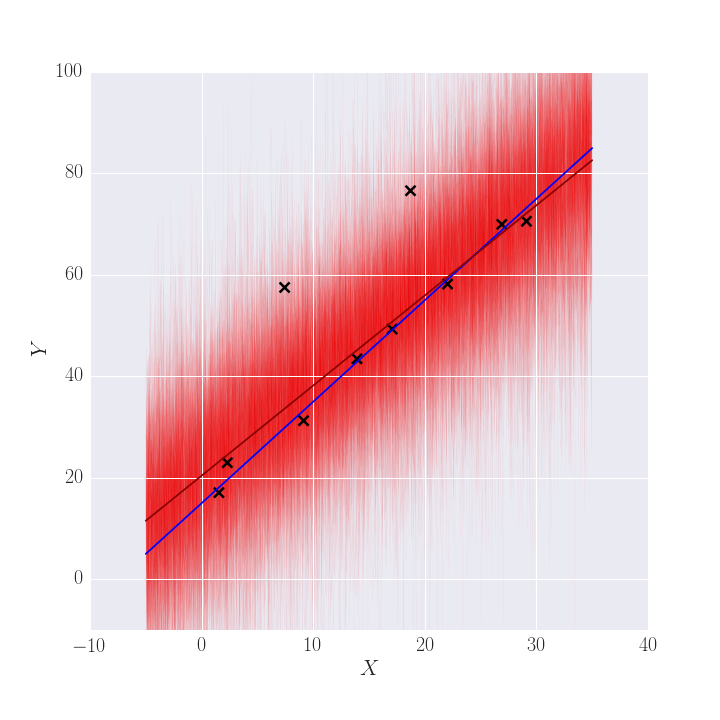
\includegraphics[height=7.5cm]{figs/MH_linear.png}
            \caption{MH}
                \label{fig:mhlin}
        \end{subfigure}%
        \caption{(a) depicts MAP inference on the data, (b) depicts MH for hyperparameter inference. The blue line is the actual data generating function. Red are samples drawn from the posterior. The dark red line is the posterior predictive mean. We see that the MH shifts the posterior closer to the ground truth than MAP.  }\label{fig:BayesVSFreq}
\end{figure}





\subsubsection{Data modelling as a special case of \gpmem}
\label{sec:special-case-gpmem}
We implement \gpmem\ by memoizing a target procedure in a wrapper that
remembers previously computed values.
This comes with interesting implications:
from the standpoint of computation, a data set of the form $\{(x_i,
y_i)\}$ can be thought of as a function $y = f_{\text{look-up}}(x)$,
where $f_{\text{look-up}}$ is restricted to only allow evaluation at a
specific set of inputs $x$.


Modelling the data set with a \ac{GP} then amounts to trying to learn
a smooth function $f_\emu$ (``emu'' stands for ``emulator'') which
extends $f$ to its full domain. We can then the incorporate
observations in two different ways: we either are either told that the
at a point \texttt{x} the value is \texttt{y}:

    \begin{lstlisting}
    observe f_emu ( x) = y
    \end{lstlisting}
Or we express this as
    \begin{lstlisting}
    predict f_compute ( x)
    \end{lstlisting}

The second expression has at least two benefits: (i) readability (in
some cases), and (ii) amenability to active learning.
As to (i), the statistical code of creating a Gaussian process is
replaced with a memoization-like idiom, which will be more familiar to
programmers.
As to (ii), when using \gpmem, it is quite easy to decide
incrementally which data point to sample next: for example, the loop
from \texttt{x[1]} to \texttt{x[n]} could be replaced by a loop in
which the next index \texttt{i} is chosen by a supplied decision rule.
In this way, we could use \gpmem\ to perform online learning using
only a subset of the available data.

We illustrate the use of \gpmem\ in this context in a tutorial in
Fig. \ref{fig:gpmem_tutorial}.

\begin{figure}
\centering
% for double arrows a la chef
% adapt line thickness and line width, if needed
\begin{tikzpicture}[thick]
\node[] (start) {};
 \node[draw,circle,minimum size=1.5cm,left = 0.5cm of start] (f) {f$_{\text{compute}}$};
 \node[draw,right = 0.5cm of start,circle,minimum size=1.5cm] (K) {$\mathbf{K}_{\theta}$};
 %\node[below left of=f_K,xshift=-1.7cm,yshift=-0.1cm] (theta) {$\bm{\theta} \sim P(\bm{\theta})$};
 \node[draw,rectangle,below=1.5cm of start, text width = 6.6cm] (gpmem) {\centering\texttt{gpmem}\vspace{2mm}
 
\small$\text{memo table} = (\mathbf{x}_{past},\mathbf{y}_{past})$\vspace{1.5mm}
 
 
\small$P(f_{emu}(x) \mid \mathbf{x}_{past},\mathbf{y}_{past})\sim \mathcal{N}(\mu(\mathbf{x}),\mathbf{K}_\theta\big(\mathbf{x},\mathbf{x})\big)$
 };
%  \node[draw,rectangle,color=ForestGreen,below = .1ex of gpmem,minimum width=1.5cm, minimum height=0.4cm,yshift=0.9cm,xshift=0.3cm] (mark) {};
  \node[draw,rectangle,dashed,right=2.2cm of K, text width = 2.2cm] (math) {\small
 $\mathbf{K}_{\theta} = \text{SE}(x,x^\prime)$\vspace{1.5mm}
 
 $\theta \;\;\,\,= \{sf,\ell \}$\vspace{1.5mm}
 
 $sf\;\, \sim P(sf)$\vspace{1.5mm}

 $\ell\;\;\;\; \sim P(\ell)$\vspace{1.5mm}
 
 
%\scriptnotesize
%
%%$\mu(\mathbf{x}) =\mu(\mathbf{x}) + \mathbf{K}_\theta(\mathbf{x},\mathbf{x}_{past})\mathbf{K}_\theta(\mathbf{x}_{past},\mathbf{x}_{past})^{-1}(\mathbf{y}_{past} - \mu(\mathbf{x}_{past}))$
 };
 \node[draw,rectangle,dashed,minimum size=1cm,left= 2.2cm of f] (resources) {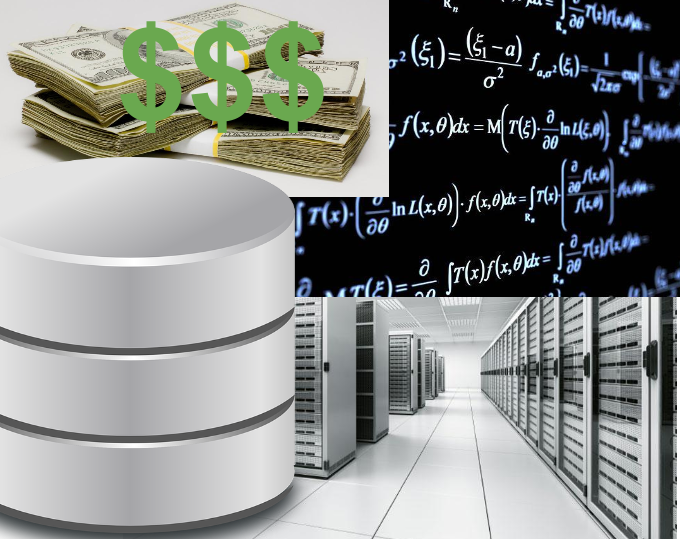
\includegraphics[width=3cm]{figs/resources.png}};

\node[draw,rectangle,below=1cm of gpmem,text width =7cm] (f_emu) {\centering $f_{emu}$ \vspace{2mm}

\begin{tabular}{l|l}\small
  $x$ & $f(x)$ \\ \hline
   $x_1$  & $y_1$ \\ 
   $x_2$  & $y_2$ \\
  $\cdots$ &   $\cdots$
 \end{tabular}
 $\;\;\;\;$
 \begin{tabular}{l}
 Parameters:\\
\small  Kernel lengthscale $\ell$  \\
\small Kernel scale-factor $sf$
 \end{tabular}

};
%\node[right = 1.2 cm of f_emu,inner sep = 0pt,outer sep=0pt,minimum size=25pt] (emu_annotate) {Infer: $\theta\;$};

\node[below = .1ex of gpmem,inner sep = 0pt,outer sep=0pt,xshift=-0.3cm] (helper1) {};
\node[below = .1ex of gpmem,inner sep = 0pt,outer sep=0pt,xshift=0.7cm] (helper2) {};

\node[above = .1ex of f_emu,inner sep = 0pt,outer sep=0pt, xshift=0mm] (helper_emu) {};

\node[above = 0.75cm of resources,inner sep = 0pt,outer sep=0pt] (helper_resource_top) {};
\node[left = 1cm of f_emu] (x_hat) {$\hat{x}$} ;
\node[right = 1cm of f_emu] (GaussianHat) {$\mathcal{N}(\hat{\bm\mu},\hat{\mathbf{K}})$} ;

%\node[right =1. cm  of f_emu, yshift=1.5cm] (infer) {\small Infer: $\ell$, $sf$} ;

% 1st pass: draw arrows

  \draw[thick,dashed,->] (resources) --node [pos=0.5,below] {resource}  node [pos=0.5,above] {outside} (f);
  \draw[thick,dashed,->] (math) -- node [pos=0.5,above] {Kernel} (K);
  \draw[thick,->] (K) -- (gpmem);
  \draw[thick,->] (f) -- (gpmem);
 % \draw[thick,->] (theta) -- (gpmem);
  \draw[thick,->] (gpmem) -- (f_emu);

 % \draw[thick,->,color=ForestGreen] (helper_compute) -- node[pos=0.5, sloped, below] {probe} (helper1);
 % \draw[thick,->,color=ForestGreen] (helper2) -- node[pos=0.5, sloped,above] {improves} (helper_emu);
   % \draw[thick,->,dashed,color=ForestGreen] (helper_resource) -- node[pos=0.5,above] {$f_{com}(x_2)=y_2$} (f_compute);
  %  \draw[thick,->,dashed,color=ForestGreen] (helper_resource) -- (resources);
     \draw[thick,->,dashed] (x_hat) -- (f_emu); 
     \draw[thick,->,dashed] (f_emu) -- (GaussianHat); 
 % \draw[thick,->] (theta) -- (gpmem);
  
   
%\path[](f_emu) edge [in=90, out=50,thick] (emu_annotate)
%    (emu_annotate) edge [->,in=310, out=270,thick]  (f_emu);
  % Note: If you have no branches, the 2nd pass is not needed

\end{tikzpicture}


\begin{tabular}{ll}
% line 1
& \\
\hline
\begin{lstlisting}[mathescape,escapechar=\#]
define f = proc( x) {
		    exp(-0.1*abs(x-2))) *
		    10* cos(0.4*x) + 0.2
		    }    
assume (f_compute f_emu) =  gpmem( f, K)
sample f_emu( array( -20, $\cdots$, 20)) 

\end{lstlisting}
& \raisebox{-0.5\height}{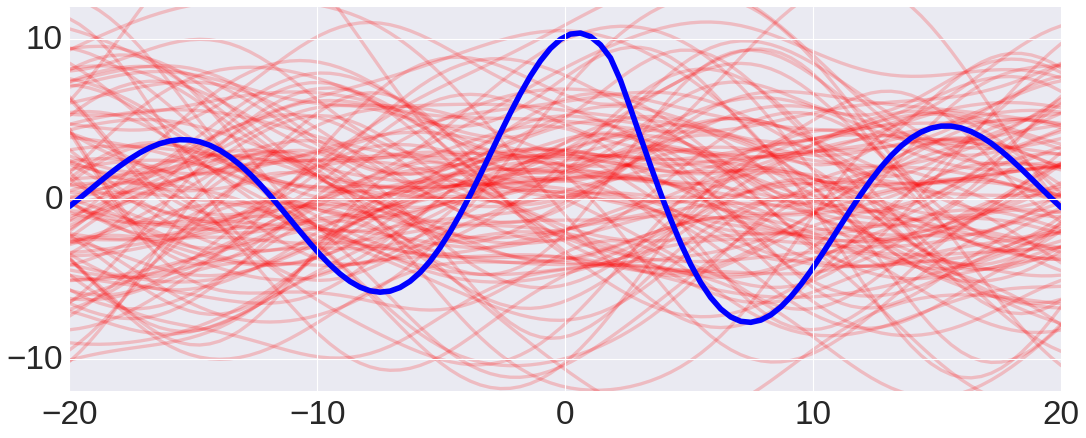
\includegraphics[height=2.5cm]{figs/tutorial_1.png}} \\ \hline
% line 2
\begin{lstlisting}[mathescape,escapechar=\#]
predict f_compute( 12.6)

sample f_emu( array( -20, $\cdots$, 20)) 

\end{lstlisting}
 &  \raisebox{-0.5\height}{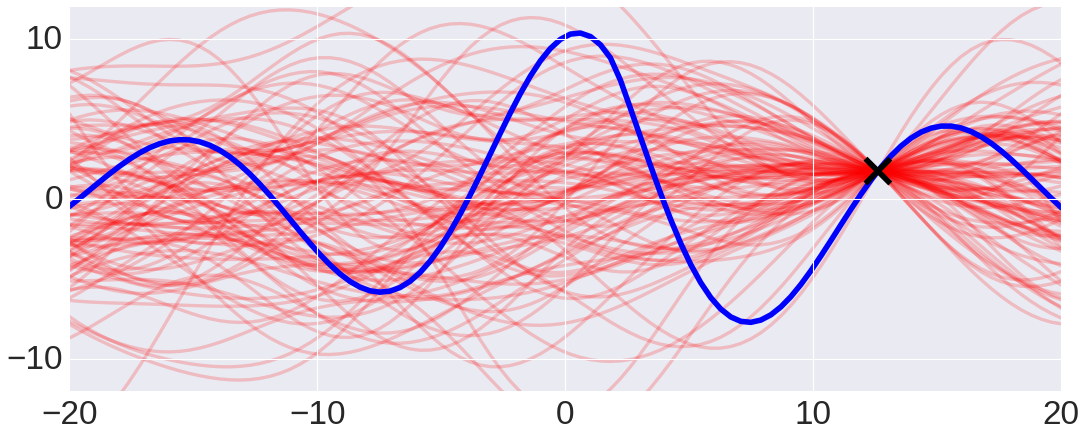
\includegraphics[height=2.5cm]{figs/tutorial_2.png}}  \\ \hline
% line 3 
 \begin{lstlisting}[mathescape,escapechar=\#]
predict f_compute( -6.4)

sample f_emu( array( -20, $\cdots$, 20)) 

\end{lstlisting}
 &  \raisebox{-0.5\height}{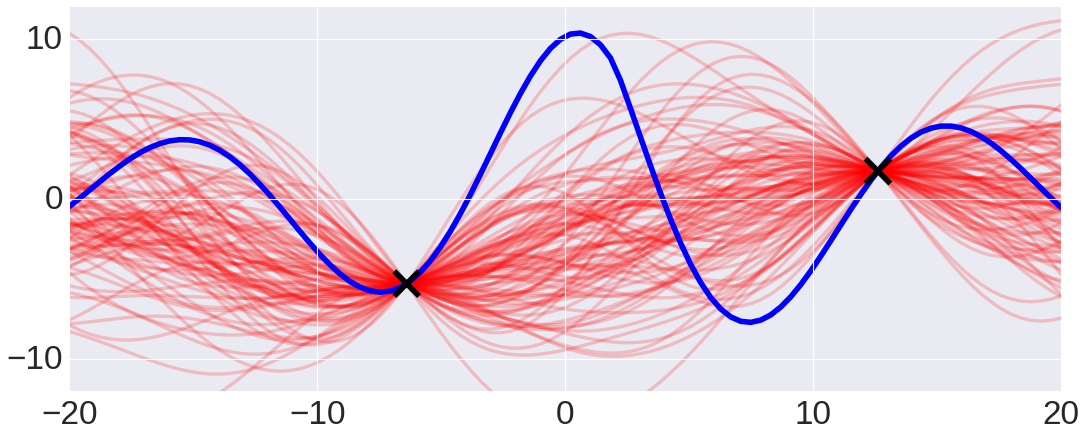
\includegraphics[height=2.5cm]{figs/tutorial_3.png}}  \\ \hline
% line 4
 \begin{lstlisting}[mathescape,escapechar=\#]
observe f_emu( -3.1) = 2.60 
observe f_emu( 7.8) = -7.60  
observe f_emu( 0.0) =  10.19

sample f_emu( array( -20, $\cdots$, 20)) 
  
\end{lstlisting}
 &   \raisebox{-0.5\height}{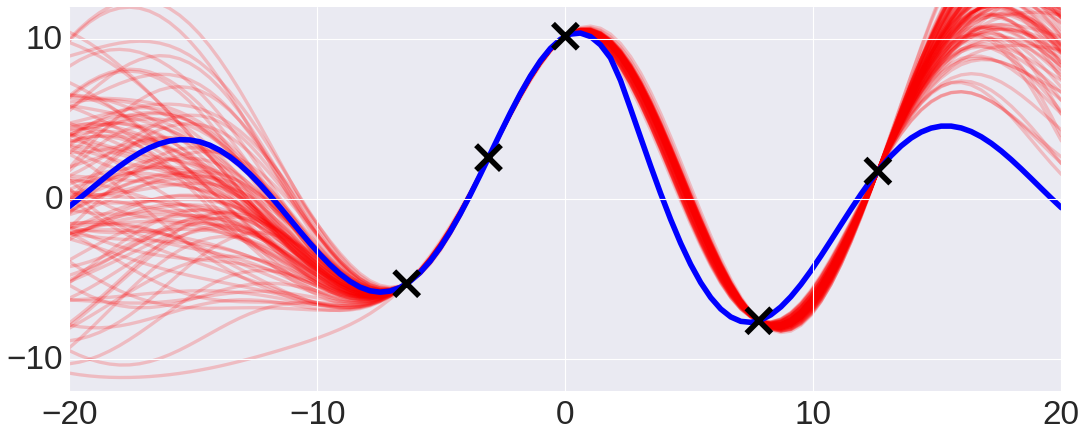
\includegraphics[height=2.5cm]{figs/tutorial_5.png}} \\ \hline
% line 5
 \begin{lstlisting}[mathescape,escapechar=\#]
infer mh(quote(hyper-parameter), one, 50)

sample f_emu( array( -20, $\cdots$, 20)) 
  
\end{lstlisting}
 &   \raisebox{-0.5\height}{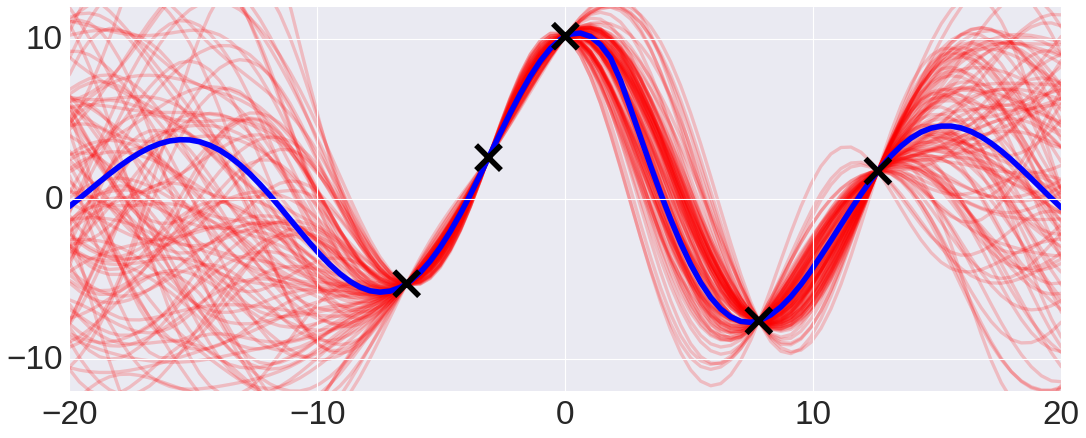
\includegraphics[height=2.5cm]{figs/tutorial_6.png}}
\end{tabular}
%\put(-245,10){\line(1,0){200}}
\put(-33,77){\color{ForestGreen}\thicklines \vector(0,-1){15}}
\put(-96,6){\color{ForestGreen}\thicklines \vector(0,-1){15}}
\put(-48,-63){\thicklines \vector(0,-1){15}}
\put(-84,-43){\thicklines \vector(0,-1){15}}
\put(-73,-68){\thicklines \vector(0,1){15}}
\caption{\gpmem\ tutorial. The top shows a schematic of \gpmem.
  \texttt{f\_compute} probes an outside resource.
  This can be expensive (top left).
  Every probe is memoized and improves the \ac{GP}-based
  emulator. Below the schematic we see a movie of the evolution
  of \gpmem's state of believe of the world given certain Venture
  directives.}
\label{fig:gpmem_tutorial}
\end{figure}

\subsubsection{The efficacy of learning hyperparameters}

The probability of the hyper-parameters of a GP with assumptions as above and given covariance function structure $\mathbf{K}$ can be described as:
\begin{equation}
\label{eq:hyperProbability}
P(\bm{\theta} \mid \mathbf{D,K}) = \frac{P(\mathbf{D} \mid \bm{\theta}, \mathbf{K})P(\bm{\theta} \mid  \mathbf{K})}{P(\mathbf{D} \mid \mathbf{K})}.
\end{equation}
Let the $\mathbf{K}$ be the sum of a smoothing and a white noise (WN) kernel. For this case, Neal suggested the problem of outliers in data as a use-case for a hierarchical Bayesian treatment of Gaussian processes~\citeyearpar{neal1997monte}\footnote{In \citep{neal1997monte} the sum of an SE plus a constant kernel is used. We stick to the WN kernel for illustrative purposes.}. The work suggests a hierarchical system of hyper-parameterization. Here, we draw hyper-parameters from a $\Gamma$ distributions:
\begin{equation}
\ell^{(t)} \sim \Gamma(\alpha_1,\beta_1),\;\sigma^{(t)} \sim \Gamma(\alpha_2,\beta_2)
\end{equation} 
and in turn sample the $\alpha$ and $\beta$ from $\Gamma$ distributions as well:
\begin{equation}
\alpha_1^{(t)} \sim \Gamma(\alpha^1_{\alpha},\beta^1_{ \alpha } ),\; \alpha_2^{(t)} \sim \Gamma(\alpha^2_{\alpha},\beta^2_{\alpha}),\cdots
\end{equation}
Assuming the covariance structure is an additive comprised of a smoothing and a white noise kernel, one can represent this kind of model using \gpmem\ with only a few lines of code:
\begin{minipage}{\linewidth}
\belowcaptionskip=-10pt
\begin{lstlisting}[frame=single,mathescape,label=alg:gphierarch,basicstyle=\selectfont\ttfamily]
/// SETTING UP THE MODEL
assume alpha_sf = tag('hyperhyper, gamma(7, 1))
assume beta_sf = tag('hyperhyper, gamma(7, 1))
assume alpha_l = tag('hyperhyper, gamma(7, 1))
assume beta_l = tag('hyperhyper, gamma(7, 1))

// Parameters of the covariance function
assume sf = tag('hyper, gamma(alpha_sf, beta_sf)))
assume l = tag('hyper, gamma(alpha_l, beta_l)))
assume sigma = tag('hyper, uniform_continuous(0, 2)) 

// The covariance function
assume se = make_squaredexp(sf, l)
assume wn = make_whitenoise(sigma)
assume composite_covariance = add_funcs(se, wn)

/// PERFORMING INFERENCE
// Create a prober and emulator using gpmem
assume f_restr = get_neal_blackbox()
assume (f_compute, f_emu) = gpmem(f_restr, composite_covariance)

// Probe all data points
predict mapv(f_compute, get_neal_data_xs())

// Infer hypers and hyperhypers
infer repeat(100, do(
    mh('hyperhyper, one, 2),
    mh('hyper, one, 1)))

\end{lstlisting}
\end{minipage}

Neal provides a custom inference algorithm setting and evaluates it using the following synthetic data problem. Let $f$ be the underlying function that generates the data:
\begin{equation}
f(x) =  0.3 + 0.4 x + 0.5 \sin(2.7x) + \frac{1.1}{(1+ x^2)} + \eta \;\;\; with\;\;\eta \sim \mathcal{N}(0,\sigma)
\end{equation}
We synthetically generate outliers by setting $\sigma = 0.1$ in $95\%$ of the cases and to $\sigma = 1$ in the remaining cases. \gpmem\  can capture the true underlying function within only 100 MH steps on the hyper-parameters to get a good approximation for their posterior (see Fig. \ref{fig:neal}). Note that Neal devices an additional noise model and performs large number of Hybrid-Monte Carlo and Gibbs steps.  
\begin{figure}
        \centering

        \begin{subfigure}[b]{0.49\textwidth} \centering
                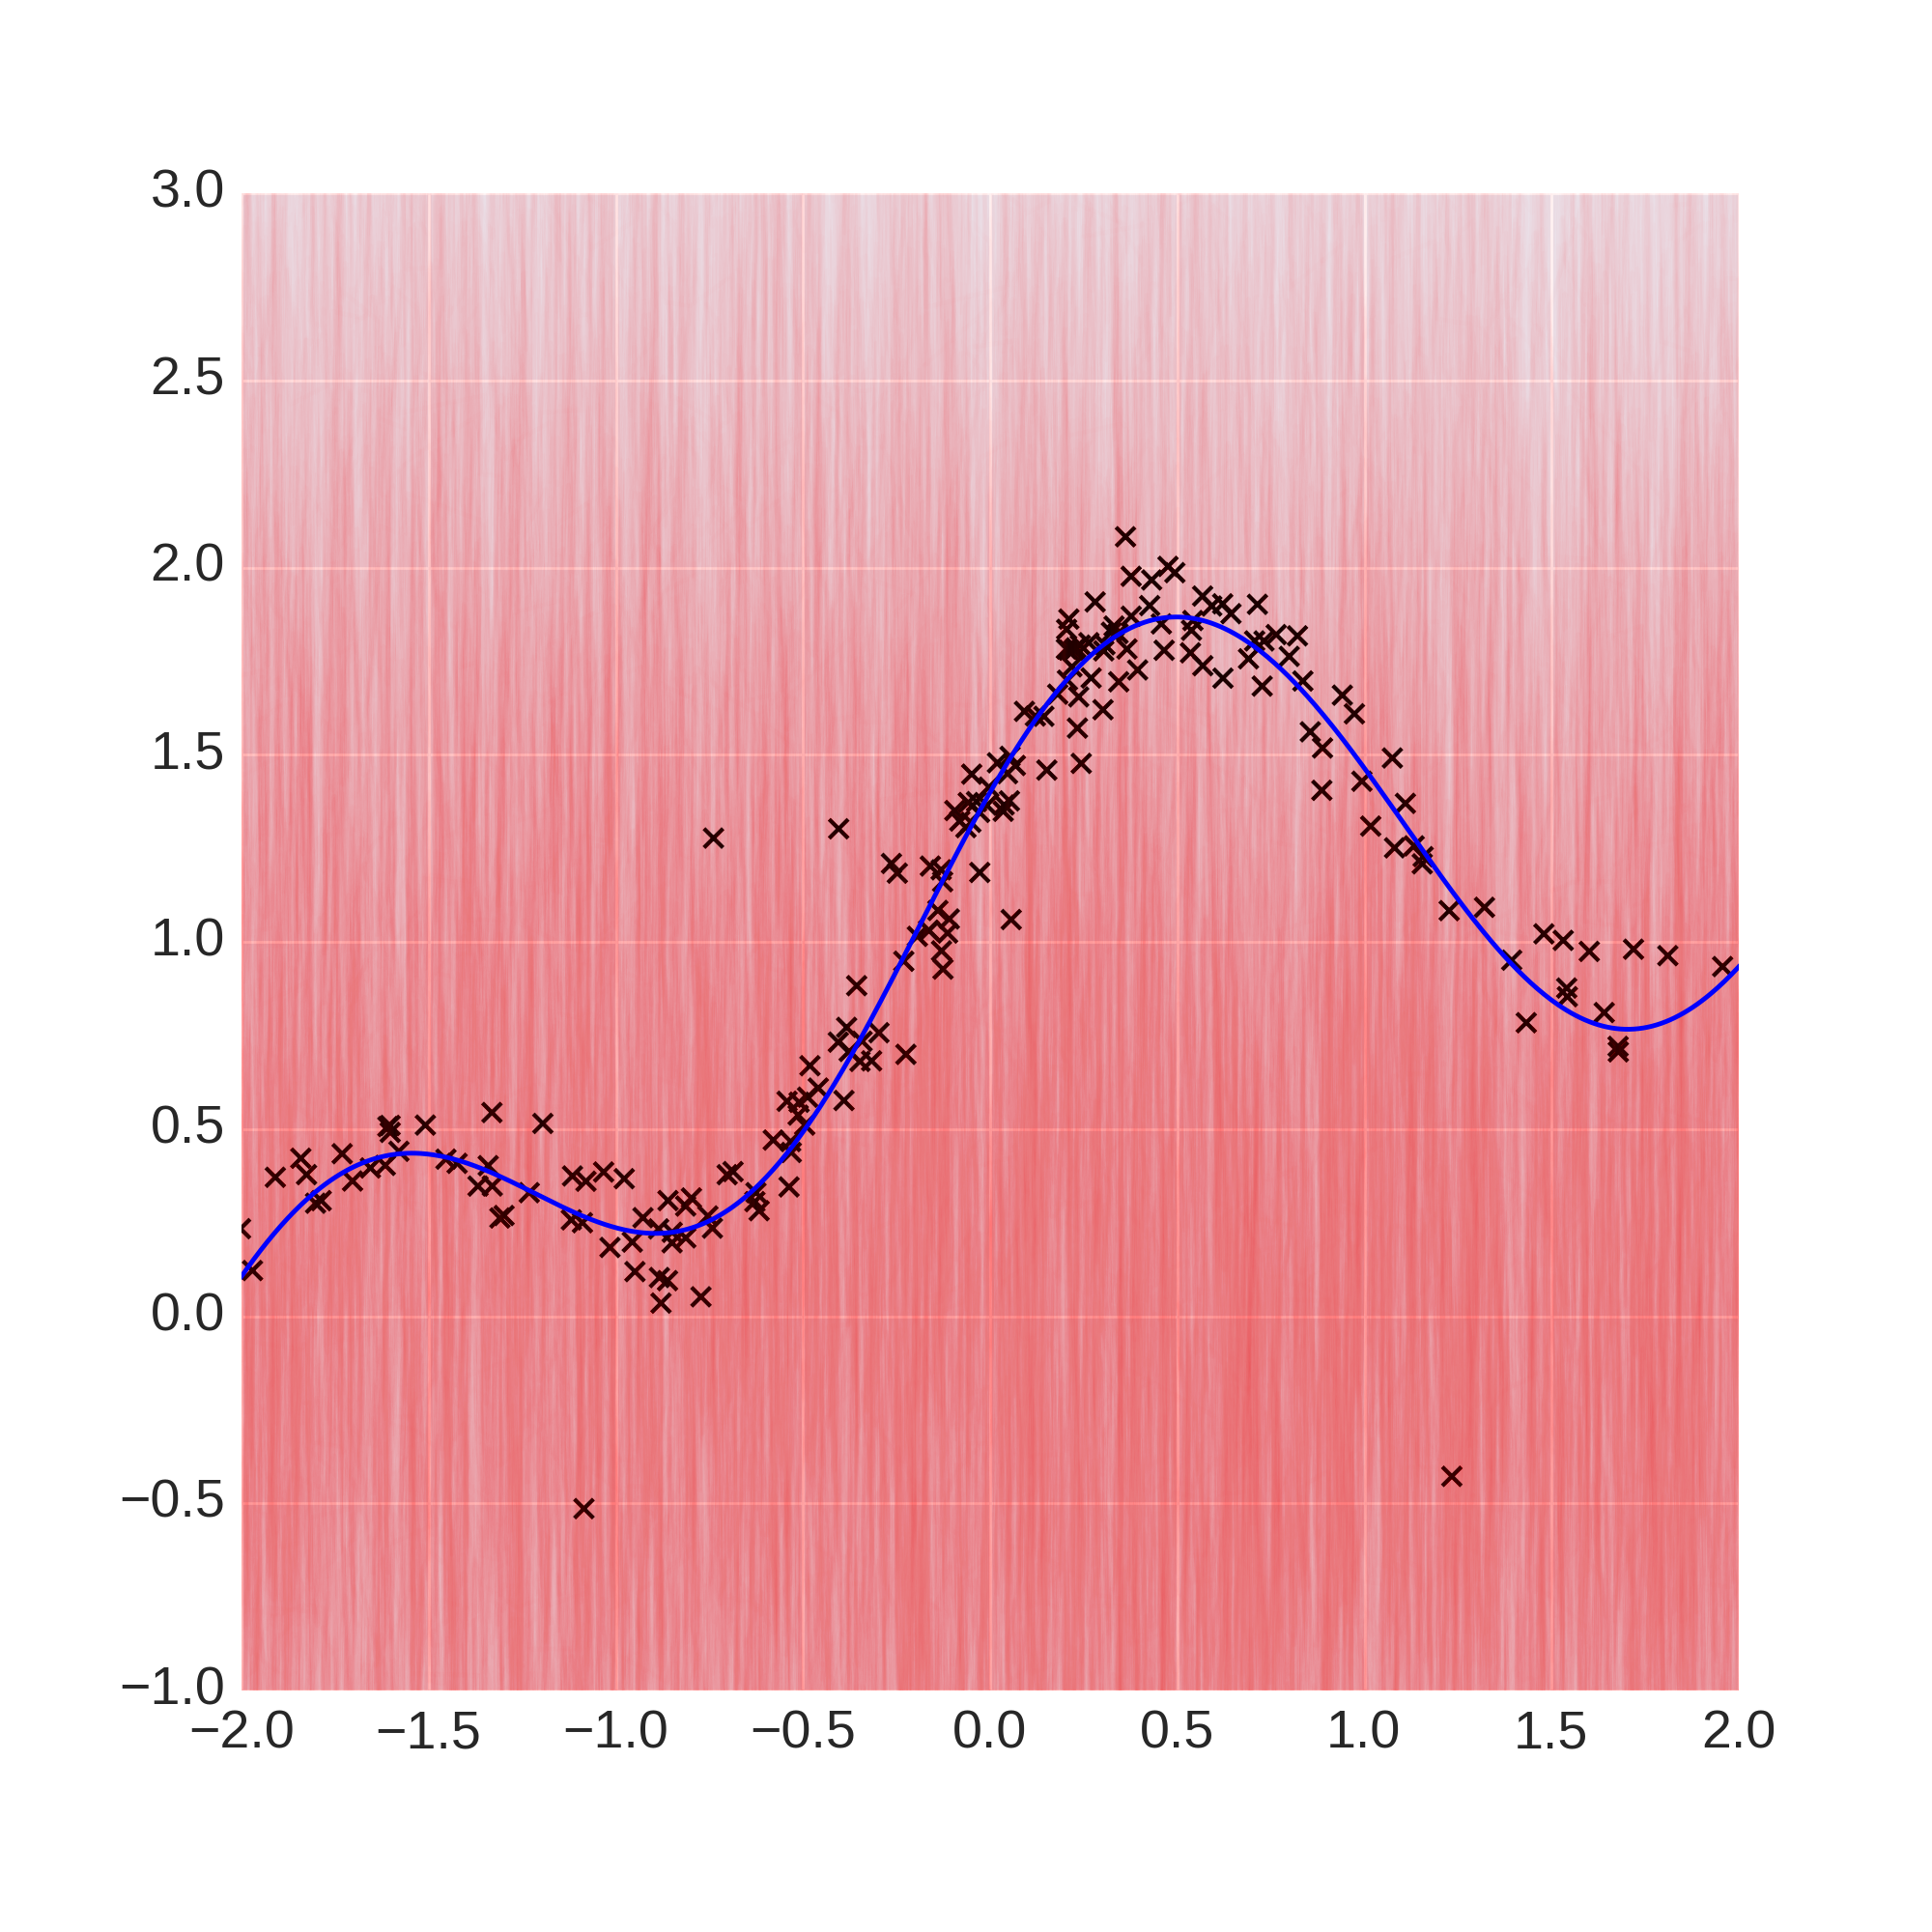
\includegraphics[height=7.5cm]{figs/neal_se_1final.png}
                \caption{Prior Inference}
                \label{fig:NealBO}
        \end{subfigure}%
        ~ %add desired spacing between images, e. g. ~, \quad, \qquad, \hfill etc.
          %(or a blank line to force the subfigure onto a new line)
        \begin{subfigure}[b]{0.49\textwidth} \centering
                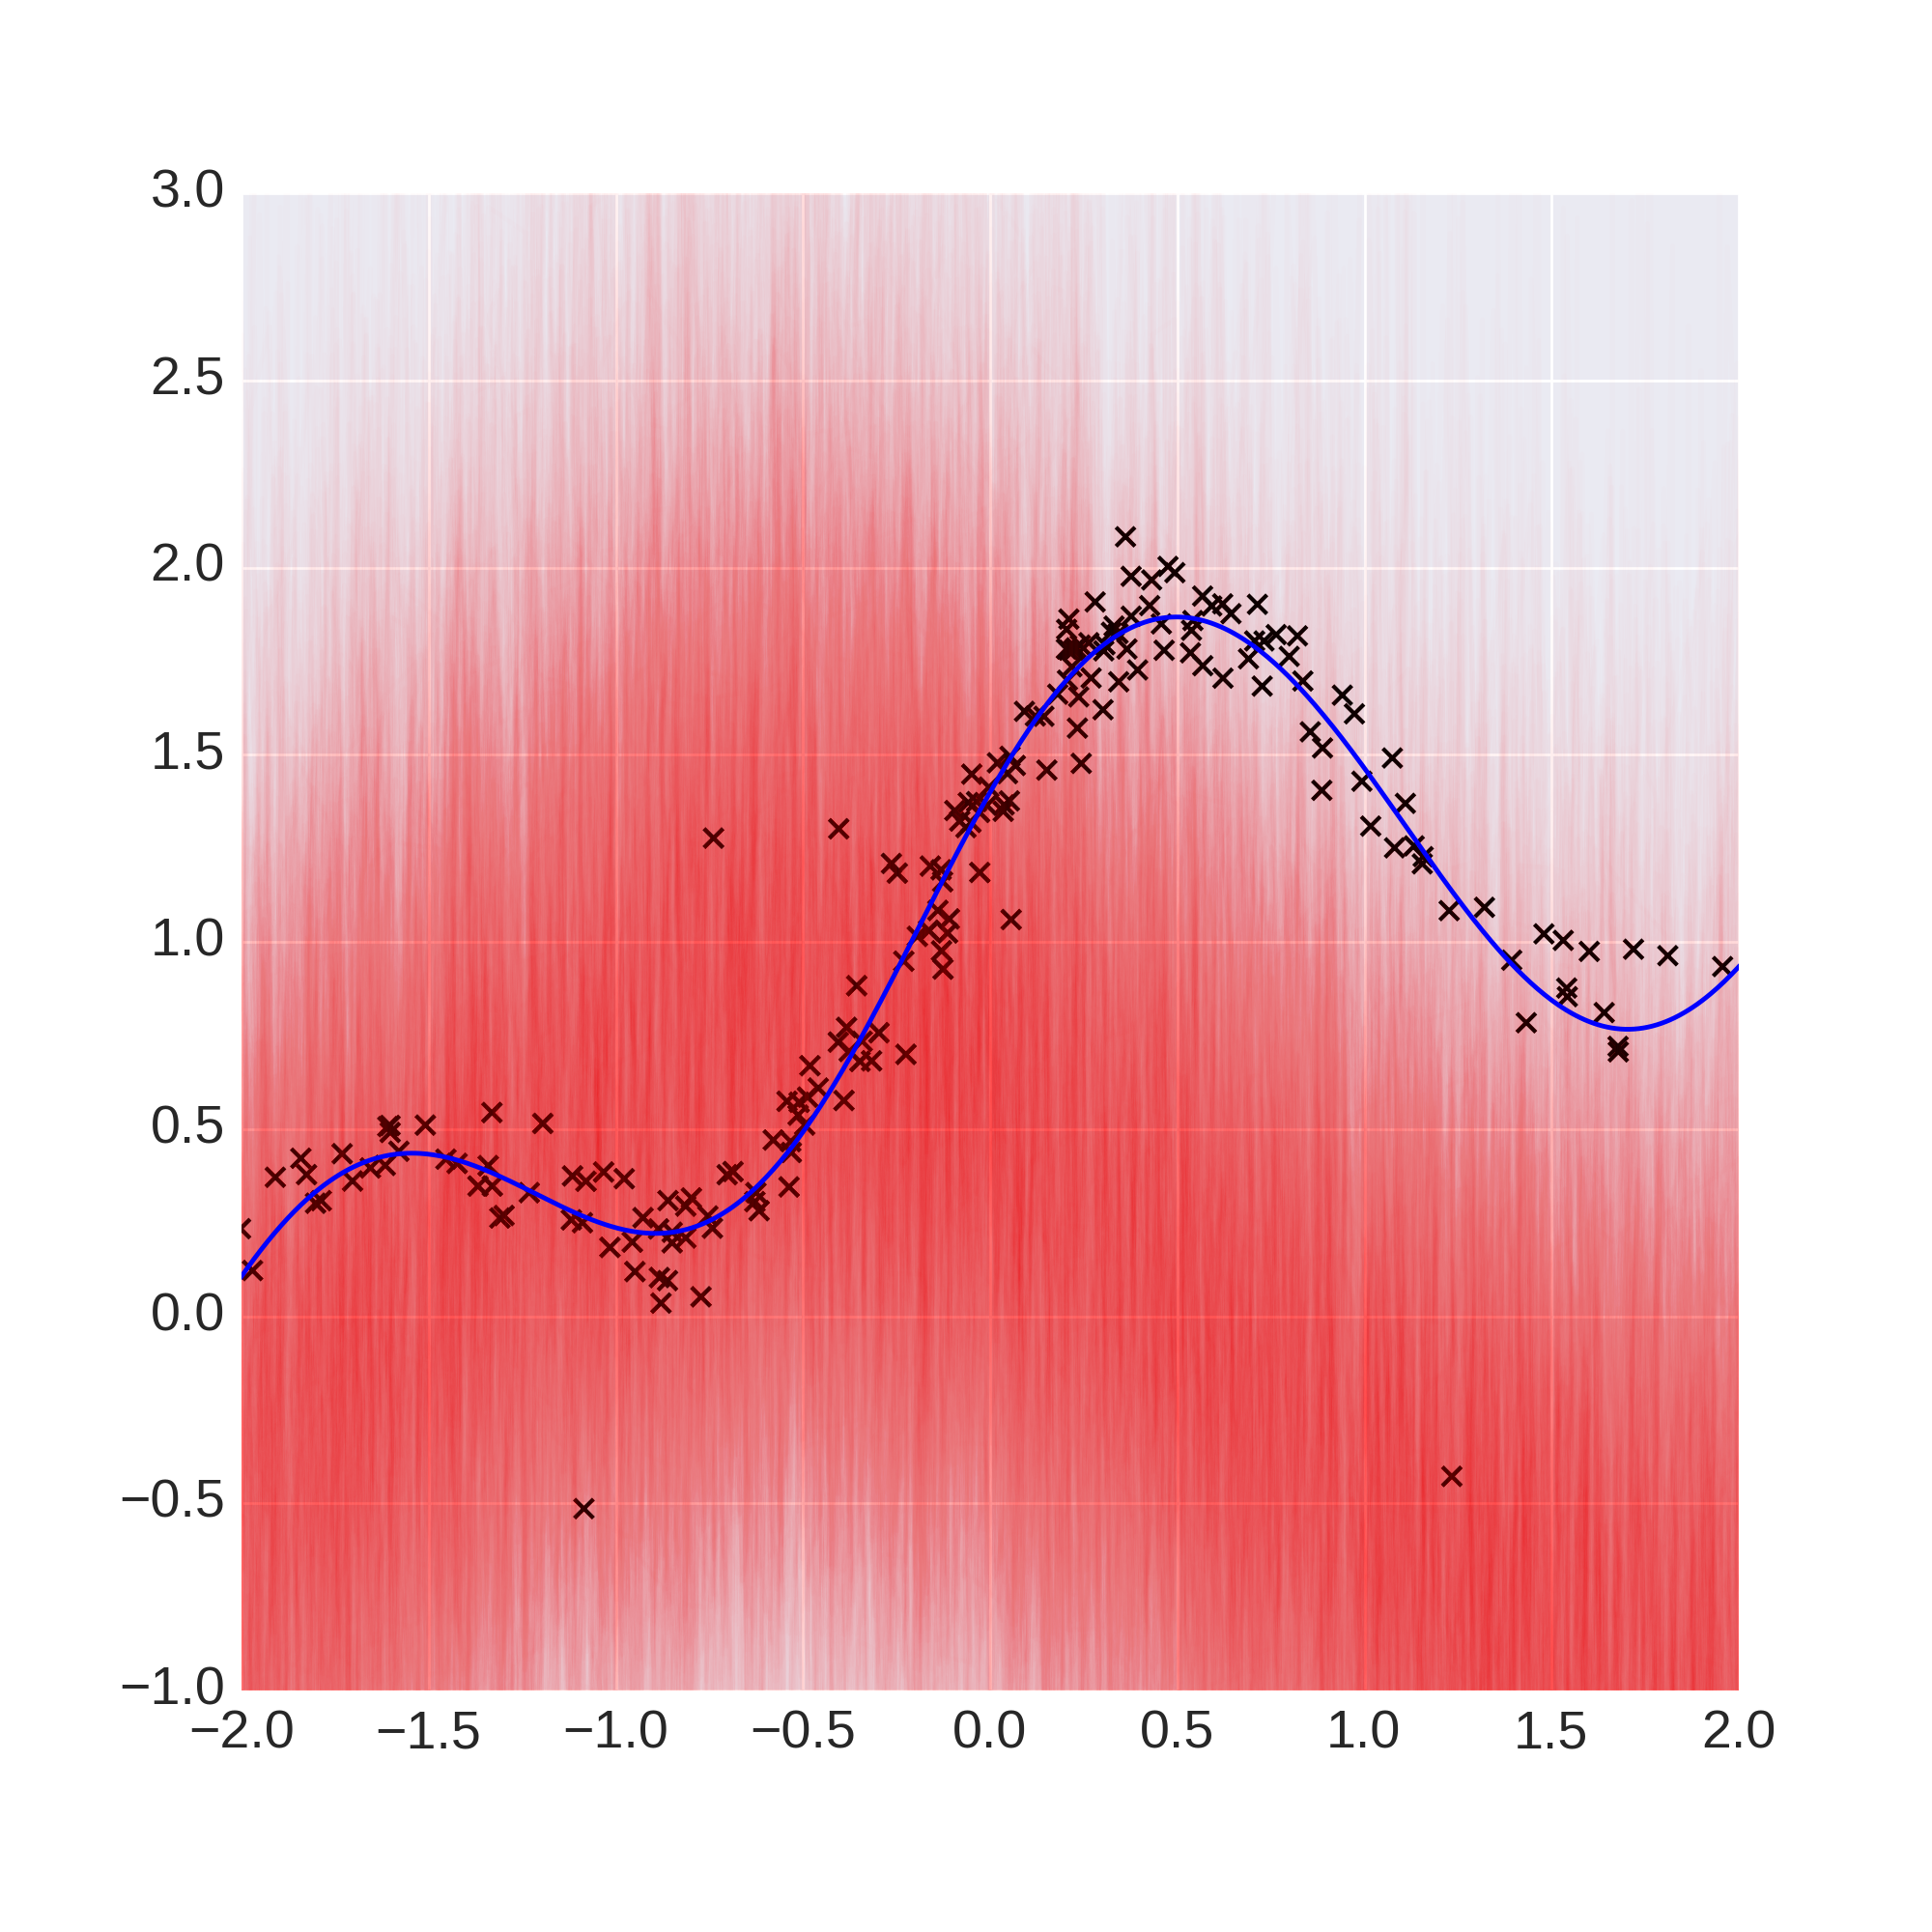
\includegraphics[height=7.5cm]{figs/neal_se_2final.png}
                \caption{Observed}
                \label{fig:NealAO}
        \end{subfigure}
        
        ~ %add desired spacing between images, e. g. ~, \quad, \qquad, \hfill etc.
          %(or a blank line to force the subfigure onto a new line)
        \begin{subfigure}[b]{0.49\textwidth} \centering
                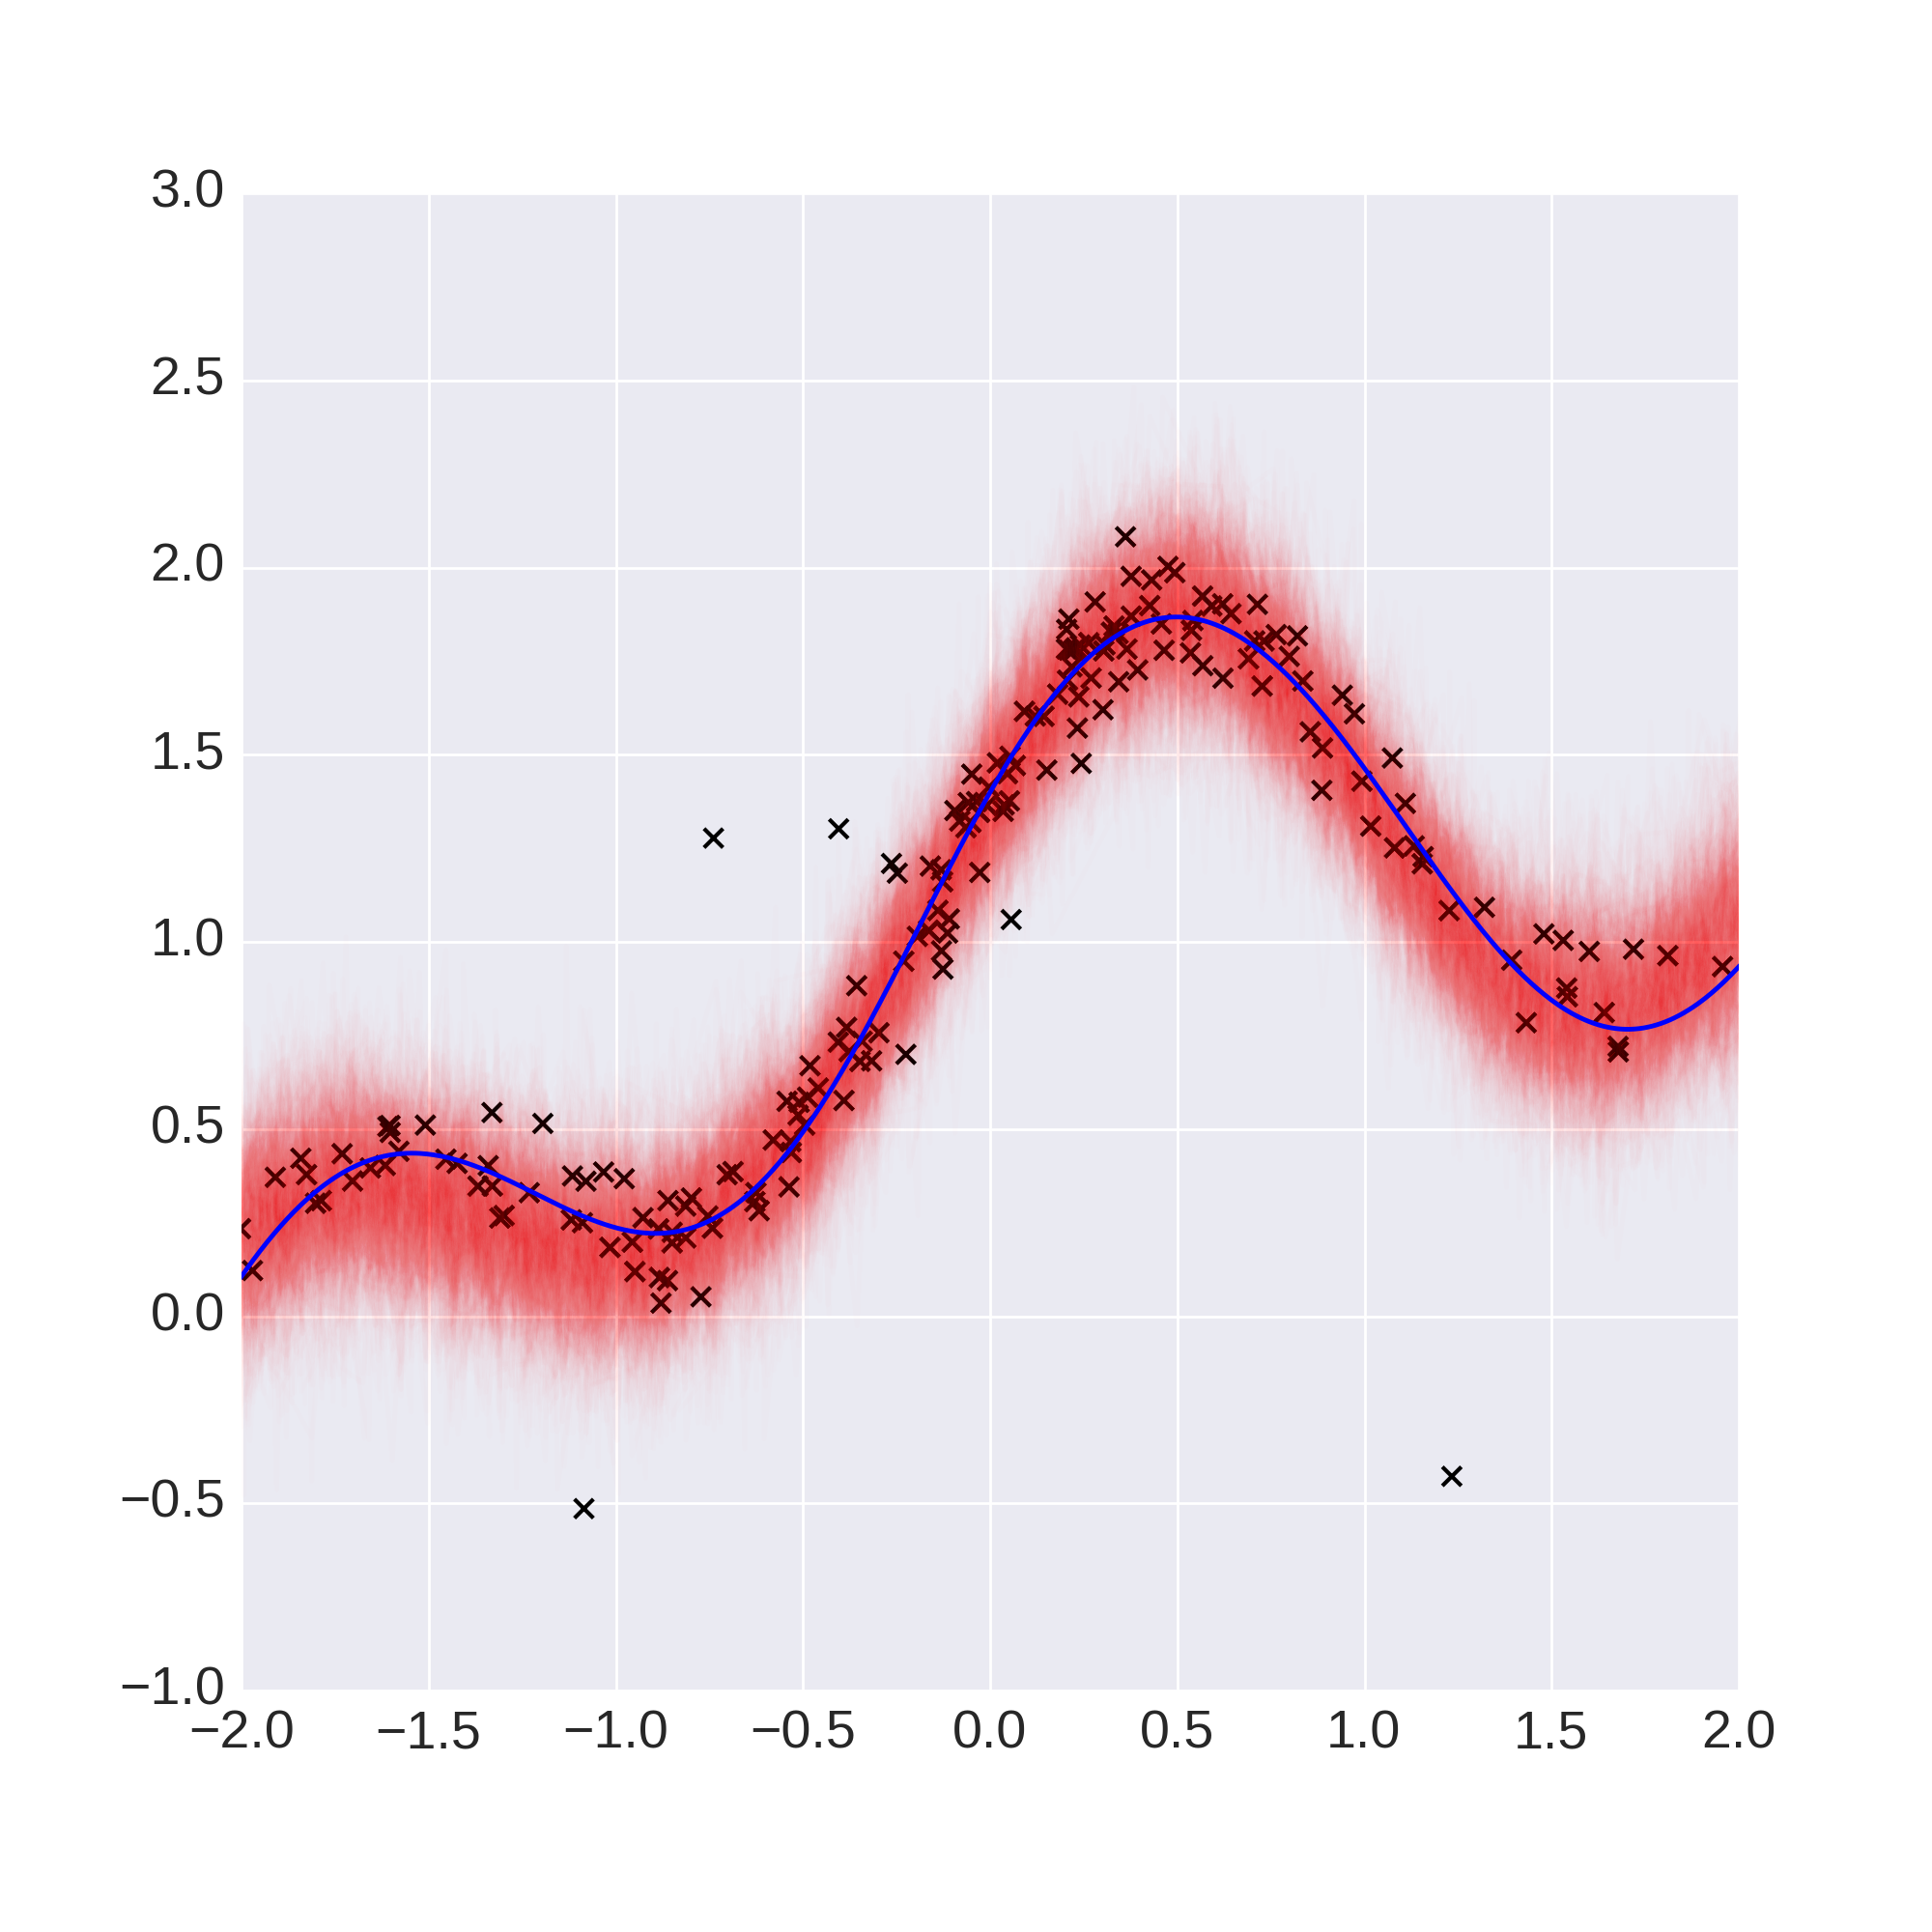
\includegraphics[height=7.5cm]{figs/neal_se_3final.png}
                \caption{Inferred}
                \label{fig:NealAI}
        \end{subfigure}
        \caption{(a)-(c) shows \gpmem\ on Neal's example. We see that prior renders functions all over the place (a). After \gpmem\ observes a some data-points an arbitrary smooth trend with a high level of noise is sampled. After running inference on the hierarchical system of hyper-parameters we see that the posterior reflects the actual curve well. Outliers are treated as such and do not confound the GP.}\label{fig:neal}
\end{figure}
We illustrate the hyper-parameter by showing the shift of the distribution on the noise parameter $\sigma$ (Fig. \ref{fig:inference}). We see that \gpmem\ learns the posterior distribution well, the posterior even exhibits a bimodal histogram when sampling $\sigma$ 100 times reflecting the two modes of data generation, that is normal noise and outliers\footnote{For this pedagogical example we have increased the probability for outliers in the data generation slightly from 0.05 to 0.2}. 

\begin{figure}
        \centering
        \begin{subfigure}[b]{0.5\textwidth} \centering
                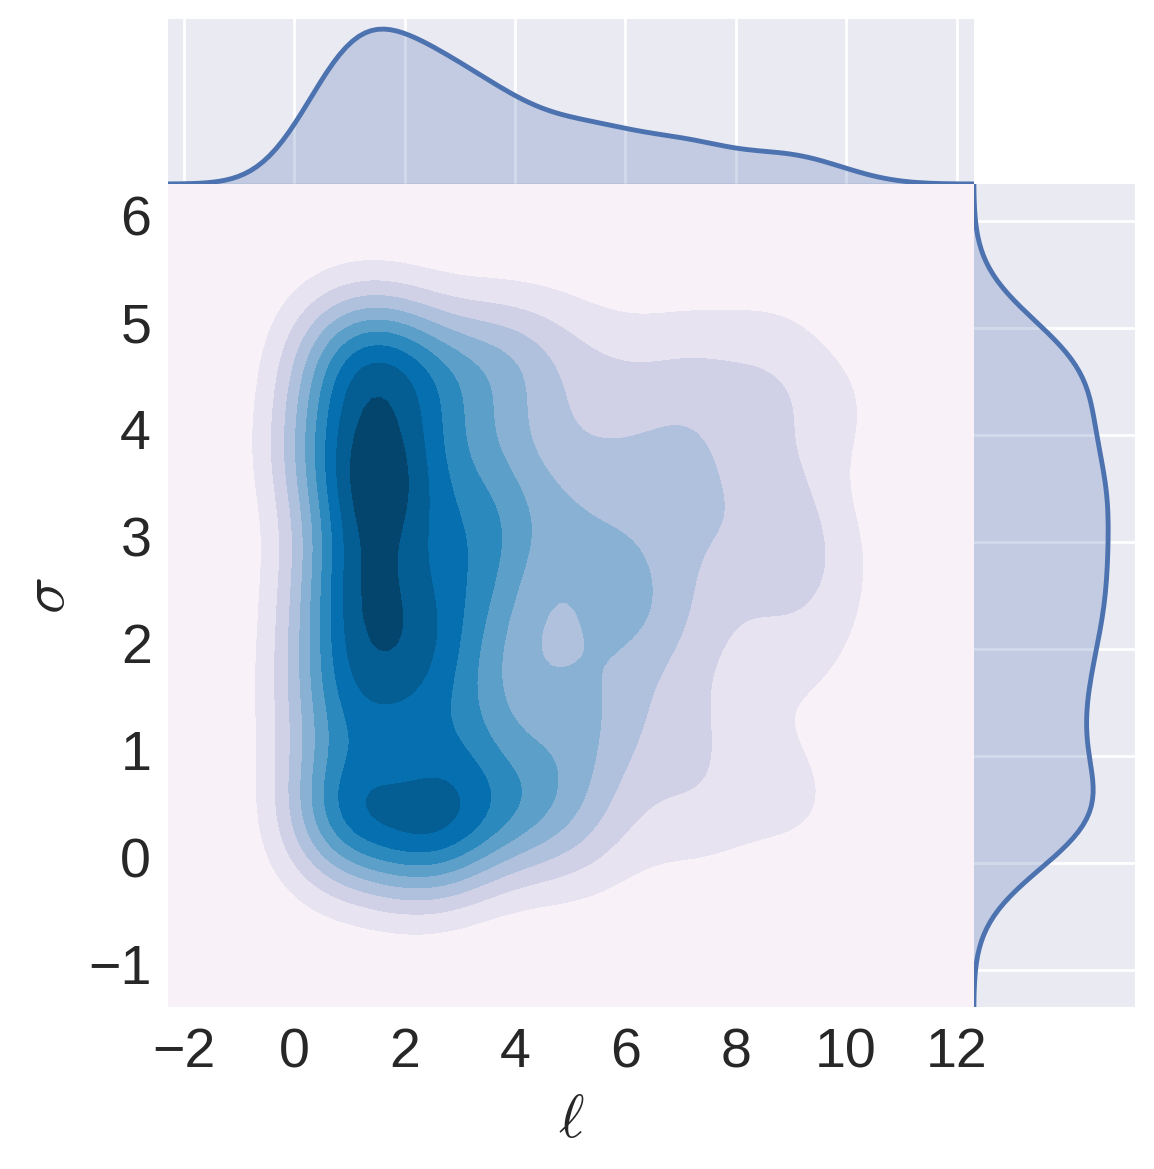
\includegraphics[height=6.5cm]{figs/neal_contour_l_vs_sigma_s__marginal_before.png}
                \caption{Before}
                \label{fig:before}
        \end{subfigure}%
        ~ %add desired spacing between images, e. g. ~, \quad, \qquad, \hfill etc.
          %(or a blank line to force the subfigure onto a new line)
        \begin{subfigure}[b]{0.5\textwidth} \centering
                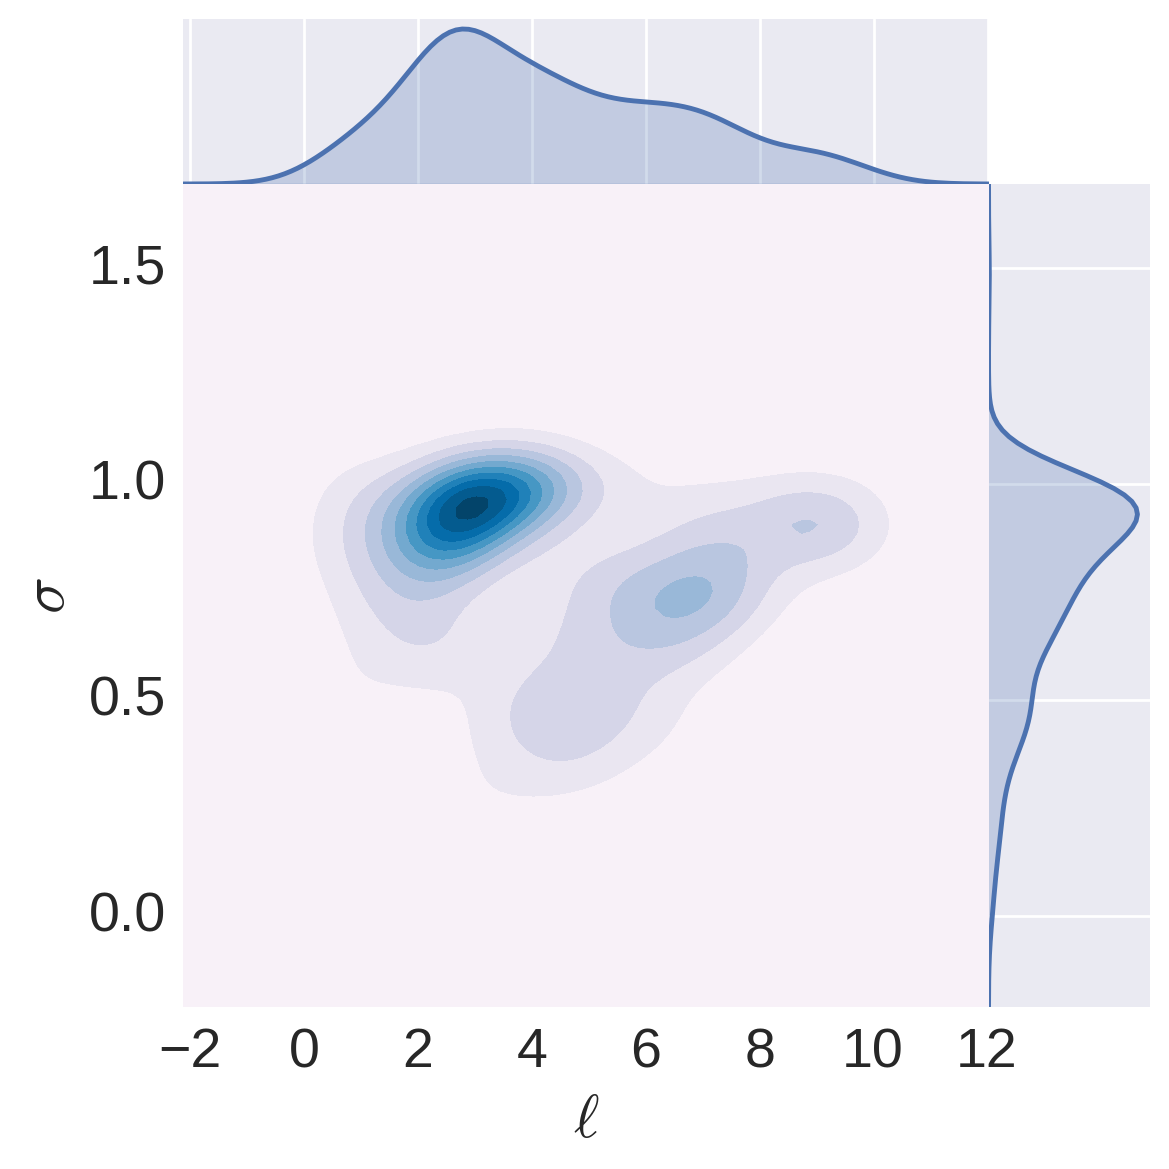
\includegraphics[height=6.5cm]{figs/neal_contour_l_vs_sigma_s__marginal_after.png}
                \caption{After}
                \label{fig:after))}
        \end{subfigure}
        \caption{Hyper-parameter inference on the parameter of the noise kernel. We show a 100 samples drawn from the distribution on $\sigma$. One can clearly recognise the shift from the uniform prior $\mathcal{U}(0,5)$ to a double peak distribution around the two modes - normal and outlier.}\label{fig:inference}
\end{figure}


\subsubsection{Broader applicability of \gpmem}\label{sec:gpmem-broader}
More generally, \gpmem\ is relevant not just when a data set is available, but also whenever we have at hand a function $f_\restr$ which is expensive or impractical to evaluate many times.
\gpmem\ allows us to model $f_\restr$ with a GP-based emulator $f_\emu$, and also to use $f_\emu$ during the learning process to choose, in an online manner, an effective set of probe points $\{x_i\}$ on which to use our few evaluations of $f_\restr$.
This idea is illustrated in detail in Section \ref{sec:bayesopt}.
Before doing this, we will illustrate another benefit of having a probabilistic programming apparatus for GP modelling: the linguistically unified treatment of inference over structure and inference over parameters.
This unification makes interleaved joint inference over structure and parameters very natural, and allows us to give a short, elegant description of what it means to ``learn the covariance function,'' both in prose and in code.
Furthermore, the example in Section \ref{sec:structurelearning} below recovers the performance of current state-of-the-art GP-based models.


\subsection{Structure Learning}\label{sec:structurelearning}
Inductive learning of symbolic expression for continuous-valued time series
data is a hard task which has recently been tackled using a greedy search over 
the approximate posterior of the possible kernel compostions for
\ac{GP}s~\citep{duvenaud2013structure,lloyd2014automatic}\footnote{\url{http://www.automaticstatistician.com/}}.

With \gpmem\ we can provide a fully Bayesian treatment of this, previously unavaible,
using a stochastic grammar  (see Fig. \ref{fig:schema}).

\begin{figure}
\centering
\usetikzlibrary{arrows, decorations.markings}
\usetikzlibrary{trees}

\tikzstyle{level 1}=[level distance=1cm, sibling distance=1.5cm]
\tikzstyle{level 2}=[level distance=1cm, sibling distance=1.1cm]

% Define styles for operators and leafs
\tikzstyle{operator} = [draw=none,circle, minimum width=1pt]
\tikzstyle{end} = [circle, minimum width=3pt,fill, inner sep=0pt]
% for double arrows a la chef
% adapt line thickness and line width, if needed

\begin{subfigure}[b]{0.49\textwidth}\centering
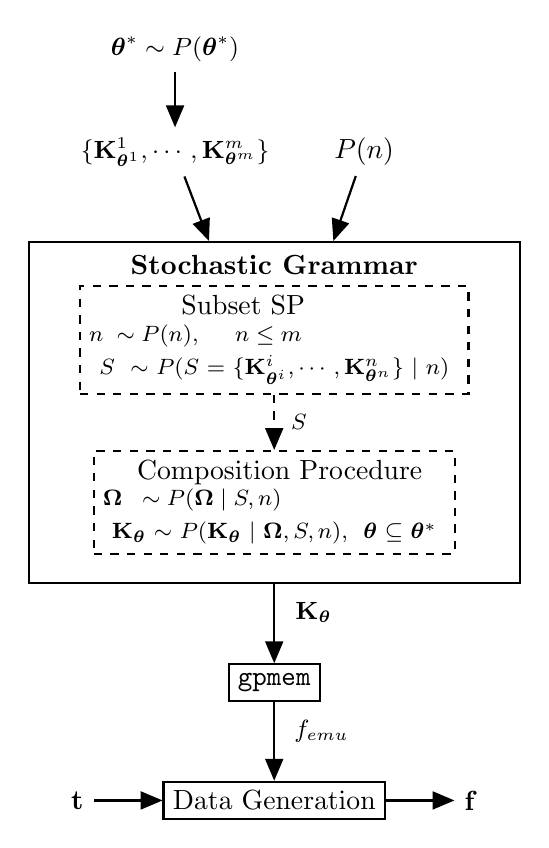
\begin{tikzpicture}[thick]
 \node[] (start) {};
 \node[left=-0.2cm of start] (base_kernels) {\small$\{\Kbf_{\bm{\theta}^1}^1,\cdots,\Kbf_{\bm{\theta}^m}^m\}$};
 \node[above=0.7cm of base_kernels] (theta) {\small$\bm{\theta}^* \sim P(\bm{\theta}^*)$};
\node[right=0.5cm of start] (n) {$P(n)$};
 \node[draw,rectangle, below=1cm of start, text width =6.0cm, text 
height=4.1cm,align=center] (grammar)
{};


 \node[draw,dashed,rectangle, below=-3.8cm of grammar, text width
=4.7cm,align=center] (subset) {
$\;\;\;\;\;\;\;\;\;\;\;\;$Subset SP % I can't believe that this is the simpliest way to
% get spacing right 
{\raggedright
\footnotesize$ n\; \sim P(n),\;\;\;\;\; n \leq m$ \\

\footnotesize$S \; \sim P(S = \{\Kbf_{\bm{\theta}^i}^i,\cdots,\Kbf_{\bm{\theta}^n}^n\} \mid n)$
}
};
 \node[draw,rectangle,dashed, below=0.7cm of subset, text width
=4.35cm,align=center]
(composition_procedure) {
$\;$Composition Procedure\\ % I can't believe that this is the simpliest way to
% get spacing right 
{\raggedright
\footnotesize$\bm{\Omega}\;\; \sim P(\bm{\Omega} \mid S,n)$ \\

\footnotesize$\Kbf_{\bm{\theta}} \sim P(\Kbf_{\bm{\theta}} \mid \bm{\Omega},S,n),\;\,\bm{\theta}\subseteq\bm{\theta}^*$
}
};

\node[above=0.0cm of subset]{\centering \bf Stochastic Grammar}; 

 \node[draw,rectangle,below=1cm of grammar] (gpmem) {\texttt{gpmem}};

 \node[draw,rectangle,below=1cm of gpmem] (f) {Data Generation};
\node[left of=f,xshift=-1.5cm] (x) {$\mathbf{t}$};
\node[right of=f,xshift=1.5cm] (y) {$\mathbf{f}$};

 \node[below=0.1cm  of grammar,xshift=0.5cm] (k)
{\small$\Kbf_{\bm{\theta}}$};


\node[below=0.1cm  of gpmem,xshift=0.6cm] (gp) {
\small$f_{emu}$};

% 1st pass: draw arrows
  \draw[thick,->] (base_kernels) -- (grammar);
  \draw[thick,->] (n) -- (grammar);
  \draw[thick,->] (theta) -- (base_kernels);
  \draw[thick,->] (grammar) -- (gpmem);
  \draw[thick,->] (gpmem) -- (f);
 \draw[thick,->] (x) -- (f);
 \draw[thick,->] (f) -- (y);
 \draw[thick,dashed,->] (subset) -- node[right]{\footnotesize $\;S$} (composition_procedure);
  % Note: If you have no branches, the 2nd pass is not needed
\end{tikzpicture}\vspace{2mm}
\caption{} 
\end{subfigure}
\begin{subfigure}[b]{0.49\textwidth}\centering
\begin{tikzpicture}[grow=right, sloped]
\node[operator] {\small $+$}
    child {
        node[operator] {\small $+$}        
            child {
               node[operator] {\small $\times$}        
        child {
                node[operator, label=right:
                    {$\cdots$}] {}
                edge from parent
                node[above] {}
                node[below]  {}
            }
            child {
                node[end, label=right:
                    {SE$_{\theta^4}$}] {}
                edge from parent
                node[above] {}
                node[below]  {}
            }
        edge from parent         
            node[above] {}
            node[below]  {}
            }
            child {
                node[end, label=right:
                    {WN$_{\theta^3}$}] {}
                edge from parent
                node[above] {}
                node[below]  {}
            }
            edge from parent 
            node[above] {}
            node[below]  {}
    }
    child {
        node[operator] {\small $\times$}        
        child {
                node[end, label=right:
                    {PER$_{\theta^2}$}] {}
                edge from parent
                node[above] {}
                node[below]  {}
            }
            child {
                node[end, label=right:
                    {LIN$_{\theta^1}$}] {}
                edge from parent
                node[above] {}
                node[below]  {}
            }
        edge from parent         
            node[above] {}
            node[below]  {}
    };
\node[xshift=-0.7cm] (K) {$\mathbf{K}_{\bm{\theta}}=$}; 
 \node[xshift=2.6cm,below =2.4cm of K] (Keq) {$\mathbf{K}_{\bm{\theta}}=\text{LIN}_{\theta^1} \times \text{PER}_{\theta^2}+\text{WN}_{\theta^3} + \text{SE}_{\theta^4} \times ( \cdots )$};
\end{tikzpicture}
\caption{} 
\end{subfigure}

\begin{subfigure}[b]{0.99\textwidth}\centering
\begin{tabular}{cccc}
\multicolumn{4}{c}{\bf Base Components} \rule{0pt}{3ex} \\ 
\small LIN: Linearity &\small PER: Periodicity &\small SE: Smoothness &\small WN: White Noise \rule{0pt}{2ex} \\
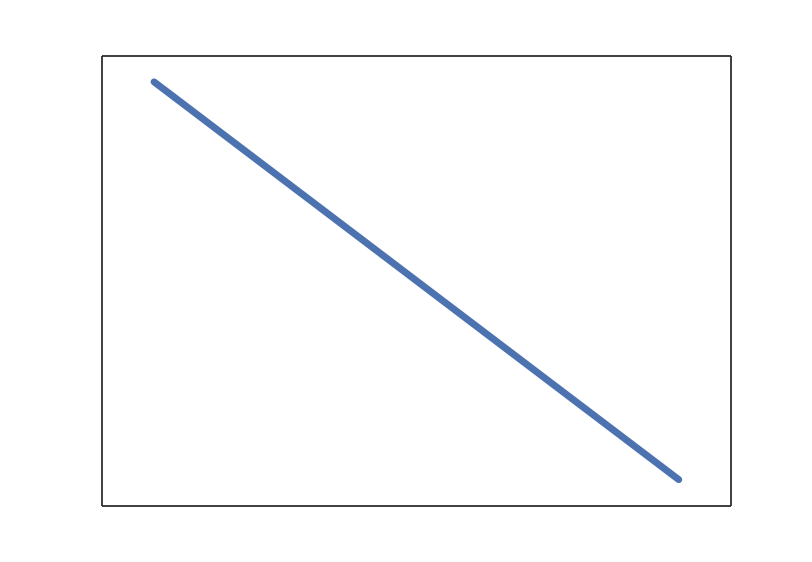
\includegraphics[height=2cm]{figs/kernel/kernelLIN.png} & 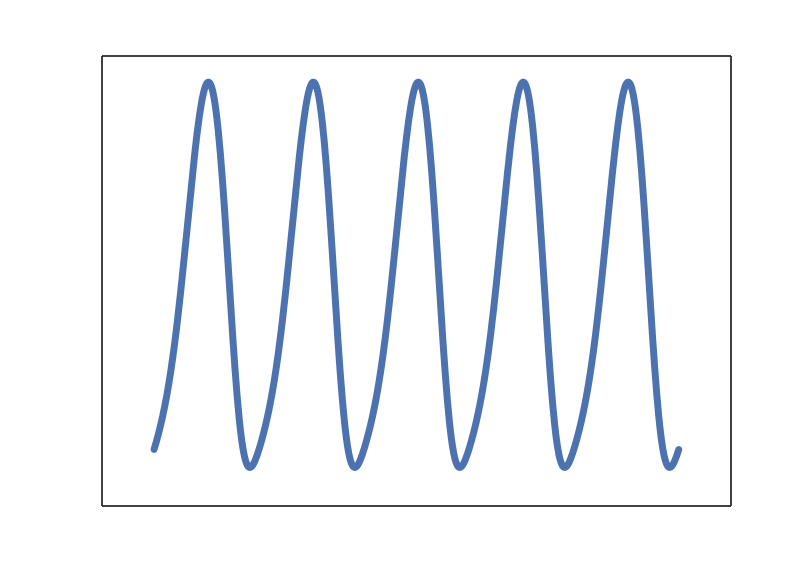
\includegraphics[height=2cm]{figs/kernel/kernelPER.png} & 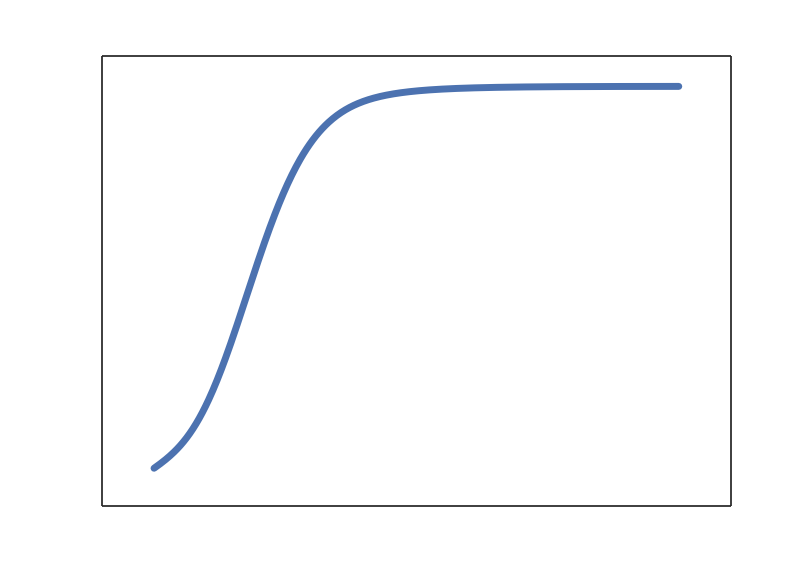
\includegraphics[height=2cm]{figs/kernel/kernelSE.png} & 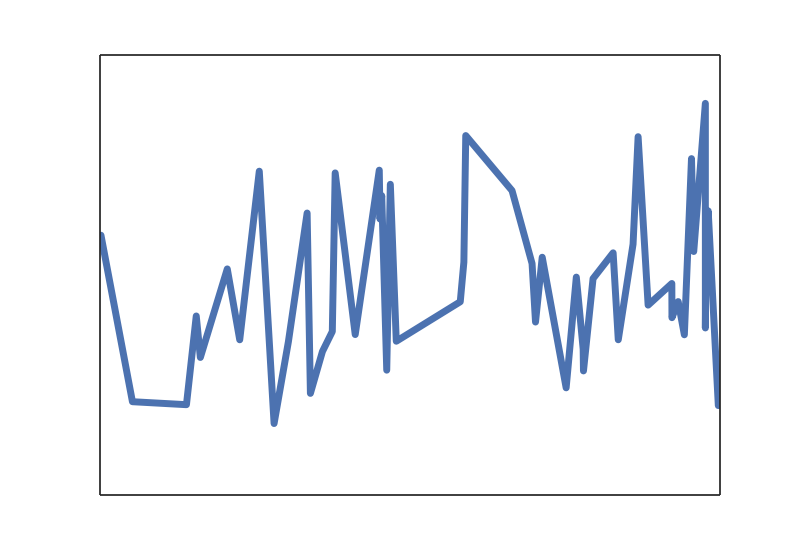
\includegraphics[height=2cm]{figs/kernel/kernelWN.png}\\
\end{tabular}
\begin{tabular}{cccc}
\multicolumn{4}{c}{\bf Composite Structure} \rule{0pt}{0ex}  \\ 
\small LIN + PER: &\small LIN $\times$ PER: &\small SE $\times$ PER: &\small LIN $\times$ LIN: \rule{0pt}{2ex} \\
\small Periodicity with Trend &\small Growing Amplitude &\small Local Periodicity&\small Quadratic \rule{0pt}{2ex} \\
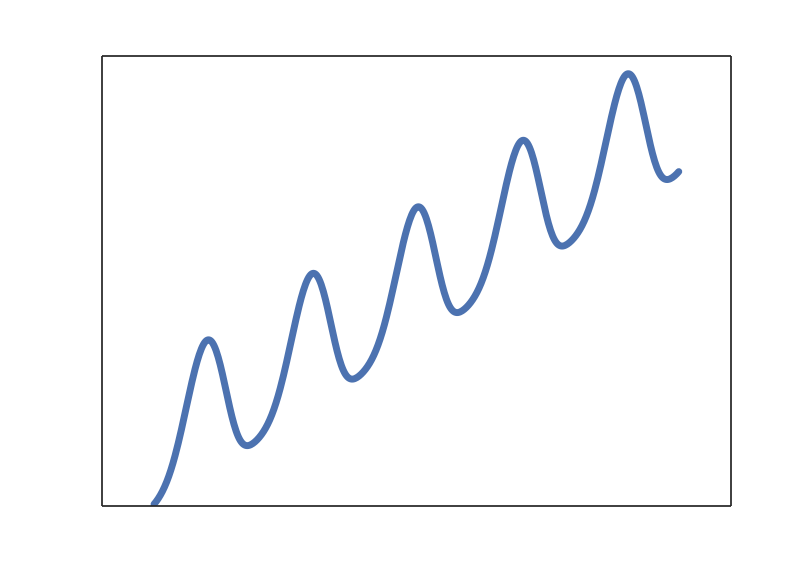
\includegraphics[height=2cm]{figs/kernel/kernelLINplusPER.png} & 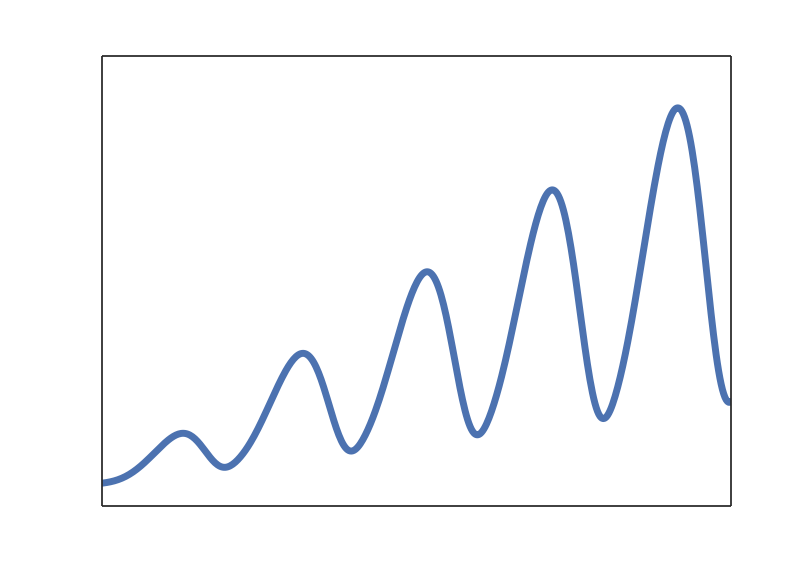
\includegraphics[height=2cm]{figs/kernel/kernelLINtimesPER.png} & 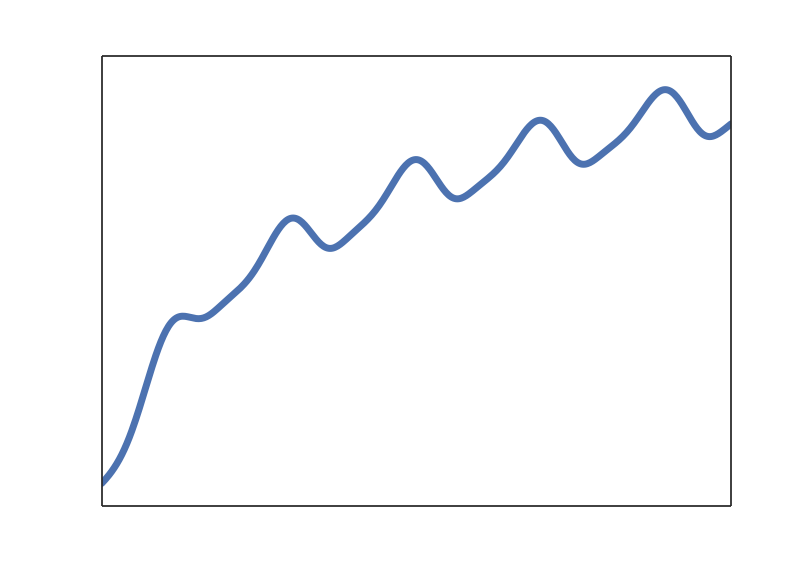
\includegraphics[height=2cm]{figs/kernel/kernelSEplusPER.png}& 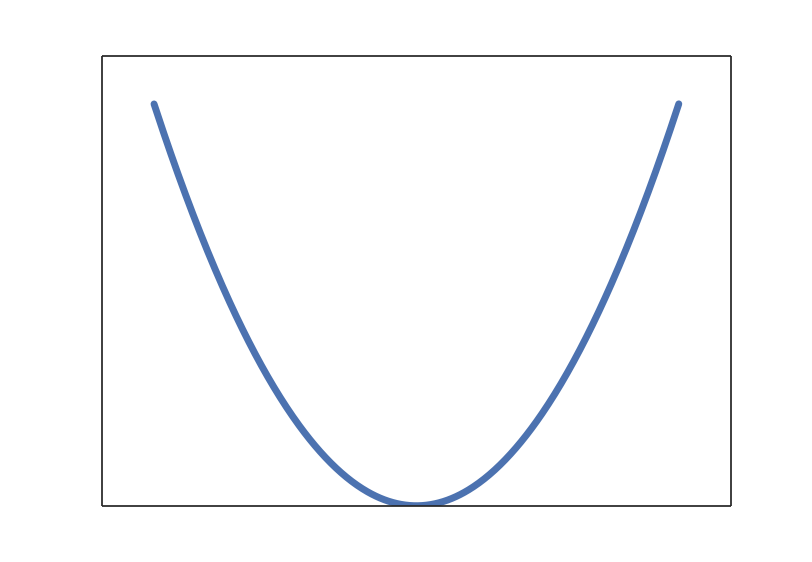
\includegraphics[height=2cm]{figs/kernel/kernelLINtimesLIN.png}\\
\end{tabular}
\caption{}
\end{subfigure}

\caption{(a) Graphical description of Bayesian GP structure learning. (b) Composite structure. (c) The natural language interpretation of the structure.}\label{fig:schema}
\end{figure}

The stochastic grammar models a prior on different structural compositions of the covariance function. An input of non-composite kernels (base kernels) is supplied to generate a posterior distributions of composite structure to express local and global aspects of the data.


We approximate the following intractable integrals of the expectation for the prediction:
\begin{equation}
\mathbb{E}[\hat{f} \mid \hat{x},\mathbf{D},\mathbf{K}] =\iint f(\hat{x},\bm{\theta},\mathbf{K})\,P(\bm{\theta} \mid \mathbf{D,\mathbf{K}})\,P(\mathbf{K}|\bm{\Omega},s,n) \; \mathbf{d} \bm{\theta} \mathbf{d} \mathbf{K}.  
\end{equation}

This is done by sampling from the posterior probability distribution of the hyper-parameters and the possible kernel:
\begin{equation}
\hat{f} \approx \frac{1}{T} \sum^T_{t=1} f(\hat{x} | \bm{\theta}^{(t)},\mathbf{K}^{(t)}). 
\end{equation}


In order to provide the sampling of the kernel, we introduce a stochastic process that simulates the grammar for algebraic expressions of covariance function algebra:
\begin{equation}
\mathbf{K}^{(t)} \sim  P(\mathbf{K} \mid \bm{\Omega},s,n)
\end{equation}
Here, we start with the set of given base kernels and draw a random subset.
For this subset of size $n$, we sample a set of possible operators $\bm{\Omega}$ combining base kernels. 
The marginal probability of a composite structure
\begin{equation}
P(\mathbf{K} \mid \bm{\Omega},s,n) = P(\bm{\Omega} \mid s,n)\times P(s \mid n) \times P(n),
\end{equation}
is characterized by the prior $P(n)$ on the number of base kernels used, the probability of a uniformly chosen subset of the set of $n$ possible covariance functions
\begin{equation}
\label{eq:subsets}
P(s \mid n) = \frac{n!}{ \mid s \mid !},
\end{equation}
and the probability of sampling a global or a local structure, which is given by a binomial distribution: 
\begin{equation}
P(\bm{\Omega} \mid s,n)= {n \choose r}  p_{+\times}^r (1 - p_{+\times})^{n-r}.
\end{equation}



Many equivalent covariance structures can be sampled due to covariance function algebra and equivalent representations with different parameterization~\citep{lloyd2014automatic}. To inspect the posterior of these equivalent structures we convert each kernel expression into a sum of products and subsequently simplify. All base kernels can be found in Appendix A, rules for this simplification can be found in appendix B. The code for learning of kernel structure is as follows:

\begin{mdframed}
\begin{minipage}{\linewidth}
\small
\belowcaptionskip=-10pt
\begin{lstlisting}[mathescape,label=alg:structureVent,basicstyle=\selectfont\ttfamily,numbers=none,escapechar=\#]
// GRAMMAR FOR KERNEL STRUCTURE
#\linenumber{1}#assume kernels = list(se, wn, lin, per, rq) // defined as above

// prior on the number of kernels
#\linenumber{2}#assume p_number_k = uniform_structure(n)
#\linenumber{3}#assume subset_kernels = tag(quote(grammar), 0,
#\linenumber{4}#                            subset(kernels, p_number_k))

// kernel composition
#\linenumber{5}#assume composition = proc(l) {
#\linenumber{6}#  if (size(l) <= 1) {
#\linenumber{7}#    first(l)
#\linenumber{8}#  } else {
#\linenumber{9}#    if (bernoulli()) {
#\linenumber{10}#      add_funcs(first(l), composition(rest(l)))
#\linenumber{11}#    } else {
#\linenumber{12}#       mult_funcs(first(l), composition(rest(l)))
#\linenumber{13}#    }
#\linenumber{14}#  }
#\linenumber{15}#}

#\linenumber{16}#assume K = tag(quote(grammar), 1, composition(subset_kernels))

// APPLY GPMEM
#\linenumber{17}#assume (f_compute, f_emu) = gpmem(f_look_up, K)

// Probe all data points
#\linenumber{18}#for n ... N
#\linenumber{19}#  predict f_compute(get_data_xs(n))

// PERFORMING INFERENCE
#\linenumber{20}#infer repeat(200, do(
#\linenumber{21}#  mh(quote(grammar), one, 1),
#\linenumber{22}#  for kernel in K:
#\linenumber{23}#    mh(quote(parameters$_{\text{kernel}}$), one, 1)))
\end{lstlisting}

\end{minipage}
\end{mdframed}


We defined a simmple space of covariance structures in a way that allows us to produce results coherent with 
work presented in Automatic Statistician. We illustrate results in Fig. \ref{fig:posterior} and \ref{fig:posterior_airline} using the Mauna Loa  CO$_2$ data set (see \citealp{rasmussen2006gaussian} for a description) and the airline data set describing monthly totals of international airline passengers (\citealp{box2011time}, according to \citealp{duvenaud2013structure}). Both datasets served as illustration in the Automatic Statistician project. Previous work on automated kernel discovery~\citep{duvenaud2013structure} illustrated the Mauna Loa data using an RQ kernel.
We resort to the white noise kernel instead RQ (similar to \citep{lloyd2014automatic}).

In contrast to what previous work has presented, we compute a posterior on structures. This allows us to gain valuable insight into the data that was previously unavailable. 
We can query the data for the probability of certain structures to hold true. For example, we could be interested in whether or not a trend as is present in the data.
We can also formulate queries using logical operators such as AND and OR. This provides us with a rich language to ask questions about our time series data and let the data speak for itself for finding the answers. We demonstrate this in Fig \ref{fig:query}.

\begin{figure}
\centering
 \addtolength\abovedisplayskip{-1\baselineskip}%
  \addtolength\belowdisplayskip{-1\baselineskip}%
 
\begin{tikzpicture}
\node (datatitle) {\small Raw Data};
\node[below = -0.25cm of datatitle] (data) {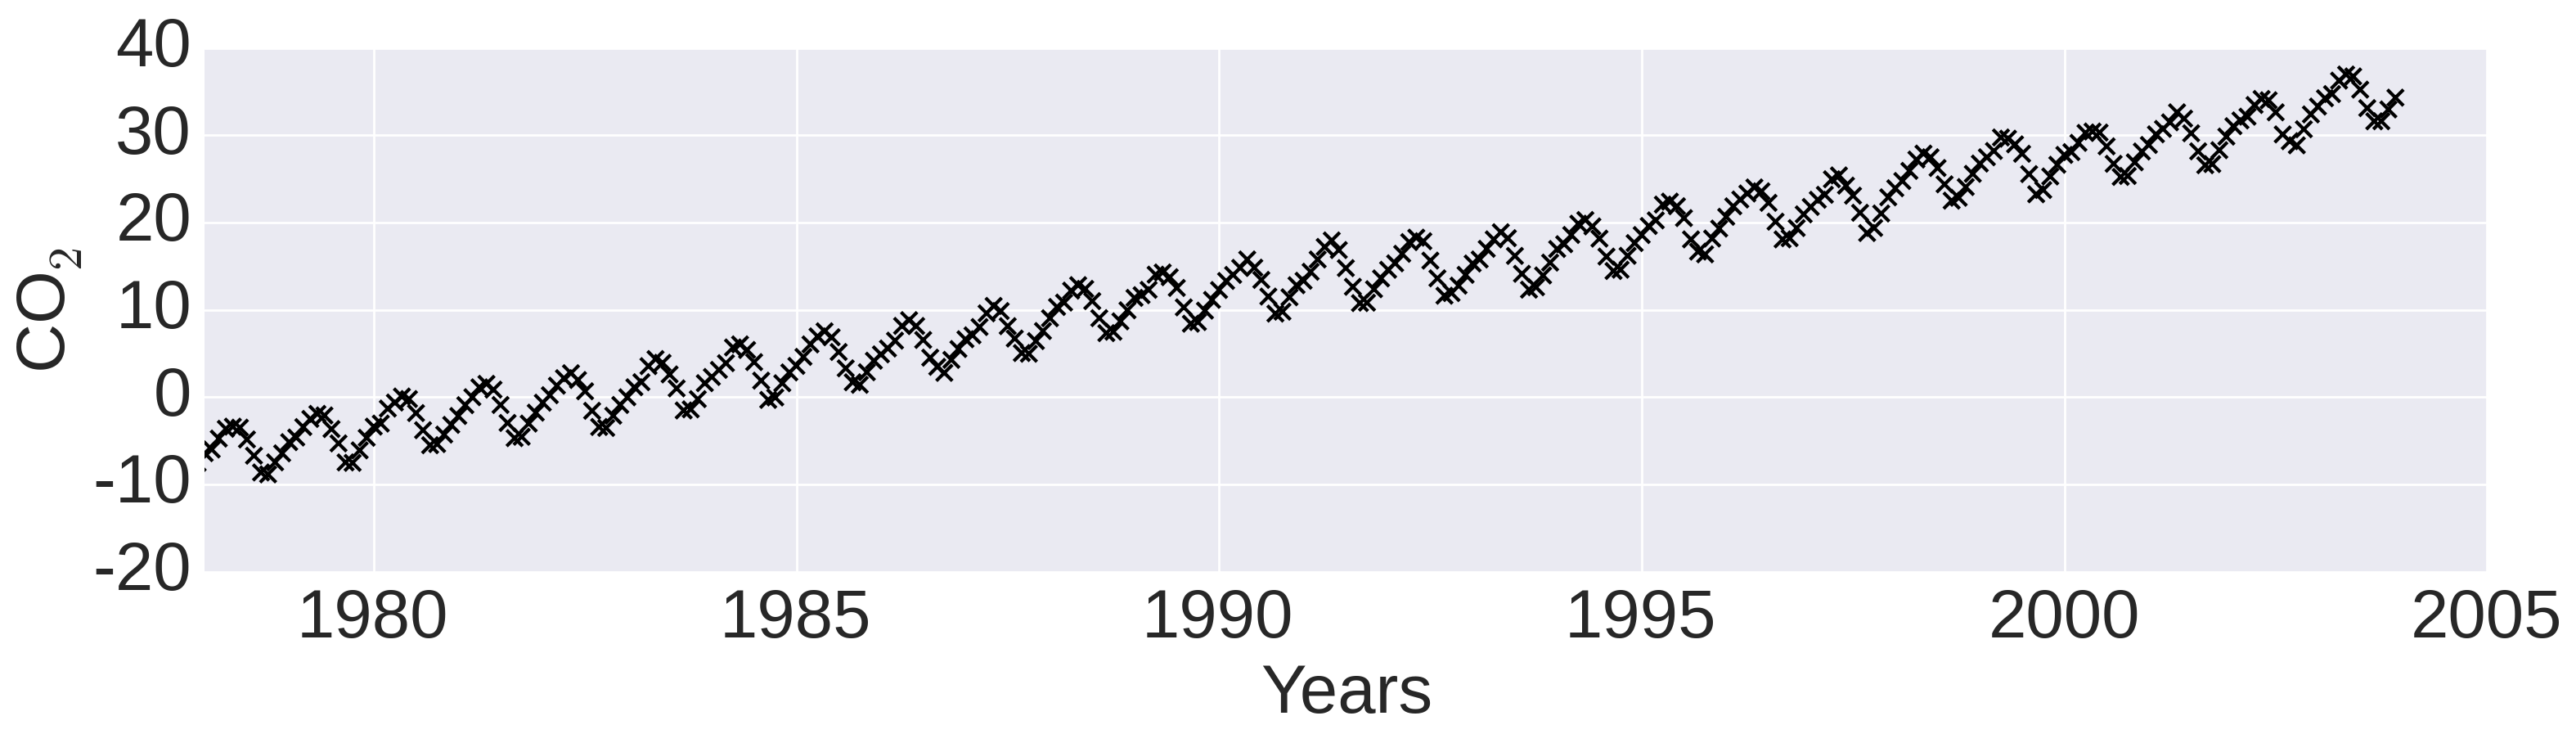
\includegraphics[width=0.7\textwidth]{figs/mauna_data.png}};
\node[below = 2.5cm of data] (post_param_helper) {};
\node[above = 1cm of post_param_helper] (post_param_helper_1) {};
\node[below = 1cm of post_param_helper] (post_param_helper_2) {};
\node[left = -3cm of post_param_helper] (post_param) {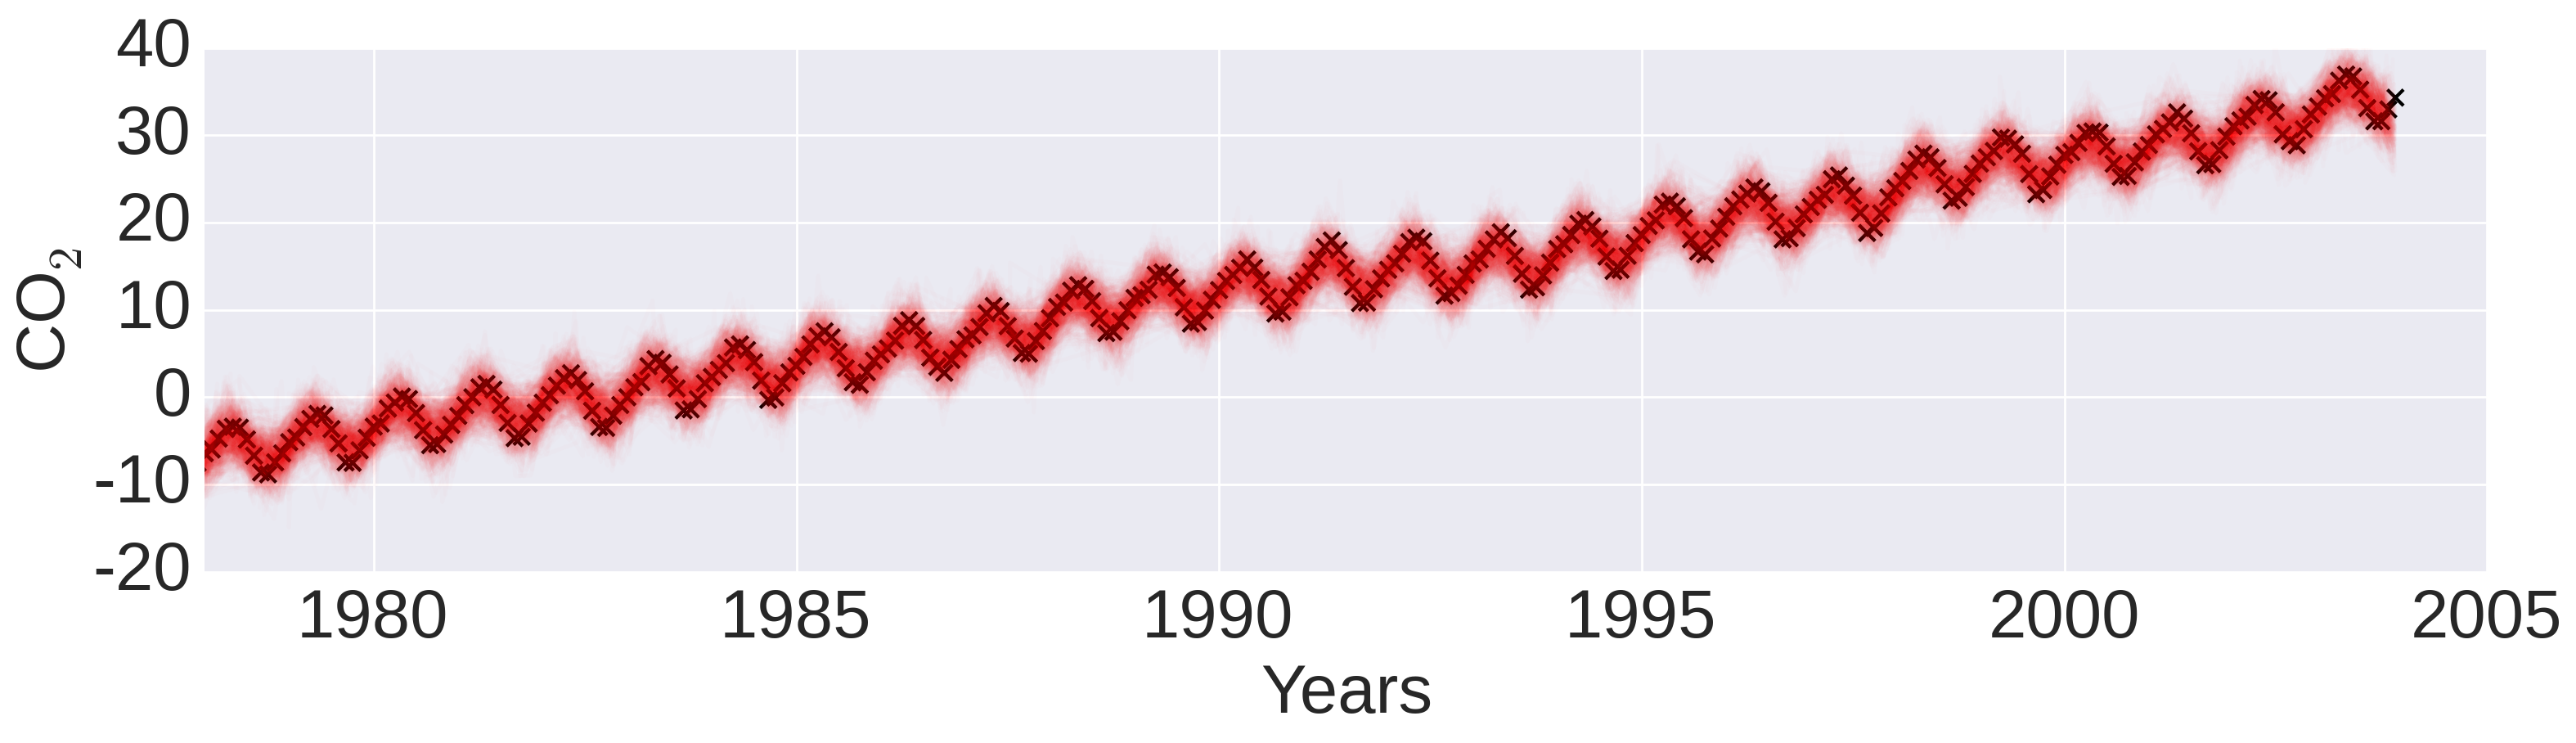
\includegraphics[width=0.6\textwidth]{figs/mauna_sample_1.png}};
\node[draw,rectangle,color=red,dashed,right = 4.5cm of post_param_helper,yshift=0.3cm] (zoom) {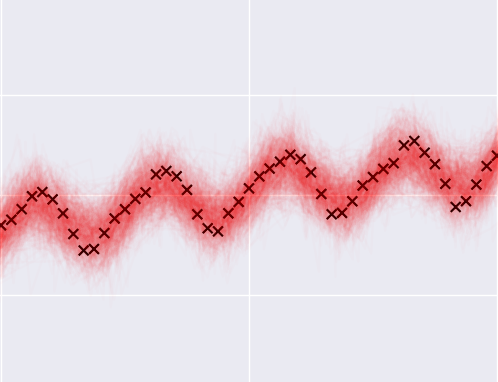
\includegraphics[width=0.2\textwidth]{figs/mauna_zoom.png}};
\node[draw,rectangle,color=red,dashed,left = 3.8cm of zoom, minimum width =
1.5cm, minimum height = 1.2cm,yshift=0.0cm] (zoom_in) {};
\node[below = 1.2cm of post_param_helper_2] (posterior) {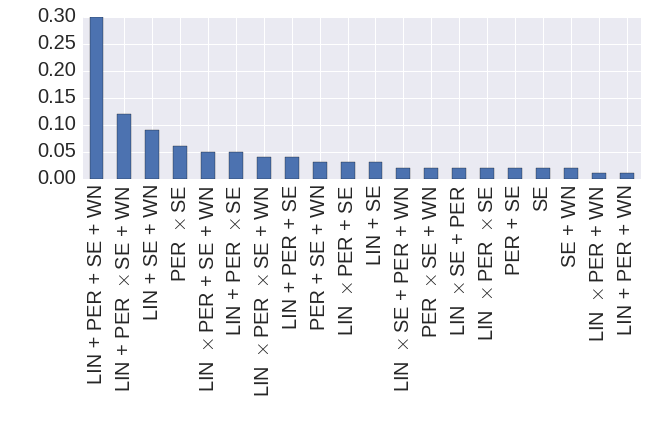
\includegraphics[width=0.6\textwidth]{figs/mauna_structure.png}};

\node[draw,rectangle,below = 1.2cm of posterior] (formula_param_1) {\color{black}\small
$\Ktheta= 2.7^2(x x^\prime) + 5.6^2 \exp \bigg( \frac{2 \sin^2 ( \pi (x - x^\prime)/3.7}{6.4^2} \bigg)
+ 0.4^2 \exp(-\frac{(x-x^\prime)^2}{2 \times 6.3^2}) +  1.9^2 \delta_{x,x^\prime} \label{eq:WN}$ };


\node[draw,rectangle,below = 1.2cm of formula_param_1,text width =
0.9\textwidth,minimum height = 1.5cm,font=\footnotesize] (paragraph){
The posterior peaks at a kernel structure with four additive components. Additive components hold globally, that is there are no higher level, qualitative aspects of the data that vary with the input space. The additive components are as follows: (i) a linearly increasing function or trend; (ii) a periodic function; (iii) a smooth function; and (iv) white noise.};







\node[draw, rectangle, left = -1.75cm of posterior,minimum width = 0.45cm, minimum height = 5.8cm,yshift=0.2cm] (mark_structure) {};
%\node[draw,very thick, rectangle, below = 1.1cm of data,minimum width = \textwidth, minimum height = 15cm] (posterior_frame) {};

%\node[left = 1.3cm of mark_structure] (paragraph_helper){};
\node[below =0.45cm of mark_structure,inner sep = 0pt,outer sep=0pt] (formula_helper) {};
\node[above =1.2cm of formula_param_1,inner sep = 0pt,outer sep=0pt] (formula_helper_2) {};

%\draw[-,dashed] (mark_structure.south) -- (formula_helper);
%\draw[-,dashed] (formula_helper) -- (formula_helper_2);
%\draw[->,dashed] (mark_structure) -- (paragraph_helper);
%\draw[->,dashed] (formula_helper_2) -- (formula);

\draw[->] (data) -- node[right]{\small $\hat \fbf \sim
\mathcal{N}(\hat{\bm{\mu}},\hat\Kbf)$} (post_param_helper_1);
\draw[->] (post_param_helper_2) -- node[right]{\small Posterior Structure} (posterior);
\draw[->] (formula_helper_2) -- node[right] {\small
$\bm{\theta}=\{2.7,5.6,3.7,6.4,0.4,6.3,1.9\}$} (formula_param_1);
\draw[-] (mark_structure) -- node[left, yshift=-0.3cm] {\small $\Ktheta$} (formula_helper);
\draw[-] (formula_helper) --(formula_helper_2);
\draw[->] (formula_param_1) -- node[right]{\small Qualitative Interpretation} (paragraph);

\draw[->,dashed,red] (zoom_in) --node[above]{\small\color{red}Zoom in:}
node[below]{\small\color{red}adequate error bars}(zoom);

%\draw[->,line width=1pt,double distance=2pt] (data) -- (post_param);
% starting from the bottom to aligm with caption 
\node[left=0.3cm of paragraph] (e){(e)}; 

\node[above=1.9cm of e] (d) {(d)}; 
\node[above=5.0cm of d] (c) {(c)}; 
\node[above=4.7cm of c] (b) {(b)}; 
\node[above=4.0cm of b] (a) {(a)}; 
\end{tikzpicture}
\addtolength\abovedisplayskip{1\baselineskip}%
\addtolength\belowdisplayskip{1\baselineskip}%



\caption{\small Posterior of structure and qualitative, human interpretable reading. We take the raw data (top), compute a posterior distribution on structures (red samples and bar plot).
We take the peak of this distribution ($\text{LIN}+\text{PER}+\text{SE}+\text{WN}$) with the sampled parameters used to generate the samples for the second plot from the top and write it in functional form with parameters. We depict the human readable interpretation of the equation on the bottom.}\label{fig:posterior}
\end{figure}

\begin{figure}
\centering
 \addtolength\abovedisplayskip{-1\baselineskip}%
  \addtolength\belowdisplayskip{-1\baselineskip}%
  
\begin{tikzpicture}
\node (datatitle) {\small Raw Data};
\node[below = -0.25cm of datatitle](data) {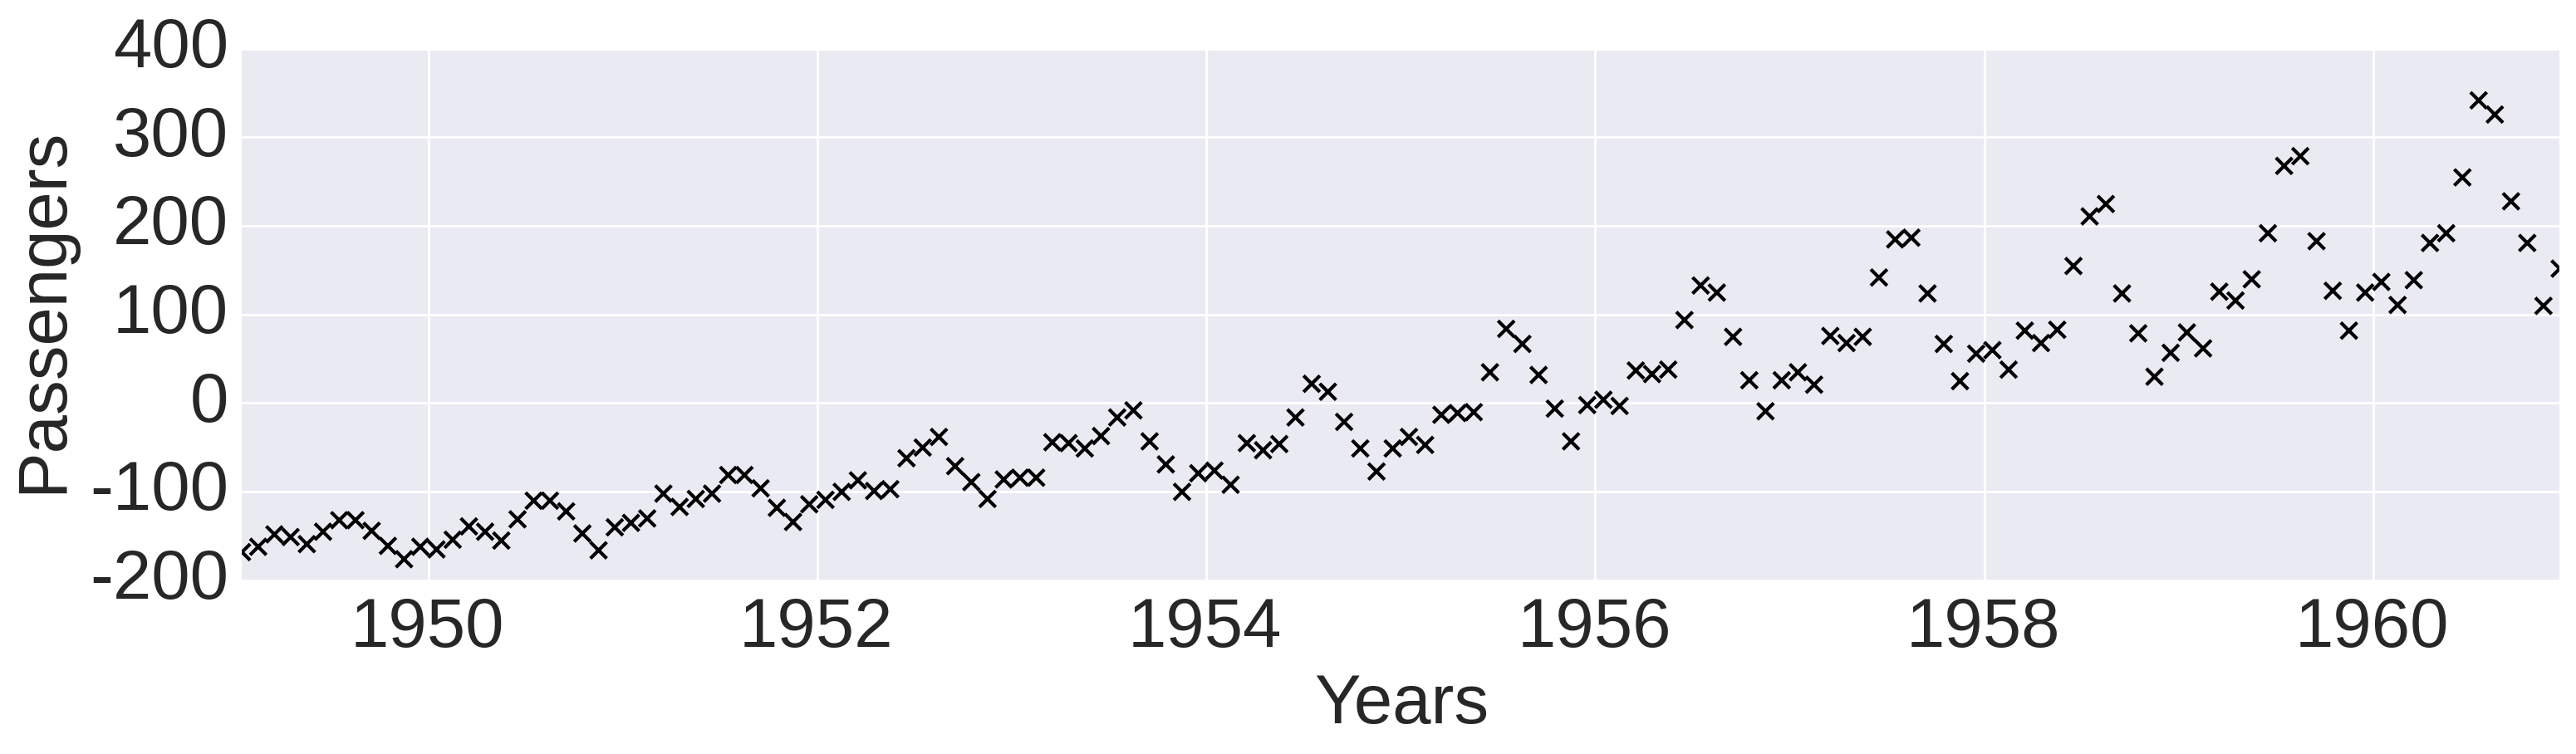
\includegraphics[width=0.65\textwidth]{figs/airline_data.png}};
\node[below= 1.2cm of data] (post_param) {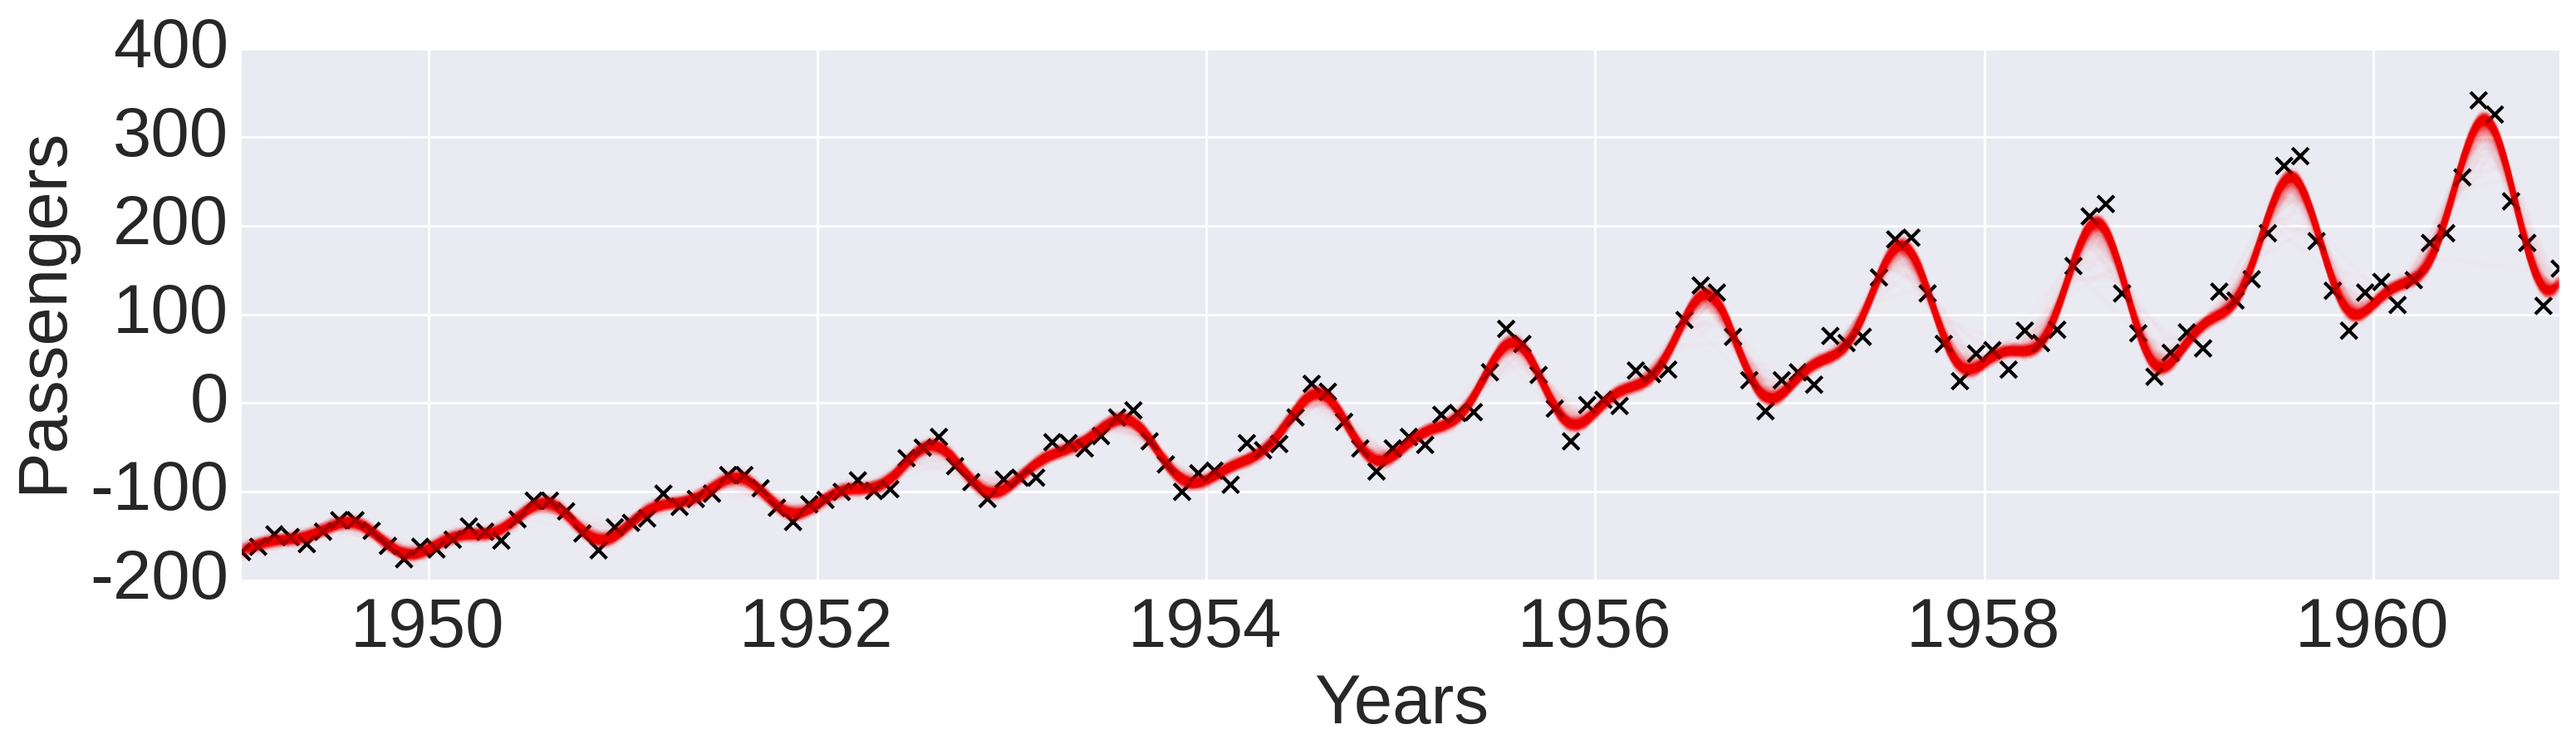
\includegraphics[width=0.65\textwidth]{figs/airline_sample_28.png}};


\node[below = 1.2cm of post_param] (posterior) {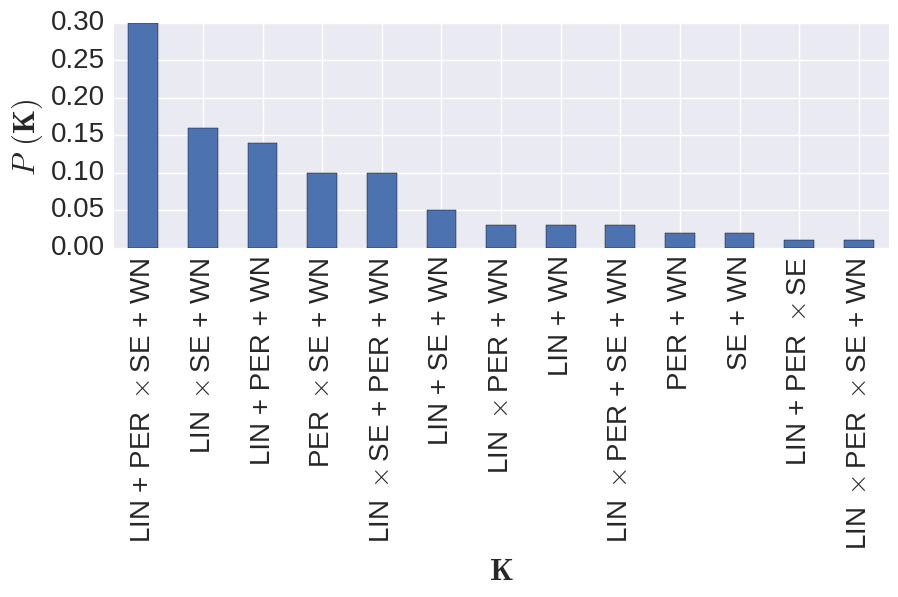
\includegraphics[width=0.55\textwidth]{figs/airline_structure.png}};
\node[below=-0.7cm of posterior,xshift=0.3cm] (xlabel) {\footnotesize
$\Ksrv$};
\node[left =-0.5cm of posterior,yshift=1.3cm] (ylabel) {\rotatebox{90}{\footnotesize
$P(\Ksrv \mid \xbf,\ybf, \thetabf )$}};
\node[draw,rectangle,below = 1.2cm of posterior] (formula_param_1) {\small\color{black}
$\ktheta= 7.47^2(x x^\prime) +
\Bigg(0.27^2 \exp(-\frac{(x-x^\prime)^2}{2 \times 4.63^2}) \times 
7.34^2 \exp \bigg( \frac{2 \sin^2 ( \pi (x - x^\prime)/4.4}{4.55^2} \bigg)\Bigg)
+ 2.93^2 \delta_{x,x^\prime} \label{eq:WN}$ };


\node[draw,rectangle,below = 1.2cm of formula_param_1,text width =0.9\textwidth,minimum height = 1.5cm, font=\footnotesize] (paragraph){ 
The posterior peaks at a kernel structure with three additive components.
Additive components hold globally, that is there are no higher level,
qualitative aspects of the data that vary with the input space. The additive
components are as follows: (i) a linearly increasing function or trend; (ii) an approximate periodic function; and (iv) white noise.};







\node[draw, rectangle, left = -1.7cm of posterior,minimum width = 0.45cm, minimum height = 5.2cm,yshift=0.2cm] (mark_structure) {};
%\node[draw,very thick, rectangle, below = 1.1cm of data,minimum width = \textwidth, minimum height = 15cm] (posterior_frame) {};

%\node[left = 1.3cm of mark_structure] (paragraph_helper){};
\node[below =0.45cm of mark_structure,inner sep = 0pt,outer sep=0pt] (formula_helper) {};
\node[above =1.2cm of formula_param_1,inner sep = 0pt,outer sep=0pt] (formula_helper_2) {};

%\draw[-,dashed] (mark_structure.south) -- (formula_helper);
%\draw[-,dashed] (formula_helper) -- (formula_helper_2);
%\draw[->,dashed] (mark_structure) -- (paragraph_helper);
%\draw[->,dashed] (formula_helper_2) -- (formula);

\draw[->] (data) -- node[right]{\small $\yprime \sim
\mathcal{N}(\mupost,\Kpost)$} (post_param_helper_1);
\draw[->] (post_param_helper_2) -- node[left]{\small }node[right]{\small Marginal on
Structure: $P(\Ksrv \mid \xbf,\ybf,\thetabf )$} (posterior);
\draw[->] (formula_helper_2) -- node[right] {\small
$\bm{\theta}=\{7.47,0.27,4.63,7.34,4.4,4.55,2.93\}$} (formula_param_1);
\draw[-] (mark_structure) -- node[left, yshift=-0.3cm] {\small $\ktheta$} (formula_helper);
\draw[-] (formula_helper) --(formula_helper_2);
\draw[->] (formula_param_1) -- node[right]{\small Qualitative Interpretation} (paragraph);


\node[left=0.3cm of paragraph] (e){(e)}; 

\node[above=1.9cm of e] (d) {(d)}; 
\node[above=5.0cm of d] (c) {(c)}; 
\node[above=4.7cm of c] (b) {(b)}; 
\node[above=4.0cm of b] (a) {(a)}; 
\end{tikzpicture}
\addtolength\abovedisplayskip{1\baselineskip}%
\addtolength\belowdisplayskip{1\baselineskip}%



\caption{\small Posterior of structure and qualitative, human interpretable reading. We take the raw data (top), compute a posterior distribution on structures (red samples and bar plot).
We take the peak of this distribution ($\text{LIN}+\text{PER} \times \text{SE}+\text{WN}$) with the sampled parameters used to generate the samples for the second plot from the top and write it in functional form with parameters. We depict the human readable interpretation of the equation on the bottom.}\label{fig:posterior_airline}
\end{figure}

\begin{figure}
\centering

% 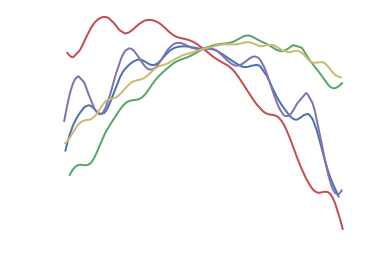
\includegraphics[width=.153\textwidth]{figs/gpSamples/main.png}
\begin{tikzpicture}


% level 1
\node (hyp) {\normalsize \color{blue} What is the probability of a trend, a recurring pattern {\bf and} noise in the data?};
\node[below = -0.2cm of hyp] (hyp_form) {$P\big((\text{LIN}\lor\text{LIN}\times\text{SE})\land
(\text{PER}\lor\text{PER}\times\text{SE}\lor\text{PER}\times\text{LIN})\land
(\text{WN}\lor\text{LIN}\times\text{WN})\big) = 0.36$};

%level 3
\node[below =.5cm of hyp_form , xshift=-3cm] (trend) {\color{blue} Is there a trend?};
\node[below = -0.2cm of trend] (trend_form) {$P(\text{LIN}\lor\text{LIN}\times\text{SE}) = 0.65$};
\node[below = -0.2cm of trend_form] (trend_png) {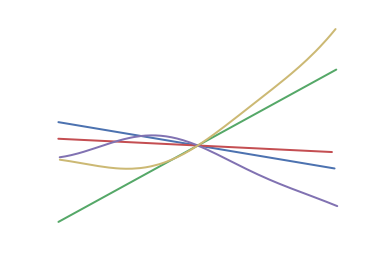
\includegraphics[width=.15\textwidth]{figs/gpSamples/trend.png}};

\node[below =.5cm of hyp_form, xshift=3cm] (noise) {\color{blue} Is there noise? };
\node[below = -0.2cm of noise] (noise_form) {$P(\text{WN}\lor\text{LIN}\times\text{WN}) = 0.75$};
\node[below = -0.2cm of noise_form] (noise_png) {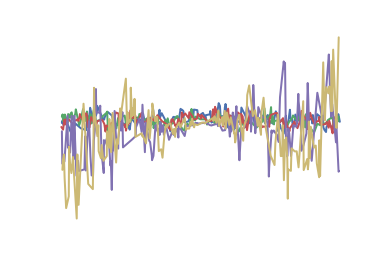
\includegraphics[width=.15\textwidth]{figs/gpSamples/noise.png}};

% level 4
\node[below =.5cm of trend_png , xshift=-2cm] (linear_trend) {\color{blue} A linear trend?};
\node[below = -0.2cm of linear_trend] (linear_trend_form) {$P(\text{LIN}) = 0.63$};
\node[below = -0.2cm of linear_trend_form] (linear_trend_png) {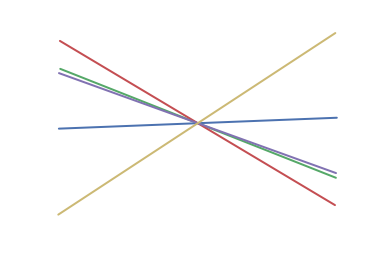
\includegraphics[width=.15\textwidth]{figs/gpSamples/lin.png}};

\node[below =.5cm of trend_png , xshift=1cm] (smooth_trend) {\color{blue} A smooth trend?};
\node[below = -0.2cm of smooth_trend] (smooth_trend_form) {$P(\text{LIN}\times\text{SE}) = 0.02$};
\node[below = -0.2cm of smooth_trend_form] (smooth_trend_png) {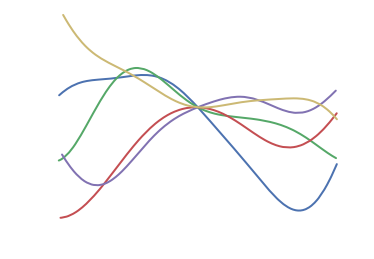
\includegraphics[width=.15\textwidth]{figs/gpSamples/selin.png}};

\node[below =.5cm of noise_png, xshift=-1cm] (het_noise) {\color{blue} Heteroskedastic noise? };
\node[below = -0.2cm of het_noise] (het_noise_form) {$P(\text{LIN}\times\text{WN}) = 0$};
\node[below = -0.2cm of het_noise_form] (het_noise_png) {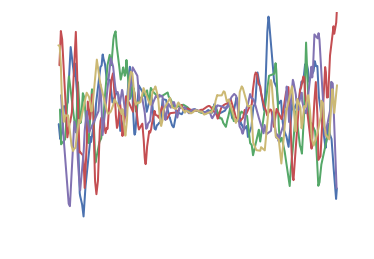
\includegraphics[width=.15\textwidth]{figs/gpSamples/linwn.png}};

\node[below =.5cm of noise_png, xshift=2cm] (white_noise) {\color{blue} White  noise? };
\node[below = -0.2cm of white_noise] (white_noise_form) {$P(\text{WN}) = 0.75$};
\node[below = -0.2cm of white_noise_form] (white_noise_png) {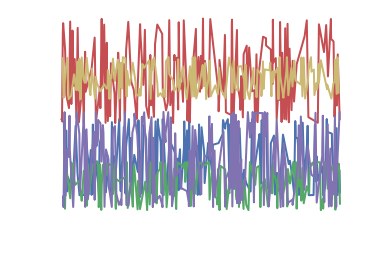
\includegraphics[width=.15\textwidth]{figs/gpSamples/wn.png}};

% level 5
\node[below =6.2cm of hyp_form] (recurring) {\color{blue} Is there repeating structure?};
\node[below = -0.2cm of recurring] (recurring_form) {$P(\text{PER}\lor\text{PER}\times\text{SE}\lor\text{PER}\times\text{LIN}) = 0.73$};
\node[below = -0.2cm of recurring_form] (recurring_png) {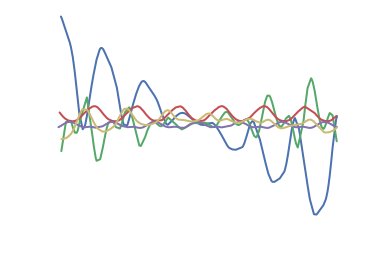
\includegraphics[width=.15\textwidth]{figs/gpSamples/recurring.png}};
%\draw[->,dashed] (barplot) -- (mcmc);

% level 6
\node[below =.5cm of recurring_png] (seper_form) {$\text{PER}\times\text{SE}=0.34$};
\node[below = -0.2cm of seper_form] (seper_png) {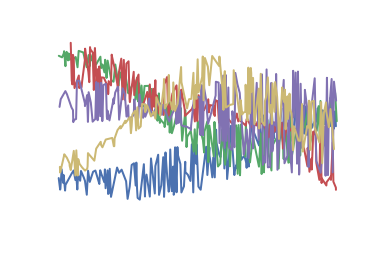
\includegraphics[width=.15\textwidth]{figs/gpSamples/seper.png}};

\node[below =.5cm of recurring_png, xshift=-3cm] (per_form) {$\text{PER}=0.32$};
\node[below = -0.2cm of per_form] (per_png) {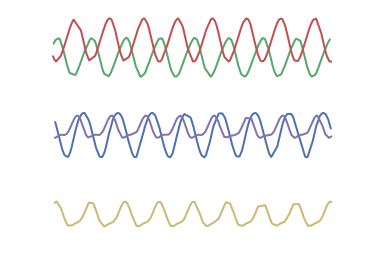
\includegraphics[width=.15\textwidth]{figs/gpSamples/per.png}};

\node[below =.5cm of recurring_png,xshift=3cm] (perlin_form) {$\text{PER}\times\text{LIN}=0.07$};
\node[below = -0.2cm of perlin_form] (seper_png) {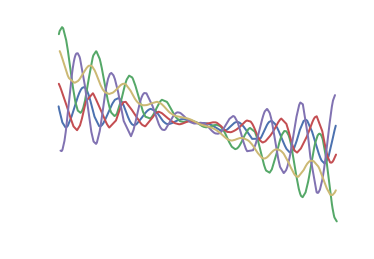
\includegraphics[width=.15\textwidth]{figs/gpSamples/perlin.png}};





\draw[->] (hyp_form) -- (trend);
\draw[->] (hyp_form) -- (noise);
\draw[->] (hyp_form) -- (recurring);


\draw[->] (noise_png) -- (het_noise);
\draw[->] (noise_png) -- (white_noise);

\draw[->] (trend_png) -- (linear_trend);
\draw[->] (trend_png) -- (smooth_trend);

\draw[->] (recurring_png) -- (per_form);
\draw[->] (recurring_png) -- (seper_form);
\draw[->] (recurring_png) -- (perlin_form);


\end{tikzpicture}



%  \multicolumn{3}{c}{$P(\text{PER}\lor\text{PER}\times\text{SE}\lor\text{PER}\times\text{LIN})$}

\caption{We can query the data if some logical statements are probable to be true, for example, is it true that there is a trend?}\label{fig:query}
\end{figure}

\FloatBarrier
\section{Bayesian Optimization}
\label{sec:bayesopt}
Bayesian optimization casts the problem of finding the global maximum of an unknown function as a hierarchical decision problem~\citep{ghahramani2015probabilistic}.
Evaluating the actual function may be very expensive, either in computation time or in some other resource.
For one example, when searching for the best configuration for the learning algorithm of a large convolutional neural network, a large amount of computational work is required to evaluate a candidate configuration, and the space of possible configurations is high-dimensional.
Another common example, alluded to in Section \ref{sec:gpmem-broader}, is data acquisition: for machine learning problems in which a large body of data is available, it is often desirable to choose the right queries to produce a data set on which learning will be most effective.
In continuous settings, many Bayesian optimization methods employ GPs~\citep[e.g.][]{snoek2012practical}.

We have implemented a version of Thompson sampling using GPs in Venture.
Thompson sampling~\cite{thompson1933likelihood} is a widely-used Bayesian framework for solving exploration-exploitation problems.
Our implementation has two notable features: (i) the ability to search over a broader space of contexts than the parametric families that are typically used, and (ii) the parsimony of the resulting probabilistic program.


\subsection{Thompson sampling framework}
We now lay out the setup of Thompson sampling for Markov decision processes (MDPs).
An agent is to take a sequence of actions $a_1, a_2, \ldots$ from a (possibly infinite) set of possible actions $\Acal$.
After each action, a reward $r \in \R$ is received, according to an unknown conditional distribution $P_\true(r|a)$.
The agent's goal is to maximize the total reward received for all actions.
In Thompson sampling, the Bayesian agent accomplishes this by placing a prior distribution $P(\theta)$ on the possible ``contexts'' $\theta \in \Theta$.
Here a context is a believed model of the conditional distributions $\{P(r|a)\}_{a \in \Acal}$, or at least, a believed statistic of these conditional distributions which is sufficient for deciding an action $a$.
One example of such a sufficient statistic is the conditional mean $V(a|\theta) = \Ebkt{r|a,\theta}$, which can be thought of as a value function.
Thompson sampling thus has the following steps, repeated as long as desired:
\begin{enumerate}
  \item Sample a context $\theta \sim P(\theta)$.
  \item Choose an action $a \in \Acal$ which (approximately) maximizes $V(a|\theta) = \Ebkt{r|a,\theta}$.
  \item\label{itm:Thompson-conditioning}
    Let $r_\true$ be the reward received for action $a$.
    Update the believed distribution on $\theta$, i.e., $P(\theta) \gets P_\rmnew(\theta)$ where $P_\rmnew(\theta) = P\pn{\theta \mvert a \mapsto r_\true}$.
\end{enumerate}
Note that when $\Ebkt{r|a,\theta}$ (under the sampled value of $\theta$ for some points $a$) is far from the true value $\Ebkt[P_\true]{r|a}$, the chosen action $a$ may be far from optimal, but the information gained by probing action $a$ will improve the belief $\theta$.
This amounts to ``exploration.''
When $\Ebkt{r|a,\theta}$ is close to the true value except at points $a$ for which $\Ebkt{r|a,\theta}$ is low, exploration will be less likely to occur, but the chosen actions $a$ will tend to receive high rewards.
This amounts to ``exploitation.''
Roughly speaking, exploration will happen until the context $\theta$ is reasonably sure that the unexplored actions are probably not optimal, at which time the sampler will exploit by choosing actions in regions it knows to have high value.

Typically, when Thompson sampling is implemented, the search over contexts $\theta \in \Theta$ is limited by the choice of representation.
In traditional programming environments, $\theta$ often consists of a few numerical parameters for a family of distributions of a fixed functional form.
With work, a mixture of a few functional forms is possible; but without probabilistic programming machinery, implementing a rich context space $\Theta$ would be an unworkably large technical burden.
In a probabilstic programing language, however, the representation of heterogeneously structured or infinite-dimensional context spaces is quite natural.
Any computable model of the conditional distributions $\br{P(r|a)}_{a \in \Acal}$ can be represented as a stochastic procedure $(\lambda (a) \ldots)$.
Thus, for computational Thompson sampling, the most general context space $\widehat\Theta$ is the space of program texts.
Any other context space $\Theta$ has a natural embedding as a subset of $\widehat\Theta$.


\subsection{Thompson sampling in Venture}

Because Venture supports sampling and inference on (stochastic-)procedure-valued random variables (and the generative models which produce those procedures), Venture can capture arbitrary context spaces as described above.
To demonstrate, we have implemented Thompson sampling in Venture in which the contexts $\theta$ are Gaussian processes over the action space $\Acal = \R$.
That is, $\theta = (\mu, K)$, where the mean $\mu$ is a computable function $\Acal \to \R$ and the covariance $K$ is a computable (symmetric, positive-semidefinite) function $\Acal \times \Acal \to \R$.
This represents a Gaussian process $\br{R_a}_{a \in \Acal}$, where $R_a$ represents the reward for action $a$.
% where for any finite subset $\br{a_i}_{i=1}^{n} \subset \Acal$, the marginal distribution on $\pn{R_{a_i}}$ is Gaussian with mean $\pn{\mu(a_i)}_{i=1}^{n}$ and covariance matrix $\begin{pmatrix} K(a_i,a_j) \end{pmatrix}_{1 \leq i,j \leq n}$.
Computationally, we represent a context not as a pair of infinite lookup tables for $\mu$ and $K$, but as a finite data structure $\theta = (K_\prior, \sigma, \ell, \abf_\past, \rbf_\past)$, where
\begin{itemize}
  \item $K_\prior = K_{\prior,\sigma,\ell}$ is a procedure, with parameters $\sigma,\ell$, to be used as the prior covariance function: $K_\prior(a,a') = \sigma^2 \exp\pn{-\frac{(a-a')^2}{2\ell^2}}$
  \item $\sigma$ and $\ell$ are (hyper)parameters for $K_\prior$
  \item $\abf_\past = \pn{a_i}_{i=1}^{n}$ are the previously probed actions
  \item $\rbf_\past = \pn{r_i}_{i=1}^{n}$ are the corresponding rewards
\end{itemize}
To simplify the treatment, we take prior mean $\mu_\prior \equiv 0$.  The mean and covariance for $\theta$ are then gotten by the usual conditioning formula:
\begin{align*}
  \mu(\abf)
  &= \mu\pn{\abf \mvert \abf_\past, \rbf_\past} \\
  &= K_\prior(\abf, \abf_\past)
     \,K_\prior(\abf_\past, \abf_\past)^{-1}
     \,\rbf_\past \\
  K(\abf, \abf)
  &= K\pn{\abf, \abf \mvert \abf_\past, \rbf_\past} \\
  &= K_\prior(\abf, \abf)
     - K_\prior(\abf, \abf_\past)
       \,K_\prior(\abf_\past, \abf_\past)^{-1}
       \,K_\prior(\abf_\past, \abf).
\end{align*}
Note that even in this simple example, the context space $\Theta$ is not a finite-dimensional parametric family, since the vectors $\abf_\past$ and $\rbf_\past$ grow as more samples are taken.
$\Theta$ is, however, quite easily representable as a computational procedure together with parameters and past samples, as we do in the representation $\theta = (K_\prior, \sigma, \ell, \abf_\past, \rbf_\past)$.


\subsection{Implementation with \gpmem}

As a demonstration, we use Thompson sampling to optimize an unknown function $V(x)$ (the value function) using \gpmem.
(\textbf{TODO} we should not assume $V$ is deterministic, it would be easy enough to make it random or have it give noisy samples.)
We assume $V$ is made available to Venture as a black-box.
The code for optimizing $V$ is given in Listing \ref{alg:bayesopt}.
For step \ref{itm:Thompson-conditioning} of Thompson sampling, the Bayesian update, we not only condition on the new data (the chosen action $a$ and the received reward $r$), but also perform inference on the hyperparameters $\sigma, \ell$ using a Metropolis--Hastings sampler.
These two inference steps take 1 line of code: 0 lines to condition on the new data (as this is done automatically by \gpmem), and 1 line to call Venture's built-in \texttt{MH} operator.
The results are shown in Figure \ref{fig:bayesopt-sequence}.
We can see from the figure that, roughly speaking, each successive probe point $a$ is chosen either because the current model $V_\emu$ thinks it will have a high reward, or because the value of $V_\emu(a)$ has high uncertainty.
In the latter case, probing at $a$ decreases this uncertainty and, due to the smoothing kernel, also decreases the uncertainty at points near $a$.
We thus see that our Thompson sampler simultaneously learns the value function and optimizes it.

\begin{minipage}{\linewidth}
\small
\belowcaptionskip=-10pt
\begin{lstlisting}[frame=single,caption={
  Code for Bayesian optimization using \gpmem.
  %The procedure \texttt{V\_compute} probes \texttt{V} directly, thus improving the GP model \texttt{V\_emu}.
  %(\texttt{V\_emu\_pointwise} is simply a shortcut for sampling the GP model at a single point; \texttt{V\_emu} is more general, allowing joint samples to be taken at any set of points.)
  In the loop, \texttt{V\_compute} is called to probe the value of \texttt{V} at a new argument.
  The new argument, \texttt{(mc\_argmax V\_emu\_pointwise mc\_sampler)}, is a Monte Carlo estimate of the maximum pointwise sample of \texttt{V\_emu} (itself a stochastic quantity), with the Monte Carlo samples being drawn in this case uniformly between $-20$ and $20$.
  After each new call to \texttt{V\_compute}, the Metropolis--Hastings algorithm is used to perform inference on the hyperparameters of the covariance function in the GP model in light of the new conditioning data.
  Once enough calls to \texttt{V\_compute} have been made (in our case we stopped at 15 calls), we can inspect the full list of probed $(a,r)$ pairs with \texttt{extract\_stats}.
  The answer to our maximization problem is simply the pair having the highest $r$; but our algorithm also learns more potentially useful information.},mathescape,label=alg:bayesopt]
assume log_sf = tag('hyper, log(uniform_continuous(0, 10)))
assume log_l = tag('hyper, log(uniform_continuous(0, 10)))
assume se = make_squaredexp(log_sf, log_l)
assume blackbox_f = get_bayesopt_blackbox()
assume (f_compute, f_emu) = gpmem(blackbox_f, se)

define get_uniform_candidate = proc(prev_xs) {
  uniform_continuous(-20, 20)
}

define mc_argmax = proc(func, prev_xs) {
  // Monte Carlo estimator for the argmax of func.
  run(do(
    candidate_xs <- mapv(proc(i) {get_uniform_candidate(prev_xs)},
                         linspace(0, 19, 20)),
    candidate_ys <- mapv(func, candidate_xs),
    lookup(candidate_xs, argmax_of_array(candidate_ys))))
}

define emulator_point_sample = proc(x) {
  run(sample(lookup(
    f_emu(array(x)),
    0)))
}

infer repeat(15, do(pass,
     // Phase 2: Call f_compute on the next probe point
     predict f_compute(
                 mc_argmax(emulator_point_sample, '_)),
     // Phase 1: Hyperparameter inference
     mh('hyper, one, 50)))
\end{lstlisting}
\end{minipage}
      
\begin{figure}
\centering
    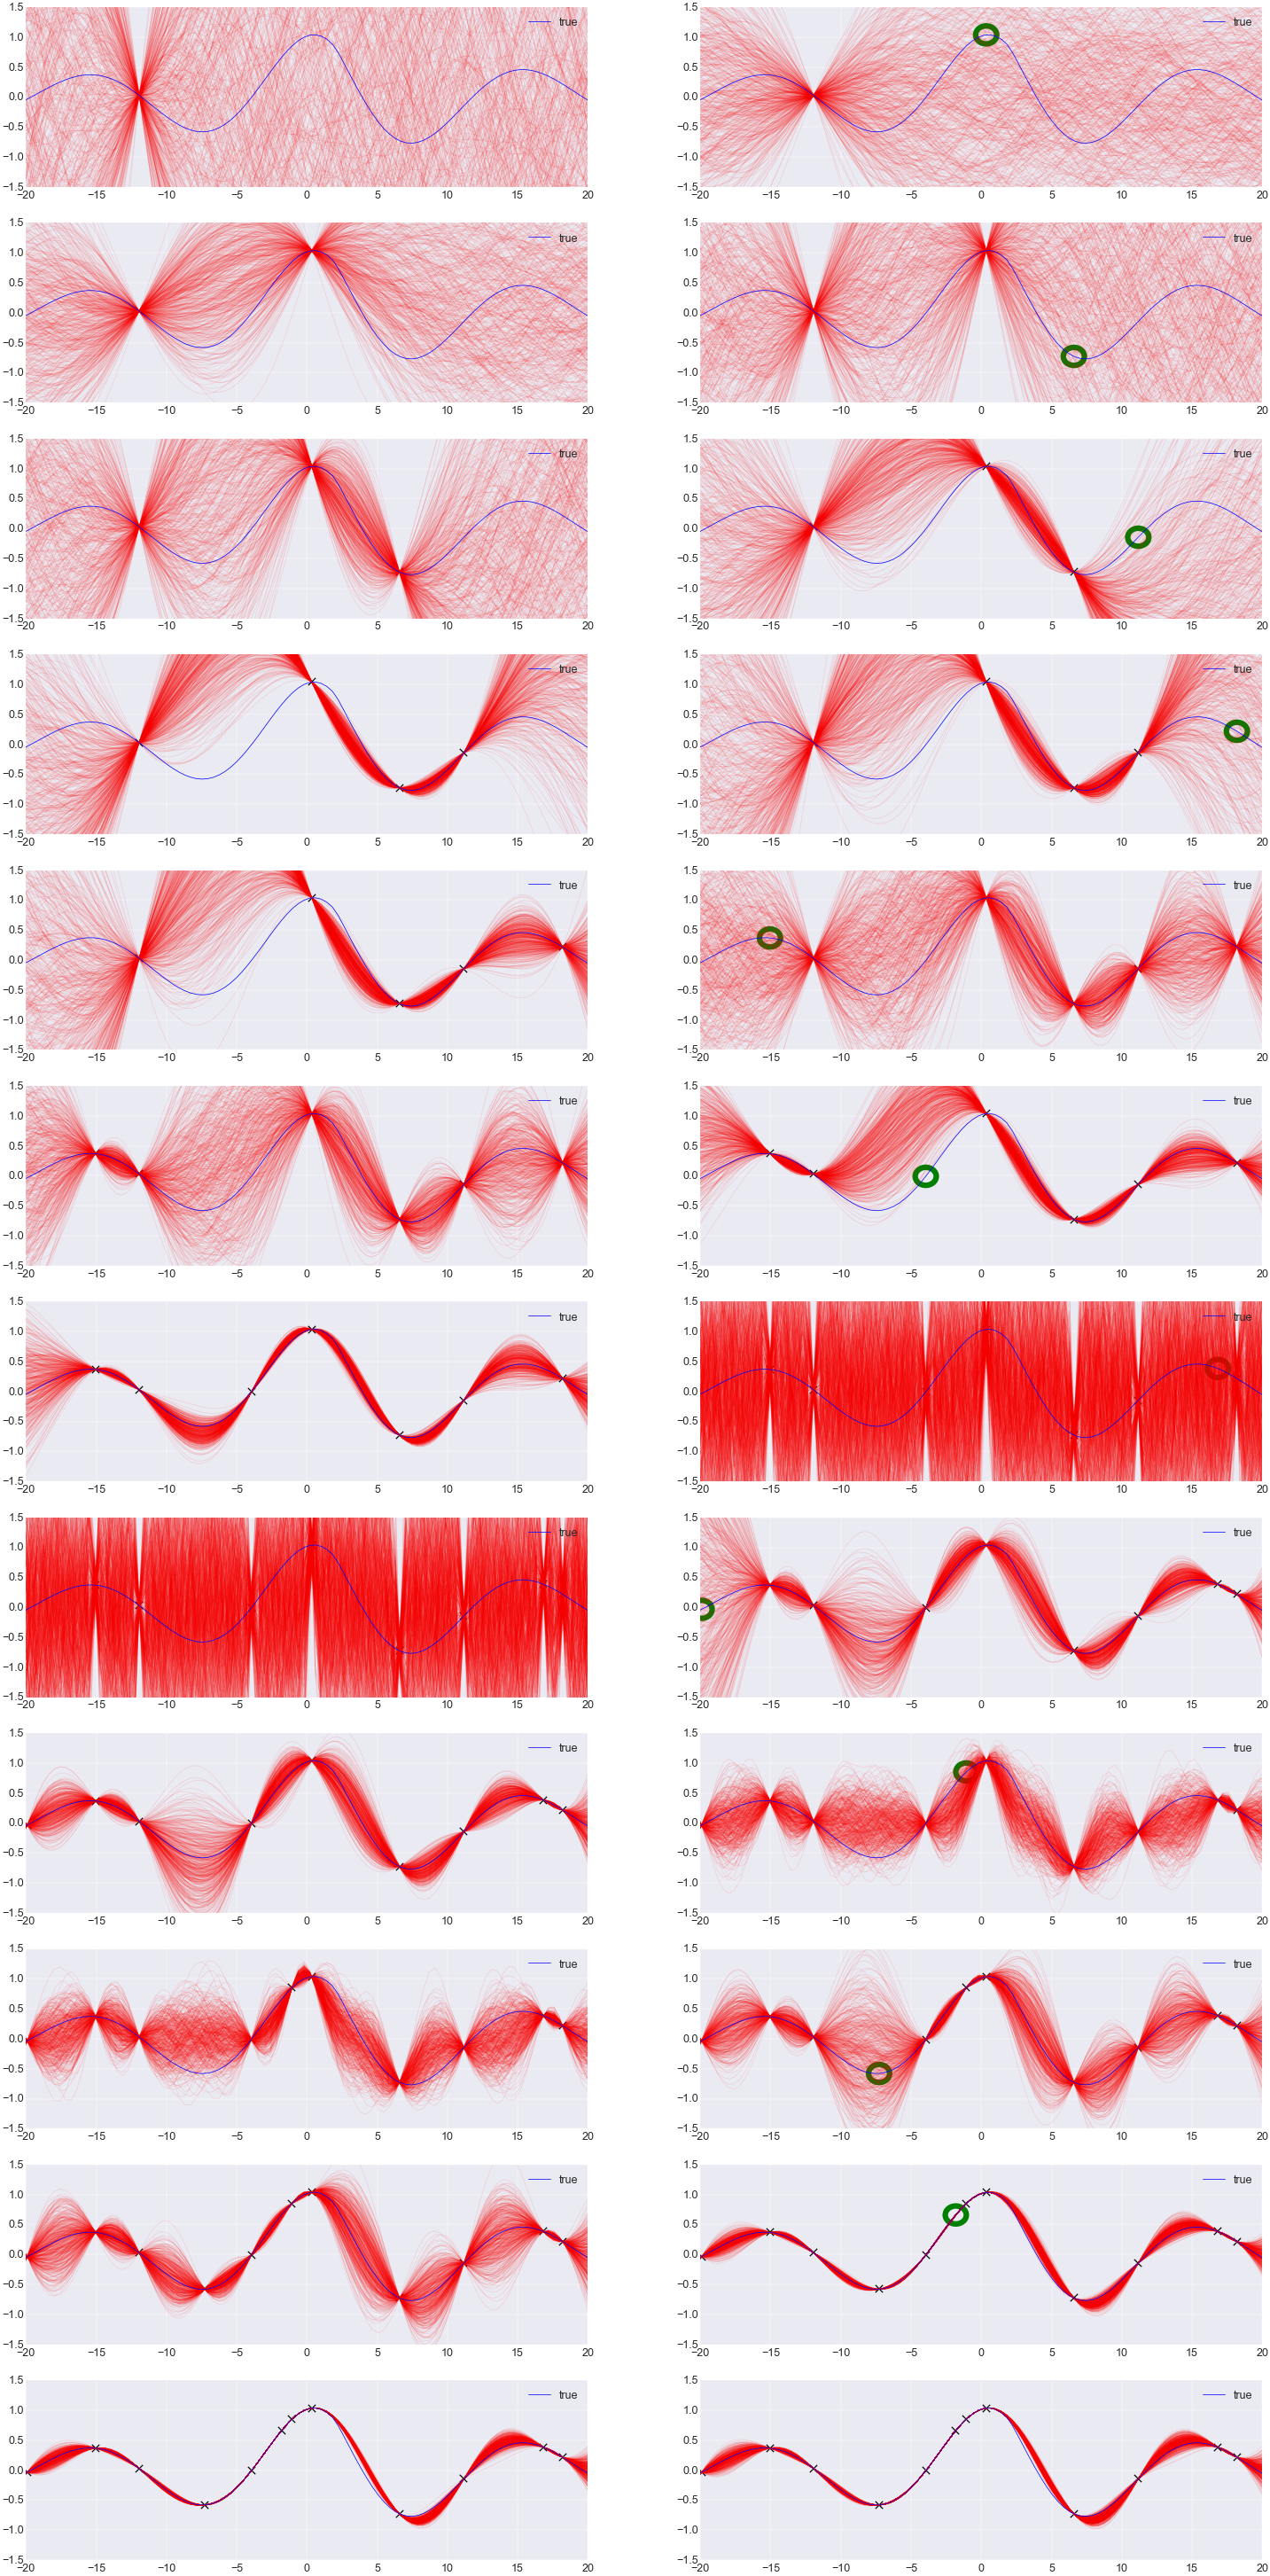
\includegraphics[height=0.8\textheight]{figs/BayesOpt_gpmem_sequence.png}
    \caption{
      Dynamics of Thompson sampling in Venture.
      The blue curve is the true function $V$, and the red region is a blending of 100 samples of the curve generated (jointly) by a GP-based emulator $V_\emu$.
      The left and right columns show the state of $V_\emu$ before and after hyperparameter inference is run on the new data, respectively.
      (We can see, for example, that after the seventh probe point, the Metropolis--Hastings sampler chose a ``crazy'' set of hyperparameters, which was corrected at the next inference step.)
      In the right column, the next chosen probe point is circled in green.
      Each successive probe point $a$ is the (stochastic) maximum of $V_\emu$, sampled pointwise and conditioned on the values of the previously probed points.
      Note that probes tend to happen at points either where the value of $V_\emu$ is high, or where $V_\emu$ has high uncertainty.
      }
    \label{fig:bayesopt-sequence}
\end{figure}



%We consider a true and  unknown reward function $r(x)$ that we estimate with a GP prior $\mathcal{GP}(0,K(\mathbf{x},\mathbf{x}))$. We denote past observations with $\mathcal{D} = \{(x;

\FloatBarrier

\section{Conclusion}
This paper has shown that it is feasible and useful to embed Gaussian processes
in higher-order probabilistic programming languages by treating them as a kind
of statistical memoizer. It has described classic GP regression with both fully
Bayesian and MAP inference in a hierarchical hyperprior, as well as state-of-the-art
applications to discovering symbolic structure in time series and to Bayesian optimization.
All the applications share a common 50-line Python GP library and require fewer than 20 lines
of probabilistic code each.

These results suggest several research directions. First, it will be important
to develop versions of {\tt gpmem} that are optimized for larger-scale
applications. Possible approaches include the standard low-rank approximations
to the kernel matrix that are popular in machine learning~\citep{bui2014tree} as well
as more sophisticated sampling algorithms for approximate conditioning of the
GP~\citep{lawrence2009efficient}.
Second, it seems fruitful to abstract the notion of a ``generalizing" memoizer
from the specific choice of a Gaussian process model as the mechanism for
generalization. ``Generalizing" or statistical memoizers with custom regression techniques could be broadly useful in performance engineering and scheduling systems.
The timing data from performance benchmarks could be run through a generalizing memoizer by default.
This memoizer could be queried (and its output error bars examined) to inform the best strategy
for performing the computation or predict the likely runtime of long-running jobs.
 Third, the structure learning application suggests follow-on research in information
retrieval for structured data. It should be possible to build a time series search engine
that can handle search predicates such as ``has a rising trend starting around
1988" or ``is perodic during the 1990s".
The variation on the Automated Statistician presented in this paper can provide ranked result
sets for these sorts of queries because it tracks posterior uncertainty over structure and also
because the space of structural patterns that it can handle is easy to modify by making small
changes to a short VentureScript program.


The field of Bayesian nonparametrics offers a principled, fully Bayesian
response to the empirical modeling philosophy in machine learning~\citep{ghahramani2013bayesian},
where Bayesian inference is used to encode a state of broad ignorance rather
than a bias stemming from strong prior knowledge. It is perhaps surprising that
two key objects from Bayesian nonparametrics, Dirichlet processes and Gaussian
processes, fit naturally in probabilistic programming as variants of
memoization~\citep{roy2008stochastic}. It is not yet clear if the same will be true
for other processes, e.g. Wishart processes, or hierarchical Beta processes. We hope that the results in this paper encourage the development of other nonparametric libraries for higher-order probabilistic programming languages.


\section*{Appendix}
\subsection*{A Covariance Functions}
\begin{align}
&\kse &=& \sigma^2 \exp(-\frac{(x-x^\prime)^2}{2\ell^2}) \label{eq:SE}\\
&\klin &=&   \sigma^2(x x^\prime) \label{eq:LIN}\\
&k^{\text{constant}} &=&   \sigma^2\label{eq:C}\\
&\kwn &=& \sigma^2 \delta_{x,x^\prime} \label{eq:WN} \\
&k^{\text{rational quadratic}}  &=&    \sigma^2 \bigg(1 + \frac{(x - x^\prime)^2}{2 \alpha \ell^2} \bigg)^{-\alpha} 
&\label{eq:RQ} \\
&\kper &=&  \sigma^2 \exp \bigg( \frac{2 \sin^2 ( \pi (x - x^\prime)/p}{\ell^2} \bigg). \label{eq:PER}
\end{align}
From top to bottom: the squared-exponential covariance function (\ref{eq:SE}),
also know as smoothing kernel; the linear kernel (\ref{eq:LIN});  the constant 
kernel (\ref{eq:C}); the white noise
kernel (\ref{eq:WN}); the
rational quadratic kernel (\ref{eq:RQ}); and the periodic kernel (\ref{eq:PER}).


\subsection*{B Covariance Simplification}
\begin{minipage}{\linewidth}
\small
\belowcaptionskip=-10pt
\begin{lstlisting}[frame=single,mathescape,label=alg:simplify,basicstyle=\selectfont\ttfamily]
SE $\times$ SE                  $\rightarrow$ SE 
{SE,PER,C,WN} $\times$ WN       $\rightarrow$ WN
LIN $+$ LIN                $\rightarrow$ LIN
{SE,PER,C,WN,LIN} $\times$ C    $\rightarrow$  {SE,PER,C,WN,LIN} 
\end{lstlisting}
\end{minipage}
Rule 1 is derived as follows:
\begin{equation}
\begin{aligned}
\sigma_c^2 \exp(-\frac{(x-x^\prime)^2}{2\ell_c^2})  &=  \sigma_a^2 \exp(-\frac{(x-x^\prime)^2}{2\ell_a^2}) \times  \sigma_b^2 \exp(-\frac{(x-x^\prime)^2}{2\ell_b^2}) \\
&= \sigma_c^2 \exp(-\frac{(x-x^\prime)^2}{2\ell_a^2}) \times   \exp(-\frac{(x-x^\prime)^2}{2\ell_b^2}) \\
&= \sigma_c^2 \exp \bigg(-\frac{(x-x^\prime)^2}{2\ell_a^2} -\frac{(x-x^\prime)^2}{2\ell_b^2}\bigg) \\
&= \sigma_c^2 \exp \bigg(-\frac{(x-x^\prime)^2}{2\ell_c^2}\bigg) \\
\end{aligned}
\end{equation}
For stationary kernels that only depend on the lag vector between $x$ and $x^\prime$ it holds that multiplying such a kernel with a WN kernel we get another WN kernel (Rule 2). Take for example the SE kernel:
\begin{equation}
 \sigma_a^2 \exp \bigg(-\frac{(x-x^\prime)^2}{2\ell_c^2}\bigg) \times  \sigma_b \delta_{x,x^\prime} =  \sigma_a \sigma_b \delta_{x,x^\prime}
\end{equation}
Rule 3 is derived as follows:
\begin{equation}
 \theta_c (x \times x^\prime) = \theta_a (x \times x^\prime) + \theta_b (x \times x^\prime) 
\end{equation}
Multiplying any kernel with a constant obviously changes only the scale parameter of a kernel (Rule 4).


\newpage
\bibliography{May2015}
\bibliographystyle{apalike}
\end{document}
